\documentclass[12pt]{nuthesis}	
\showboxbreadth=50 
\showboxdepth=50
\usepackage{array}
\usepackage{adjustbox}
\usepackage{algorithm}
\usepackage{booktabs}
\usepackage{algpseudocode}% http://ctan.org/pkg/algorithmicx
\algrenewcommand\algorithmicrequire{\textbf{Input:}}
\algrenewcommand\algorithmicensure{\textbf{Output:}}
\usepackage{xspace}
\usepackage{bm, bbm}
\usepackage{color}
\usepackage{caption}
\usepackage{hyperref}
% \usepackage[authoryear]{natbib}
\usepackage[authoryear,square]{natbib}
% \usepackage{natbib}
\usepackage{amsmath,amsthm,amssymb,xparse}
\usepackage{graphicx}
\usepackage{bbm}
\usepackage{xcolor}
\usepackage[utf8]{inputenc}
\usepackage[english]{babel}
\usepackage{enumitem}
\usepackage{hyperref}
\usepackage{color}
\usepackage{colortbl}
\usepackage{tikz}
\usepackage{multirow}
\usepackage{nicematrix}
\usepackage{bold-extra}
\usepackage{silence}
\usepackage{subcaption}
\WarningFilter{latex}{Text page}
% \usepackage[numbers]{natbib}
\definecolor{gblue}{RGB}{66,133,244}
\definecolor{gred}{RGB}{234, 67, 53}
% \definecolor{ggreen}{RGB}{52, 168, 83}
% \definecolor{gyellow}{RGB}{251, 188, 5}
\hypersetup{
    colorlinks=true,
    linkcolor=gblue,
    filecolor=black,      
    urlcolor=black,
    % pdftitle={Rendering},
    citecolor=gred,
    % bookmarks=true,
}


\newcommand{\lovasz}{{Lov\'asz}\xspace}
\newcommand{\nls}{\textsc{Nelson}\xspace}

%

\newcommand{\vect}[1]{\boldsymbol{\rm #1}}
\newcommand{\var}{\mathtt{var}}
\newcommand{\false}{\texttt{False}\xspace}
\newcommand{\true}{\texttt{True}\xspace}
\newcommand{\e}{\mathbb{E}}
\newcommand{\p}{\mathbb{P}}
\newcommand{\lra}{\leftrightarrow}
\newcommand{\nlra}{\nleftrightarrow}
\newcommand{\bet}{\begin{theorem}}
\newcommand{\ent}{\end{theorem}}
\newcommand{\Var}{\mathrm{Var}}
\newcommand{\g}{\Gamma}
\newcommand{\sigmoid}{\sigma}
\newcommand{\de}{\delta}
\newcommand{\norm}[1]{\left\lVert#1\right\rVert}
\newcommand{\gy}[1]{\textbf{\color{gred}[Yi: #1]}}
\newcommand\Tstrut{\rule{0pt}{2.6ex}}         % = `top' strut
\newcommand\Bstrut{\rule[-0.9ex]{0pt}{0pt}}   % = `bottom' strut
\newcommand\nnfootnote[1]{%
  \begin{NoHyper}
  \renewcommand\thefootnote{}\footnote{#1}%
  \addtocounter{footnote}{-1}%
  \end{NoHyper}
}

\def\mI{{\bm{I}}}
\def\mY{{\bm{Y}}}
\def\mQ{{\bm{Q}}}
\def\rvc{{\mathbf{c}}}
\def\rvm{{\mathbf{m}}}
\def\vy{{\bm{y}}}
\def\vu{{\bm{u}}}
\def\vv{{\bm{v}}}

\newtheorem{condition}{Condition} 
\newtheorem{lemma}{\bf Lemma}
\newtheorem*{lemma*}{Lemma}
\newtheorem{claim}{\bf Claim}
\newtheorem{definition}{\bf Definition}
\newtheorem{theorem}{\bf Theorem}
\newtheorem*{theorem*}{\bf Theorem}
\newtheorem{corollary}{\bf Corollary}
\newtheorem{remark}{\bf Remark}
\newtheorem{example}{\bf Example}
\newtheorem{exercise}{\bf Exercise}
\newtheorem{proposition}{\bf Proposition}
\newtheorem{prop}{\bf Proposition}
\newtheorem{question}{\bf Question}

%%%%%%%%%%%%%%%%%%%%%%%%%%%%%%%%%%%
% DATA OF AUTHOR AND DISSERTATION %
%%%%%%%%%%%%%%%%%%%%%%%%%%%%%%%%%%%

\author{Yi Gu}

\title{Generalized t-SNE and Beyond: Probabilistic Methods for Dimensionality Reduction, Combinatorial Optimization, and Machine Learning}

\degree{DOCTOR OF PHILOSOPHY}  % Default: DOCTOR OF PHILOSOPHY

\field{Mathematics}            % Default: Mathematics

\graduationmonth{June}         % The default is June or December
                                % depending on current date.

\graduationyear{2025}          % Default: current year.


				% Use \includeonly to select the 
%\includeonly{chap1,chap2,...}	% chapters to include if you are 
				% using the \include command below.
				% This way you can latex only a the 
				% part you are working on, which 
				% is faster than latexing the entire 
				% thesis. 


\begin{document}
%	
%	THE BODY OF YOUR THESIS STARTS HERE
%

%%%%%%%%%%%%%%%%%%%%%%
% Some initial stuff %
%%%%%%%%%%%%%%%%%%%%%%

\frontmatter		% Preliminary pages start here.

\maketitle		% Produces the title page.

\copyrightpage		% Creates the copyright page.

\abstract		% Abstract.

This is the abstract.

\acknowledgements	% Acknowledgements (optional).

Text for acknowledgments.

\preface		% Preface (optional).

This is the preface.

%% A few more optional pages (uncomment if needed)
%
%\listofabbreviations 
%
%This is the list of abbreviations (optional).
%
%\glossary
%
%This is the glossary (optional).
%
%\nomenclature
%
%This is the nomenclature (optional).
%
%% Note that the dedication text must be passed as an argument
%% of the \dedication command
%\dedication{This is the dedication (optional).}
%

\clearpage\phantomsection % needed for the hyperlinks to work correctly
\tableofcontents	% Table of Contents will be automatically
% generated and placed here.

\clearpage\phantomsection % needed for the hyperlinks to work correctly
\listoftables		% List of Tables and List of Figures will be placed

\clearpage\phantomsection % needed for the hyperlinks to work correctly
\listoffigures		% here, if applicable (optional).

\mainmatter             % Actual text starts here.

%%%%%%%%%%%%%%%%%%%%%%%%%%%
% Actual text starts here %
%%%%%%%%%%%%%%%%%%%%%%%%%%%

% If there is an introduction it must be the first chapter

\chapter{Convergence of t-Distributed Stochastic Neighbor Embedding with Generalized Input and Output Kernels}	% The first chapter.
% \chapter command is of the form
% \chapter[..]{..} or \chapter{..} where
... text ...		% {chapter heading} and [entry in table of
% contents].
\section{First section of chapter 1}
% IMPORTANT: If your chapter heading consists
% of more than one lines, it will be auto-
... text ...		% matically broken into separate lines.
% However, if you don't like the way LaTeX
% breaks the chapter heading into lines, use
\section{Another section}	% `\newheadline' command to break lines.
% Never use \\ in sectional (e.g., chapter,
... text ...		% section, subsection) headings.
\chapter{Learning Markov Random Fields for Combinatorial Structures via
  Sampling through Lov\'asz Local Lemma} % Chapter 2.
  \nnfootnote{Published in AAAI 2023.}
\chapter{Learning Markov Random Fields for Combinatorial Structures via
  Sampling through Lov\'asz Local Lemma} % Chapter 2.
\nnfootnote{Published in AAAI 2023.}
\section*{Overview}
Learning to generate complex combinatorial structures satisfying constraints
will have transformative impacts in many applications. However, it is beyond
the capabilities of existing approaches due to the highly intractable nature of
the embedded probabilistic inference. Prior works spend most of the training
time learning to separate valid from invalid structures but not valid
structures inside and outside of the training set. We develop
\underline{NE}ural \underline{L}ov\'asz \underline{S}ampler (\nls), which
embeds the sampler through \lovasz Local Lemma (LLL) as a fully differentiable
neural network layer. The \nls sampler allows us to obtain valid samples from
the current model distribution. Contrastive divergence is then applied to
separate these samples from those in the training set. \nls is implemented as a
fully differentiable neural net, taking advantage of the parallelism of GPUs.
Experimental results on several real-world domains reveal that \nls learns to
generate 100\% valid structures, while baselines either time out or cannot
ensure validity. \nls also outperforms other approaches in running time,
log-likelihood, and MAP scores.
\section{Introduction}
In recent years, tremendous progress has been made in generative
modeling~\citep{DBLP:journals/neco/Hinton02,Tsochantaridis2005StructualSVM,goodfellow2014generative,kingma2013auto,Germain2015MADEMA,Larochelle2011Autoregressive,Oord2016PixelRN,arjovsky17WGAN,song2019generative,song21scoredifussion,murphy1999loopy,yedidia2001generalized,wainwright2006relaxation}.
In the meantime, tremendous progress has been made in automated reasoning
\citep{Braunstein2005SurveyPA,AnHaHoTi2007,chavira2006compiling,VanHentenryck1989,GOGATE2012AndOr,Sang2005}. %
%
Nevertheless, reasoning and learning have been growing independently for a long
time. Only recently do ideas emerge exploring the role of reasoning in
learning~\citep{kusner17GrammarVAE,Jin2018JunctionTV,Dai2018SyntaxDirectedVA,Hu17ControlledTextGen,lowd2008learning,DBLP:conf/icml/DingMXX21}.

Learning a generative model involves increasing the divergence in likelihood
scores between the structures in the training set and those structures sampled
from the current generative model distribution.
%
While current approaches have achieved successes in \textit{un-structured}
domains such as vision or speech, their performance is degraded in the
structured domain, because it is already computationally intractable to search
for a valid structure in a combinatorial space subject to constraints, not to
mention sampling, which has a higher complexity.
%
%
%
In fact, when applied in a constrained domain, existing approaches spend most
of their training time manipulating the likelihood of invalid structures, but
not learning the difference between valid structures inside and outside of the
training set.
%

The \lovasz Local Lemma (LLL)~\citep{erdHos1973problems} is a classic gem in
combinatorics, which states that there exists a positive probability that none
of \textit{bad} events occur, as long as these events are \textit{mostly}
independent from one another and are not too likely individually.
%
Recently, \citep{DBLP:journals/jacm/MoserT10} came up with an algorithm (noted
as algorithmic-LLL), which finds such an instance by executing the algorithm.
%
\citep{DBLP:journals/jacm/GuoJL19} further proved that the algorithmic-LLL is an unbiased sampler if those bad events satisfy the so-called ``extreme'' condition.
The expected running time of the sampler is also shown to be polynomial.
%
As one contribution of this piece of research, we offer proofs of the two
aforementioned results using precise mathematical notations, clarifying a few
descriptions not precisely defined in the original proof.
%
While this line of research clearly demonstrates the potential of LLL in
generative learning (generating samples that satisfy all hard constraints), it
is not clear how to embed LLL-based samplers into learning and no empirical
studies have been performed to evaluate LLL-based samplers in machine learning.

In this chapter, we develop \underline{NE}ural \underline{L}ov\'asz
\underline{S}ampler (\nls), which implements the LLL-based sampler as a fully
differentiable neural network module.
%
Our \nls-CD embeds \nls into the contrastive divergence learning process of
Markov Random Fields (MRFs).
%
%
%
Embedding an LLL-based sampler allows the contrastive learning algorithm to
focus on learning the difference between the training data and the valid
structures drawn from the current model distribution. Baseline approaches, on
the other hand, spend most of their training time learning to generate valid
structures.
%
In addition, \nls is fully differentiable, hence allowing for efficient
learning harnessing the parallelism of GPUs.

We conduct experiments with \nls-CD on learning preferences towards (i) random
$K$-satisfiability solutions (ii) sink-free orientations of un-directed graphs
and (iii) vehicle delivery routes.
%
In all these applications, \nls-CD (i) has the fastest training time due to
seamless integration into the learning framework (shown in
Tables~\ref{tab:sampler}(a),~\ref{tab:sink-free}(a)). (ii) \nls generates
samples 100\% satisfying constraints (shown in
Tables~\ref{tab:sampler}(b),~\ref{tab:sink-free}(b)), which facilitates
effective contrastive divergence learning. Other baselines either cannot
satisfy constraints or time out. (iii) The fast and valid sample generation
allows \nls to obtain the best learning performance (shown in
Table~\ref{tab:sampler}(c),~\ref{tab:learn-sat}(a,b),~\ref{tab:sink-free}(c,d)).

Our contributions can be summarized as follows: \textbf{(a)} We present
\nls-CD, a contrastive divergence learning algorithm for constrained MRFs
driven by sampling through the \lovasz Local Lemma (LLL). \textbf{(b)} Our
LLL-based sampler (\nls) is implemented as a fully differentiable multi-layer
neural net, allowing for end-to-end training on GPUs. \textbf{(c)} We offer a
mathematically sound proof of the sample distribution and the expected running
time of the \nls algorithm. \textbf{(d)} Experimental results reveal the
effectiveness of \nls in (i) learning models with high likelihoods (ii)
generating samples 100\% satisfying constraints and (iii) having high
efficiency in training\footnote{Code is at:
    \url{https://github.com/jiangnanhugo/nelson-cd}}.

\subsection{Related Work}

Related to our \nls are neural-based approaches to solve combinatorial
optimization
problems~\citep{DBLP:conf/iclr/SelsamLBLMD19,DBLP:conf/icml/DuanVPRM22,DBLP:conf/nips/LiCK18}.
Machine learning is also used to discover better
heuristics~\citep{DBLP:conf/nips/YolcuP19,DBLP:conf/nips/ChenT19}.%
%
Reinforcement learning
\citep{DBLP:conf/nips/KaraliasL20,DBLP:journals/eor/BengioLP21} as well as
approaches integrating search with neural nets
\citep{DBLP:conf/aaai/MandiDSG20} are found to be effective in solving
combinatorial optimization problems as well.
%
Regarding probabilistic inference, there is a rich line of research on
MCMC-type
sampling~\citep{neal1993probabilistic,DBLP:journals/pami/DagumC93,pmlr-v84-ge18b}
and various versions of belief
propagation~\citep{murphy1999loopy,DBLP:journals/jmlr/IhlerFW05,DBLP:journals/corr/abs-2011-02303,pmlr-v138-fan20a}.
SampleSearch~\citep{DBLP:journals/ai/GogateD11} integrates importance sampling
with constraint-driven search.%
%
Probabilistic inference based on hashing and randomization obtains
probabilistic guarantees for marginal queries and sampling via querying
optimization oracles subject to randomized constraints
\citep{Gomes2006Sampling,Ermon13Wish,DBLP:conf/sat/AchlioptasT17,Chakraborty2013scalable}. \section{Preliminaries} \label{sec:prelim}
\subsection{Markov Random Fields (MRF)}Markov Random Fields (MRF) represent a Boltzmann distribution of the discrete
variables $X=\{X_i\}_{i=1}^n$ over a Boolean hypercube $\mathcal{X}=\{0,
    1\}^n$. For $x\in\mathcal{X}$, we have:
\begin{equation} \label{eq:mrf}
    P_{\theta}(X=x)=\frac{\exp \left(\phi_\theta(x)\right)}{Z(\theta)}.%
\end{equation}
Here,
$Z(\theta)=\sum_{x'\in \mathcal{X}} \exp\left(\phi_\theta(x')\right)$ is the partition function that normalizes the total probability to $1$. {The potential function is} $\phi_\theta(x)=\sum_{j=1}^m \phi_{\theta,j}(x_{j})$.
%
Each $\phi_{\theta,j}$ is a \textit{factor potential}, which maps a value
assignment over a subset of variables $X_j \subseteq X$ to a real number.
%
We use upper case letters, such as $X_j$ to represent (a set of) random
variables, and use lower case letters, such as $x_j$, to represent its value
assignment.
%
We also use $\var(\phi_{\theta, j})$ to represent the domain of $\phi_{\theta,
        j}$, \textit{i.e.}, $\var(\phi_{\theta, j}) = X_j$.
%
$\theta$ are the parameters to learn.

\subsection{Constrained MRF} Constrained MRF is the MRF model subject to a set of hard constraints
$\mathcal{C}=\{c_j\}_{j=1}^L$.
%
Here, each constraint $c_j$ limits the value assignments of a subset of
variables $\var(c_j) \subseteq X$.
%
We write $c_j(x) = 1$ if the assignment $x$ satisfies the constraint $c_j$ and
$0$ otherwise. Note that $x$ is an assignment to all random variables, but
$c_j$ only depends on variables $\var(c_j)$.
%
%
We denote $C(x) = \prod_{j=1}^L c_j(x)$ as the indicator function. Clearly,
$C(x) = 1$ if all constraints are satisfied and $0$ otherwise.
%
The constrained MRF is:
\begin{equation} \label{eq:constr_mrf}
    P_{\theta}(X=x|\mathcal{C})=\frac{\exp \left(\phi_\theta(x)\right)C(x)}{Z_\mathcal{C}(\theta)},
\end{equation}
where $Z_\mathcal{C}(\theta)={\sum}_{x'\in \mathcal{X}} \exp\left(\phi_\theta(x')\right) C(x')$ sums over only valid variable assignments.

\subsection{Learn Constrained MRF}
Given a data set $\mathcal{D}=\{x^k\}_{k=1}^N$, where each $x^k$ is a valid
assignment that satisfies all constraints, learning can be achieved via maximal
likelihood estimation. The optimal parameters $\theta^*$ are obtained by
minimizing the negative $\log$-likelihood $\ell_{\mathcal{C}}(\theta)$:%
\begin{equation}  \label{eq:log-likelihood}
    \begin{aligned}
        \ell_{\mathcal{C}}(\theta) & =-\frac{1}{N}\sum_{k=1}^N\log P_{\theta}(X=x^k|\mathcal{C})               \\
                                   & =-\frac{1}{N}\sum_{k=1}^N\phi_{\theta}(x^k)+\log Z_{\mathcal{C}}(\theta).
    \end{aligned}
\end{equation}
The parameters $\theta$ can be trained using gradient-based optimization: $\theta^{t+1}= \theta^{t}-\eta\nabla\ell_{\mathcal{C}}(\theta)$, where $\eta$ is the learning rate. Let $\nabla\ell_{\mathcal{C}}(\theta)$ denote the gradient of the objective $\ell_{\mathcal{C}}(\theta)$, that is calculated as:
\begin{equation}
    \begin{aligned}\label{eq:gradient}
        \nabla\ell_{\mathcal{C}} & (\theta)=-\frac{1}{N}\sum_{k=1}^N\nabla \phi_{\theta}(x^k)+ \nabla\log Z_{\mathcal{C}}(\theta)                                                                           \\
                                 & =-\mathbb{E}_{{x}\sim \mathcal{D}}\left(\nabla\phi_{\theta}({x})\right)+\mathbb{E}_{\tilde{x}\sim P_{\theta}(x|\mathcal{C})}\left(\nabla\phi_{\theta}(\tilde{x})\right).
    \end{aligned}
\end{equation}
The first term is the expectation over all data in the training set $\mathcal{D}$.
%
During training, this is approximated using a mini-batch of data randomly drawn
from the training set $\mathcal{D}$.
%
The second term is the expectation over the current model distribution
$P_\theta(X=x|\mathcal{C})$ (detailed in section \ref{appendix:partition}).
%
Because learning is achieved following the directions given by the divergence
of two expectations, this type of learning is commonly known as contrastive
divergence (CD)~\citep{DBLP:journals/neco/Hinton02}.
%
Estimating the second expectation is the bottleneck of training because it is
computationally intractable to sample from this distribution subject to
combinatorial constraints.
%
Our approach, \nls, leverages the sampling through \lovasz Local Lemma to
approximate the second term.

\subsection{Factor Potential in Single Variable Form}
Our method requires each factor potential $\phi_{\theta,j}(x_j)$ in
Eq.~\eqref{eq:mrf} to involve only one variable.
%
This is NOT an issue as \textit{all constrained MRF models can be re-written in
    single variable form} by introducing additional variables and constraints.
%
Our transformation follows the idea in~\citep{Sang2005}.
%
We illustrate the idea by transforming one-factor potential
$\phi_{\theta,j}(x_j)$ into the single variable form.
%
First, notice all functions including $\phi_{\theta,j}(x_j)$ over a Boolean
hypercube $\{0,1\}^n$ have a (unique) discrete Fourier expansion:
\begin{align}
    \phi_{\theta,j}(x_j) = \sum_{S \in [{\var(\phi_{\theta,j})}]} \hat{\phi}_{\theta,j,S} \chi_S(x).
\end{align}
Here, $\chi_S(x)=\prod_{X_i \in S} X_i$ is the basis function and $\hat{\phi}_{\theta,j,S}$ are Fourier coefficients.
%
$[{\var(\phi_{\theta,j})}]$ denotes the power set of ${\var(\phi_{\theta,j})}$. For example, if $\var(\phi_{\theta,j}) = \{X_1$, $X_2\}$, then  we have $[{\var(\phi_{\theta,j})}]=\{\emptyset, \{X_1\}, \{X_2\}, \{X_1, X_2\}\}$.
%
%
See \citep{Mansour1994LearningBF} for details of Fourier transformation.
%
To transform $\phi_{\theta,j}(x_j)$ into single variable form, we introduce a
new Boolean variable $\hat{\chi}_S$ for every $\chi_S(x)$.
%
Because $\hat{\chi}_S$ and all $X_i$'s are Boolean, we can use combinatorial
constraints to guarantee $\hat{\chi}_S=\prod_{X_i \in S} X_i$.
%
These constraints are incorporated into $\mathcal{C}$.
%
Afterward, $\phi_{\theta,j}(x_j)$ is represented as the sum of several
single-variable factors.
%
Notice this transformation is only possible when the MRF is subject to
constraints.
%
We offer a detailed example in section \ref{appendix:svf} for further
explanation.
%
Equipped with this transformation, we assume all $\phi_{\theta,j}(x_j)$ are
single variable factors for the rest of the chapter.

\subsection{Extreme Condition}  The set of constraints $\mathcal{C}$ is called ``extremal'' if no variable
assignment violates two constraints sharing variables, according
to~\citep{DBLP:journals/jacm/GuoJL19}.
%
\begin{condition} \label{cond:extreme}
    A set of constraints $\mathcal{C}$ is called extremal if and only if for each pair of constraints $c_i ,c_j \in \mathcal{C}$, (i) either their domain variables do not intersect, i.e., ${\var(c_i)} \cap {\var(c_j)} = \emptyset$.  (ii) or for all $x\in \mathcal{X}$, $c_i(x)=1$ or $c_j(x)=1$.
\end{condition}

\section{Sampling Through Lov\'asz Local Lemma}
Lov\'asz Local Lemma (LLL)~\citep{erdHos1973problems} is a fundamental method
in combinatorics to show the existence of a valid instance that avoids all the
bad events, if the occurrences of these events are ``mostly'' independent and
are not very likely to happen individually.
%
Since the occurrence of a bad event is equivalent to the violation of a
constraint, we can use the LLL-based sampler to sample from the space of
constrained MRFs. To illustrate the idea of LLL-based sampling, we assume the
constrained MRF model is given in the single variable form (as discussed in the
previous section):
\begin{equation}  \label{eq:constr_mrf_single}
    \begin{aligned}
        P_{\theta}(X=x|\mathcal{C}) & =\frac{\exp \left(\sum_{i=1}^n \theta_i x_{i}\right)C(x)}{Z_\mathcal{C}(\theta)},
    \end{aligned}
\end{equation}
where $Z_\mathcal{C}(\theta)=\sum_{x'\in \mathcal{X}} \exp\left(\sum_{i=1}^n \theta_i x'_{i}\right) C(x')$.

As shown in Algorithm~\ref{alg:lll-sampler}, the LLL-based
sampler~\citep{DBLP:journals/jacm/GuoJL19} takes the random variables
$X=\{X_{i}\}_{i=1}^n$, the parameters of constrained MRF $\theta$, and
constraints $\mathcal{C}=\{c_j\}_{j=1}^L$ that satisfy
Condition~\ref{cond:extreme} as the inputs.
%
In Line 1 of Algorithm~\ref{alg:lll-sampler}, the sampler gives an initial
random assignment of each variable following its marginal probability: $x_i\sim
    \frac{\exp(\theta_i x_i)}{\sum_{x_i\in \{0,1\}}\exp(\theta_i x_i)}$, for $1\le
    i\le n$.
%
Here we mean that $x_i$ is chosen with probability mass $\frac{\exp(\theta_i
        x_i)}{\sum_{x_i\in \{0,1\}}\exp(\theta_i x_i)}$.
%
Line 2 of Algorithm~\ref{alg:lll-sampler} checks if the current assignment
satisfies all constraints in $\mathcal{C}$.
%
If so, the algorithm terminates. Otherwise, the algorithm finds the set of
violated constraints $S=\{c_j|c_j(x)=0,c_j \in\mathcal{C}\}$ and re-samples
related variables $X_k\in\var(S)$ using the same marginal probability,
\textit{i.e.}, $x_k\sim \frac{\exp(\theta_k x_k)}{\sum_{x_k\in
            \{0,1\}}\exp(\theta_kx_k)}$. Here $\var(S)=\cup_{c_j\in S}~\var(c_j)$.
%
The algorithm repeatedly samples all those random variables violating
constraints until all the constraints are satisfied.

\begin{algorithm}[t]
    \caption{Sampling Through Lov\'asz Local Lemma.}\label{alg:lll-sampler}
    \begin{algorithmic}[1]
        \Require{
        Random variables $X=\{X_{i}\}_{i=1}^n$; Constraints $\mathcal{C}=\{c_j\}_{j=1}^L$; Parameters of the constrained MRF $\theta$.}
        %
        \State $x_i\sim\frac{\exp(\theta_i x_i)}{\sum_{x_i\in \{0,1\}}\exp(\theta_ix_i)}$, for $1\le i\le n$. \Comment{initialize}
        \While{$C(x)=0$}
        \State Find all violated constraints $S\subseteq \mathcal{C}$ in $x$.
        \State {$x_k{\sim}\frac{\exp(\theta_k x_k)}{\underset{{x_k\in \{0,1\}}}{\sum}\exp(\theta_k x_k)}, \text{for } x_k \in \var(S)$.}\Comment{resample}
        \EndWhile
        \Return  A valid sample $x$ drawn from $P_{\theta}(X=x|\mathcal{C})$.
    \end{algorithmic}
\end{algorithm}

Under Condition~\ref{cond:extreme}, Algorithm~\ref{alg:lll-sampler} guarantees
each sample is from the constrained MRFs' distribution $P_\theta(X=x |
    \mathcal{C})$ (shown in Theorem~\ref{th:product-dist}).
%
In section \ref{appendix:prob-dist}, we present the detailed proof and clarify
the difference to the original descriptive
proof~\citep{DBLP:journals/jacm/GuoJL19}.
\begin{theorem}[Probability Distribution] \label{th:product-dist}
    Given  random variables $X=\{X_{i}\}_{i=1}^n$, constraints $\mathcal{C}=\{c_j\}_{j=1}^L$ that satisfy Condition~\ref{cond:extreme}, and the parameters of the constrained MRF in the single variable form  $\theta$. Upon termination, Algorithm~\ref{alg:lll-sampler}  outputs an assignment $x$ that is randomly drawn from the constrained MRF distribution: $x\sim P_\theta(X=x | \mathcal{C})$.

    \begin{proof}[Sketch of Proof] We first show that in the last round, the probability of obtaining two possible assignments conditioning on all previous rounds in Algorithm~\ref{alg:lll-sampler} has the same ratio as the probability of those two assignments under distribution $P_\theta(X=x | \mathcal{C})$.
        %
        Then we show when {Algorithm~\ref{alg:lll-sampler}} ends, the set of all
        possible outputs is equal to the domain of non-zero probabilities of
        $P_\theta(X=x | \mathcal{C})$.
        %
        Thus we conclude the execution of Algorithm~\ref{alg:lll-sampler} produces a
        sample from $P_{\theta}(X=x|\mathcal{C})$ because of the identical domain and
        the match of probability ratios of any two {valid} assignments.
    \end{proof}
\end{theorem}

The expected running time of Algorithm~\ref{alg:lll-sampler} is determined by
the number of rounds of re-sampling.
%
In the uniform case that $\theta_1=\ldots=\theta_n=0$, the running time is linear
in the size of the constraints $\mathcal{O}(L)$.
%
The running time for the weighted case has a closed form. We leave the details
in section \ref{appendix:time-analysis}.

\section{Neural Lov\'asz Sampler}
\label{sec:methodology}
We first present the proposed \underline{Ne}ural \underline{L}ov\'asz \underline{S}ampler {(\nls)} that implements the LLL-based sampler as a  neural network, allowing us to draw multiple samples in parallel on GPUs. %
We then demonstrate how \nls is embedded in CD-based learning for constrained MRFs.

\subsection{\nls: Neural Lov\'asz Sampler} \label{sec:nls}
\subsubsection*{Represent  Constraints as CNF}
\nls obtains samples from the constrained MRF model in  single variable form (Eq.~\ref{eq:constr_mrf_single}).
%
To simplify notations, we denote $P_{\theta}(X_i=x_i) = \frac{\exp(\theta_i
        x_i)} {\sum_{x_i\in \{0,1\}} \exp(\theta_i x_i)}$.
%
Since our constrained MRF model is defined on the Boolean hyper-cube
$\{0,1\}^n$, we assume all constraints $\{c_j\}_{j=1}^L$ are given in the
Conjunctive Normal Form (CNF).
%
Note that all propositional logic can be reformulated in CNF format with at
most a polynomial-size increase. A formula represented in CNF is a conjunction
($\wedge$) of clauses.
%
A clause is a disjunction ($\vee$) of literals, and a literal is either a
variable or its negation ($\neg$).
%
Mathematically, we use $c_j$ to denote a clause and use $l_{j,k}$ to denote a
literal. In this case, a CNF formula would be:
\begin{align} \label{eq:cnf}
    c_1\wedge\ldots\wedge  c_L,\quad \text{where } c_j = l_{j,1}\vee\ldots\vee l_{j,K}
\end{align}
A clause is true if and only if at least one of the literals in the clause is true.
%
The whole CNF is true if all clauses are true.

We transform each step of Algorithm \ref{alg:lll-sampler} into arithmetic
operations, hence encoding it as a multi-layer neural network.
%
To do that, we first need to define a few notations:
\begin{itemize}[align=left, leftmargin=0pt, labelwidth=0pt, itemindent=!]
    \item Vector of assignment $x^t=(x^t_1, \dots, x^t_n)$, where $x_i^t$ is the
          assignment of variable $X_i$ in the $t$-th round of
          Algorithm~\ref{alg:lll-sampler}. $x^t_i=1$ denotes variable $X_i$ takes value
          $1$ (or true).
    \item Vector of marginal probabilities $P=(P_1, \ldots, P_n)$, where $P_i$ is the
          probability of variable $X_i$ taking value $0$ (false): $P_i = P_\theta(X_i=0)
              = {\exp(0)}/{(\exp(0)+\exp(\theta_i))}$.
    \item Tensor $W\in\{-1, 0, 1\}^{L\times K\times n}$ and matrix $b\in\{0,1\}^{L\times
              K}$, that are used for checking constraint satisfaction:
          \begin{align}
              W_{jki} & =\begin{cases}
                             1  & \text{if $k$-th literal of clause $c_j$ is  }  X_i,    \\
                             -1 & \text{if $k$-th literal of clause $c_j$ is } \neg X_i, \\
                             0  & \text{otherwise}.
                         \end{cases} \label{eq:weight} \\
              b_{jk}  & =\begin{cases}
                             1 & \text{if $k$-th literal of clause $c_j$ is negated}, \\
                             0 & \text{otherwise}.
                         \end{cases}\label{eq:bias}
          \end{align}
    \item Matrix $V\in\{0,1\}^{L\times n}$, denoting the mapping from clauses to
          variables in the CNF form for constraints $\mathcal{C}$:
          \begin{equation} \label{eq:mapping-matrix}
              V_{ji}\mbox{=}\begin{cases}
                  1 & \text{if clause $c_j$ contains a literal involving $X_i$} \\
                  0 & \text{otherwise}.
              \end{cases}
          \end{equation}
    \item Vector of resampling indicators $A^t$, where $A^t_{i}=1$ indicates variable
          $X_i$ needs to be resampled at round $t$.
\end{itemize}
Given these defined variables, we represent each step of Algorithm \ref{alg:lll-sampler} using arithmetic operations as follows:

\subsubsection*{Initialization} To complete line 1 of Algorithm~\ref{alg:lll-sampler}, given the marginal
probability vector $P$, the first step is sampling an initial assignment of
$X$, $x^1=(x^1_1, \ldots, x^1_n)$. It is accomplished by: for $1\le i\le n$,
\begin{equation}
    x^1_{i} = \begin{cases}
        1 & \text{if } u_i> P_i, \\
        0 & \text{otherwise}.    \\
    \end{cases}
\end{equation}
Here $u_i$ is sampled from the uniform distribution in $[0,1]$.

\subsubsection*{Check Constraint Satisfaction} To complete line 2 of Algorithm~\ref{alg:lll-sampler}, given an assignment
$x^t$ at round $t\ge 1$, tensor $W$ and matrix $b$, we compute $Z^t$ as
follows:
\begin{equation}\label{eq:Zt}
    Z^t =W \circledast  x^t+b,
\end{equation}
where  $\circledast$ represents a special  multiplication between tensor and vector: $(W \circledast x^t)_{j k}=\sum_{i=1}^n W_{j k i} x^t_i$.
%
Note that $Z^t_{jk}=1$ indicates the $k$-th literal of $j$-th clause is true
(takes value $1$). Hence, we compute $S^t_j$ as:
\begin{align}\label{notation:C}
    S^t_j & =1-\max_{1\le k\le K} Z^t_{jk}, \quad \text{ for } 1\le j\le L.
\end{align}
Here $S^t_j=1$ indicates $x^t$ violates $j$-th clause.
%
We check $\sum_{j=1}^LS^t_j\neq 0$ to see if any clause is violated, which
corresponds to $C(x)= 0$ and is the continuation criterion of the while loop.
%
%

\subsubsection*{Extract Variables in Violated Clauses} To complete line 3 of Algorithm~\ref{alg:lll-sampler}, we extract all the
variables that require resampling based on vector $S^t$ computed from the last
step. The vector of resampling indicators $A^t$ can be computed as:
\begin{equation}
    A^t_i=\mathbf{1}\left(\sum_{j=1}^L{S_j^t} V_{ji}\ge 1\right),\quad \text{ for } 1\le i\le n
\end{equation}
where $\sum_{j=1}^L{S_j^t} V_{ji}\ge 1$ implies $X_i$ requires resampling.

\subsubsection*{Resample} To complete line 4 of Algorithm~\ref{alg:lll-sampler}, given the marginal
probability vector $P$, resample indicator vector $A^t$ and assignment $x^t$,
we draw a new random sample $x^{t+1}$. This can be done using this update rule:
for $1\le i\le n$,
\begin{equation} \label{eq:iterative}
    x_i^{t+1}=\begin{cases}
        (1-A^t_i) x_i^t+A^t_i & \text{if } u_i>P_i, \\
        (1-A^t_i) x_i^t       & \text{otherwise}.
    \end{cases}
\end{equation}
Again, $u_i$ is drawn from the uniform distribution in $[0, 1]$.
%
Drawing multiple assignments in parallel is attained by extending $x^t$ with a
new dimension (See implementation in section \ref{appendix:implementation}).
%
Example~\ref{example:matrix} shows the detailed steps of \nls (See more examples
in section \ref{appendix:running-example}).

\begin{example}\label{example:matrix}
    Assume we have random variables $X_1, X_2,X_3$ with $n=3$, Constraints $\mathcal{C}=(X_1\vee X_2)\wedge(\neg X_1 \vee X_3)$ in the CNF form with $L=2,K=2$.
    Tensor $W$ is:
    \begin{equation*}
        \begin{aligned}
            W\mbox{=}\begin{bmatrix}
                         w_{11}\mbox{=}[w_{111}, w_{112}, w_{113}], & w_{12}\mbox{=}[w_{121}, w_{122}, w_{123}] \\
                         w_{21}\mbox{=}[w_{211}, w_{212}, w_{213}], & w_{22}\mbox{=}[w_{221}, w_{222}, w_{223}] \\
                     \end{bmatrix},
        \end{aligned}
    \end{equation*}
    %
    \begin{equation*}
        \begin{aligned}
            w_{11}=[1, 0, 0], w_{12}=[0, 1, 0],  w_{21}\mbox{=}[-1, 0, 0], w_{22}\mbox{=}[0 , 0, 1].
        \end{aligned}
    \end{equation*}
    Note that $w_{111}=1$ means $X_1$ is the 1st literal in the 1st clause and $w_{211}=-1$ means $\neg X_1$ is the 1st literal in the 2nd clause. %
    Matrix $b$ and the mapping matrix $V$ are:
    \begin{equation*}
        b=\begin{bmatrix}
            0 & 0 \\
            1 & 0 \\
        \end{bmatrix},\quad
        V=\begin{bmatrix}
            1 & 1 & 0 \\
            1 & 0 & 1 \\
        \end{bmatrix},
    \end{equation*}
    $b_{21}=1$ indicates the 1st literal in the 2nd clause is negated. For the mapping matrix, $V_{11}=V_{12}=1$ implies the 1st clause contains $X_1$ and $X_2$.
    For $t=1$, suppose we have an initialized assignment $x^1=[0\; 0\; 1]^\top$, meaning $X_1=X_2=0, X_3=1$.
    The intermediate results of  $Z^1,S^1,A^1$ become:
    \begin{equation*}
        Z^1=\begin{bmatrix}
            0 & 0 \\
            1 & 1 \\
        \end{bmatrix},\quad
        S^1=\begin{bmatrix}
            1 \\
            0 \\
        \end{bmatrix},\quad
        A^1=\begin{bmatrix}
            1 \\
            1 \\
            0 \\
        \end{bmatrix},
    \end{equation*}
    where $S^1_{1}=1$ implies the $1$st clause is violated. $A^1_{1}=A^1_{2}=1$ denotes variables $X_1,X_2$ require resampling.
\end{example}

\begin{algorithm}[!t]
    \caption{Learn Constrained MRFs via \nls-CD.}\label{alg:main}
    \begin{algorithmic}[1]
        \Require{Dataset $\mathcal{D}$; Constraints $\mathcal{C}$;  \#Samples $m$;   Learning Iterations $T_{\max}$;  {Parameters of} Constrained MRFs $\theta$.}
        \State  $\nls(W, b, V)\leftarrow \text{build}(X,\mathcal{C})$. \Comment{in Sec.~\ref{sec:methodology}}
        \For{$t=1$ \textbf{to} $T_{\max}$}
        \State  $\{{x}^j\}_{j=1}^m\sim \mathcal{D}$. \Comment{from data}
        \State $\{\tilde{x}^j\}_{j=1}^m\leftarrow\nls(\theta^t, m)$. \Comment{from model}
        \State  $g^t\leftarrow \frac{1}{m}\sum_{j=1}^m \nabla\phi(x^j)- \nabla\phi(\tilde{x}^j)$ \Comment{divergence}
        \State $\theta^{t+1}\leftarrow \theta^{t}-\eta g^t$. \Comment{update parameters}
        \EndFor
        \Return  The converged MRF model $\theta^{T_{\max}}$.
    \end{algorithmic}
\end{algorithm}

\subsection{Contrastive Divergence-based Learning}
The whole learning procedure is shown in Algorithm~\ref{alg:main}. At every
learning iteration, we call \nls to draw assignments $\{\tilde{x}^j\}_{j=1}^m$
from constrained MRF's distribution $P_{\theta}(X|\mathcal{C})$.
%
Then we pick $m$ data points at random from the training set
$\{x^j\}_{j=1}^m\sim \mathcal{D}$. The divergence $g^t$ in line 5 of
Algorithm~\ref{alg:main} is an estimation of $\nabla\ell_{\mathcal{C}}(\theta)$
in Eq.~\eqref{eq:gradient}. Afterward, the MRFs' parameters are updated,
according to line 6 of Algorithm~\ref{alg:main}. After $T_{\max}$ learning
iterations, the algorithm outputs the constrained MRF model with parameters
$\theta^{T_{\max}}$.

\section{Experiments}
We show the efficiency of the proposed \nls on learning MRFs defined on the
solutions of three combinatorial problems.
%
Over all the tasks, we demonstrate that \nls outperforms baselines on learning
performance, i.e., generating structures with high likelihoods and MAP@10
scores
(Table~\ref{tab:sampler}(c),~\ref{tab:learn-sat}(a,b),~\ref{tab:sink-free}(c,d)).
\nls also generates samples which 100\% satisfy constraints
(Tables~\ref{tab:sampler}(b),~\ref{tab:sink-free}(b)).%
%
Finally, \nls is the most efficient sampler. Baselines either time out or
cannot generate valid structures
(Tables~\ref{tab:sampler}(a),~\ref{tab:sink-free}(a)).

\subsection{Experimental Settings}
\subsubsection*{Baselines} We compare \nls with other contrastive divergence learning algorithms equipped
with other sampling approaches. In terms of baseline samplers, we consider:
\begin{itemize}[align=left, leftmargin=0pt, labelwidth=0pt, itemindent=!]
    \item Gibbs sampler~\citep{carter1994gibbs}, which is a special case of MCMC that is
          widely used in training MRF models.
    \item Weighted SAT samplers, including WAPS~\citep{DBLP:conf/tacas/GuptaSRM19},
          WeightGen~\citep{DBLP:conf/aaai/ChakrabortyFMSV14} and XOR
          sampler~\citep{DBLP:conf/nips/ErmonGSS13,DBLP:conf/uai/DingX21}.
    \item Uniform SAT samplers, including CMSGen~\citep{DBLP:conf/fmcad/GoliaSCM21},
          QuickSampler~\citep{DBLP:conf/icse/DutraLBS18},
          UniGen~\citep{DBLP:conf/cav/SoosGM20} and
          KUS~\citep{DBLP:conf/lpar/SharmaGRM18}. Notice these samplers cannot sample SAT
          solutions from a non-uniform distribution. We include them in the learning
          experiments as a comparison, and exclude them in the weighted sampling
          experiment (in Fig.~\ref{fig:weighted_sample}).
\end{itemize}

\subsubsection*{Metrics} In terms of evaluation metrics, we consider:
\begin{itemize}
    \item Training time per iteration, which computes the average time for every learning
          method to finish one iteration.
    \item Validness, that is the percentage of generated solutions that satisfy the given
          constraints $\mathcal{C}$.
    \item  Mean Averaged Precision (MAP$@10$), which is the percentage that the solutions
          in the training set $\mathcal{D}$ reside among the top-10 \textit{w.r.t.}
          likelihood score. The higher the MAP@10 scores, the better the model generates
          structures closely resembling those in the training set.
    \item $\log$-likelihood of the solutions in the training set $\mathcal{D}$ (in Eq.~\ref{eq:log-likelihood}). The model that attains the highest $\log$-likelihood learns the closest distribution to the training set.
    \item Approximation error of $\nabla \log Z_{\mathcal{C}}(\theta)$, which is the
          $L_1$ distance between the exact value $ \nabla \log Z_{\mathcal{C}}(\theta)$
          and the approximated value given by the sampler.
\end{itemize}
See section \ref{appendix:exp-set} for detailed settings of baselines and evaluation metrics, as well as the following task definition, dataset construction, and potential function definition.

\subsection{Random $K$-SAT Solutions with Preference}
\subsubsection*{Task Definition \& Dataset}  This task is to learn to generate solutions to a $K$-SAT problem.
%
We are given a training set $\mathcal{D}$ containing solutions to a
corresponding CNF formula $c_1\wedge\ldots\wedge c_L$.
%
Note that not all solutions are equally likely to be presented in
$\mathcal{D}$.
%
The \textit{learning} task is to maximize the log-likelihood of the assignments
seen in the training set $\mathcal{D}$. Once learning is completed, the
\textit{inference} task is to generate valid solutions that closely resemble
those in $\mathcal{D}$ ~\citep{DBLP:conf/aiia/DodaroP19}.
%
To generate the training set $\mathcal{D}$, we use
CNFGen~\citep{DBLP:conf/sat/LauriaENV17} to generate the random $K$-SAT problem
and use Glucose4 solver to generate random valid
solutions~\citep{DBLP:conf/sat/IgnatievMM18}.

\begin{table*}[!t]
    \tiny
    \centering
    \caption{Sampling efficiency and accuracy for learning $K$-SAT solutions with preferences. The proposed \nls is the most efficient (see ``Training Time Per Epoch'') and always generates valid assignments (see ``Validness'') with a small approximation error (see ``Approximation Error of Gradient'') against all baselines. T.O. means time out.}\label{tab:sampler}
    \begin{tabular}{r|rrrrrrrrr}
        \hline
        Problem & \multicolumn{9}{c}{{(a) Training time per iteration} (Mins) ($\downarrow$)}                                                                                                                                                         \\ \cline{2-10}
        size    & \nls                                                                                                & XOR            & WAPS           & WeightGen      & CMSGen         & KUS            & QuickSampler & Unigen         & Gibbs    \\ \hline
        $10$    & \textbf{0.13}                                                                                       & $26.30$        & $1.75$         & $0.64$         & $0.22$         & 0.72           & 0.40         & 0.66           & 0.86     \\
        $20$    & \textbf{0.15}                                                                                       & $134.50$       & $3.04$         & {T.O.}         & 0.26           & 0.90           & 0.30         & 2.12           & 1.72     \\
        $30$    & \textbf{0.19}                                                                                       & $1102.95$      & $6.62$         & {T.O.}         & 0.28           & 2.24           & 0.32         & 4.72           & 2.77     \\
        $40$    & \textbf{0.23}                                                                                       & T.O.           & 33.70          & {T.O.}         & 0.31           & 19.77          & 0.39         & 9.38           & 3.93     \\
        $50$    & \textbf{0.24}                                                                                       & T.O.           & 909.18         & {T.O.}         & 0.33           & 1532.22        & 0.37         & 13.29          & 5.27     \\
        $500$   & \textbf{5.99}                                                                                       & T.O.           & {T.O.}         & {T.O.}         & 34.17          & {T.O.}         & {T.O.}       & {T.O.}         & $221.83$ \\
        $1000$  & \textbf{34.01}                                                                                      & T.O.           & {T.O.}         & {T.O.}         & $177.39$       & {T.O.}         & {T.O.}       & {T.O.}         & $854.59$ \\
        \hline
        %
                & \multicolumn{9}{c}{(b) Validness of generated solutions ($\%$) ($\uparrow$)}                                                                                                                                                        \\ \hline
        $10-50$ & $\mathbf{100}$                                                                                      & $\mathbf{100}$ & $\mathbf{100}$ & $\mathbf{100}$ & $\mathbf{100}$ & $\mathbf{100}$ & $82.65$      & $\mathbf{100}$ & $90.58$  \\
        $500$   & $\mathbf{100}$                                                                                      & T.O.           & T.O.           & T.O.           & $\mathbf{100}$ & T.O.           & $7.42$       & $\mathbf{100}$ & $54.27$  \\
        $1000$  & $\mathbf{100}$                                                                                      & T.O.           & T.O.           & T.O.           & $\mathbf{100}$ & T.O.           & $0.00$       & $\mathbf{100}$ & $33.91$  \\
        \hline
        %
                & \multicolumn{9}{c}{(c) Approximation error of  $\nabla\log Z_{\mathcal{C}}(\theta)$ ($\downarrow$)}                                                                                                                                 \\ \hline
        10      & \textbf{0.10}                                                                                       & 0.21           & 0.12           & 3.58           & 3.96           & 4.08           & 3.93         & 4.16           & 0.69     \\
        12      & \textbf{0.14}                                                                                       & 0.19           & 0.16           & 5.58           & 5.50           & 5.49           & 5.55         & 5.48           & 0.75     \\
        14      & \textbf{0.15}                                                                                       & 0.25           & 0.19           & T.O.           & 6.55           & 6.24           & 7.79         & 6.34           & 1.30     \\
        16      & 0.16                                                                                                & 0.25           & \textbf{0.15}  & T.O.           & 9.08           & 9.05           & 9.35         & 9.03           & 1.67     \\
        18      & \textbf{0.18}                                                                                       & 0.30           & 0.23           & T.O.           & 10.44          & 10.30          & 11.73        & 10.20          & 1.90     \\
        \hline
    \end{tabular}
\end{table*}

\subsubsection*{Sampler's Efficiency and Accuracy}  Table~\ref{tab:sampler} shows the proposed \nls is an efficient sampler that
generates valid assignments, in terms of the training time for learning
constrained MRF, approximation error for the gradient and validness of the
generated assignments. In Table~\ref{tab:sampler}(a), \nls takes much less time
for sampling against all the samplers and can train the model with the dataset
of problem size $1000$ within an hour. In Table~\ref{tab:sampler}(b), \nls
always generates valid samples. {The performance of} QuickSampler and Gibbs
methods decreases when the problem size becomes larger. In
Table~\ref{tab:sampler}(c), \nls, XOR and WAPS are the three algorithms that
can effectively estimate the gradient while the other algorithms incur huge
estimation errors. Also, the rest of the methods are much slower than \nls. %

\noindent\textbf{Learning Quality}  Table~\ref{tab:learn-sat} demonstrates \nls-CD learns a more accurate  constrained MRF model by measuring the log-likelihood and MAP@10 scores. Note that baselines including Quicksampler, Weightgen, KUS, XOR and WAPS  timed out for the problem sizes we considered. Compared with the remaining baselines,  \nls attains the best log-likelihood and MAP@10 metric.

\begin{table}[!t]
    \centering
    \caption{The quality of learning outcomes for learning random $K$-SAT solutions with  preferences. \nls achieves the best likelihood and MAP@10 scores. T.O. is time out.}\label{tab:learn-sat}
    \scalebox{0.85}{
        \begin{tabular}{r|rrr|c}
            \hline
                    & \multicolumn{4}{c}{{(a) $\log$-likelihood ($\uparrow$)}}                                                                            \\
            \hline
            Problem & \multirow{3}{*}{\nls}                                    & \multirow{3}{*}{Gibbs} & \multirow{3}{*}{CMSGen} & Quicksampler          \\
            size    &                                                          &                        &                         & WeightGen,KUS         \\
                    &                                                          &                        &                         & XOR, WAPS             \\\hline
            $100$   & $-49.16$                                                 & $\mathbf{-36.36}$      & $-60.12$                & \multirow{5}{*}{T.O.} \\
            $300$   & $\mathbf{-52.61}$                                        & $-53.11$               & $-128.39$               &                       \\
            $500$   & $\mathbf{-196.47}$                                       & $-197.21$              & $-272.49$               &                       \\
            $700$   & $\mathbf{-238.60}$                                       & $-238.75$              & $-389.44$               &                       \\
            $1000$  & $\mathbf{-294.22}$                                       & $-296.33$              & $-532.85$               &                       \\
            \hline
            %
                    & \multicolumn{4}{c}{(b) MAP@10 (\%) ($\uparrow$) }                                                                                   \\ \hline
            $100$   & $82.13$                                                  & $83.32$                & $\mathbf{86.34}$        & \multirow{5}{*}{T.O.} \\
            $300$   & $\mathbf{66.37}$                                         & $64.42$                & $64.50$                 &                       \\
            $500$   & $\mathbf{90.03}$                                         & $73.14$                & $70.67$                 &                       \\
            $700$   & $\mathbf{69.74}$                                         & $\mathbf{69.74}$       & $48.10$                 &                       \\
            $1000$  & $\mathbf{91.70}$                                         & $77.56$                & $78.72$                 &                       \\
            \hline
        \end{tabular}}
\end{table}

\begin{figure}[!t]
    \centering
    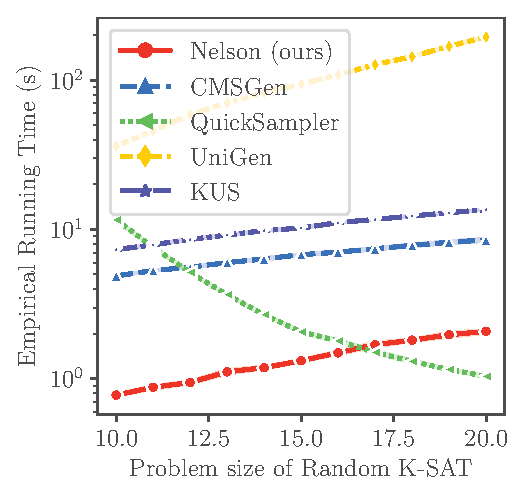
\includegraphics[width=0.49\linewidth]{exp/sampling.randkcnf.uniform.time.eps}
    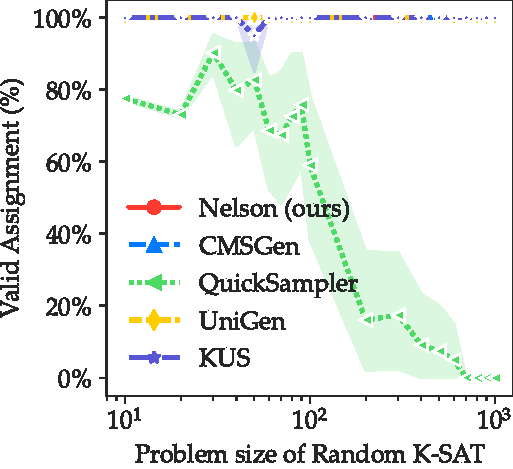
\includegraphics[width=0.50\linewidth]{exp/sampling.randkcnf.valid.pdf}
    \caption{Running time and the percentage of valid structures sampled uniformly at random from solutions of K-SAT problems. {Among all the problem sizes}, \nls always generates valid solutions and is the most efficient sampler.}
    \label{fig:uniform_sample}
\end{figure}

\begin{figure}[!t]
    \begin{minipage}{.53\linewidth}
        \centering
        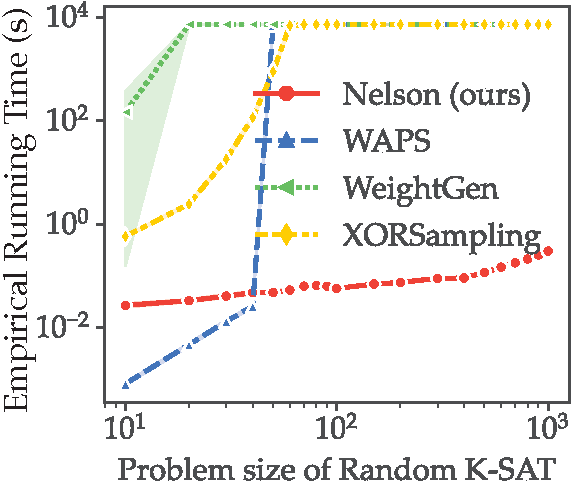
\includegraphics[width=1\linewidth]{exp/sampling.randkcnf.weighted-crop.pdf}
    \end{minipage}%
    \begin{minipage}{.47\linewidth}
        \raggedleft
        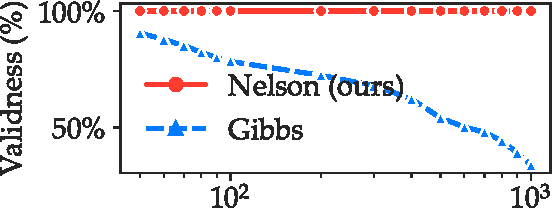
\includegraphics[width=0.99\linewidth]{exp/valid.randkcnf.weighted.pdf}\\
        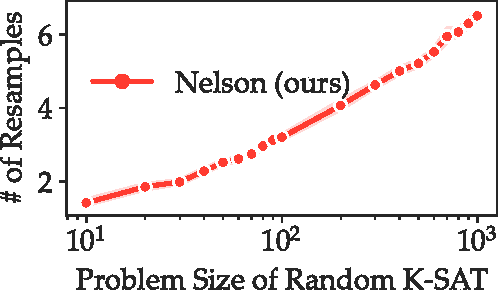
\includegraphics[width=0.89\linewidth]{exp/resample.randkcnf.weighted.pdf}
    \end{minipage}
    \caption{Running time, the percentage of valid solutions generated, and rounds of resampling for weighted sample generation of K-SAT solutions. {Among all the problem sizes}, \nls scales the best among all approaches and always generates valid solutions. }
    \label{fig:weighted_sample}
\end{figure}

\subsubsection*{Ablation Study} We also evaluated the samplers' efficiency in isolation (not embedded in
learning).
%
The sampling cases we considered are uniform and weighted (mainly following the
experiment setting in~\citep{DBLP:conf/aaai/ChakrabortyM19}).
%
In weighted sampling, the weights are specified by fixed values to the single
factors in Eq.~\eqref{eq:constr_mrf_single}.
%
In the uniform sampling case in Fig.~\ref{fig:uniform_sample}, \nls and
Quicksampler require much less time to draw samples compared to other
approaches. However, the solutions generated by Quicksampler rarely satisfy
constraints. In the weighted sampling case in Fig.~\ref{fig:weighted_sample},
\nls scales better than all the competing samplers as the sizes of the $K$-SAT
problems increase.

\begin{table}[!t]
    \centering
    \caption{Sample efficiency and learning performance of the sink-free orientation task. \nls is the most efficient (see Training Time Per Epoch) and always generates valid assignments (see Validness), has the smallest error approximating gradients, and has the best learning performance (see MAP@10) among all baselines.}\label{tab:sink-free}
    \begin{tabular}{r|rrr}
        \hline
        Problem & \multicolumn{3}{c}{{(a) Training Time Per Epoch} (Mins) ($\downarrow$)}                                                             \\ \cline{2-4}
        size    & \nls                                                                                                 & Gibbs    & CMSGen            \\
        \hline
        $10$    & $\mathbf{0.53}$                                                                                      & $9.85$   & $0.69$            \\
        $20$    & $\mathbf{0.53}$                                                                                      & $80.12$  & $1.93$            \\
        $30$    & $\mathbf{0.72}$                                                                                      & $256.38$ & $3.65$            \\
        $40$    & $\mathbf{0.93}$                                                                                      & $777.01$ & $5.99$            \\
        $50$    & $\mathbf{1.17}$                                                                                      & T.O.     & $9.08$            \\
        %
        %
        %
        %
        %
        \hline
                & \multicolumn{3}{c}{{(b) Validness of Orientations} ($\%$) ($\uparrow$)}                                                             \\ \hline
        $7$     & $\mathbf{100}$                                                                                       & $50.16$  & $\mathbf{100}$    \\   %
        $8$     & $\mathbf{100}$                                                                                       & $64.63$  & $\mathbf{100}$    \\ %
        $9$     & $\mathbf{100}$                                                                                       & $47.20$  & $\mathbf{100}$    \\  %
        $10$    & $\mathbf{100}$                                                                                       & $62.60$  & $\mathbf{100}$    \\ %
        $11$    & $\mathbf{100}$                                                                                       & $84.95$  & $\mathbf{100}$    \\ %
        %
        %
        %
        %
        \hline
                & \multicolumn{3}{c}{(c) Approximation Error of  $\nabla\log Z_{\mathcal{C}}(\theta)$  ($\downarrow$)}                                \\ \hline
        $5$     & $\mathbf{0.01}$                                                                                      & $0.09$   & $0.21$            \\
        %
        $7$     & $\mathbf{0.05}$                                                                                      & $0.08$   & $2.37$            \\
        $9$     & $\mathbf{0.03}$                                                                                      & $0.11$   & $2.37$            \\
        $11$    & $\mathbf{0.04}$                                                                                      & $0.17$   & $8.62$            \\
        $13$    & $\mathbf{0.05}$                                                                                      & $0.28$   & $11.27$           \\
        \hline
                & \multicolumn{3}{c}{(d) MAP@10 (\%) ($\uparrow$) }                                                                                   \\ \hline
        $10$    & $61.14$                                                                                              & $60.01$  & $\mathbf{64.56}$  \\
        $20$    & $\mathbf{55.26}$                                                                                     & $55.20$  & $47.79$           \\
        $30$    & $\mathbf{100.00}$                                                                                    & $96.29$  & $\mathbf{100.00}$ \\
        $40$    & $\mathbf{40.01}$                                                                                     & $39.88$  & $38.90$           \\
        $50$    & $\mathbf{46.12}$                                                                                     & T.O.     & $42.11$           \\
        \hline
    \end{tabular}
\end{table}

\subsection{Sink-Free Orientation in Undirected Graphs}
\noindent\textbf{Task Definition \& Dataset}  A \textit{sink-free} orientation of an undirected graph is a choice of orientation for each arc such that every vertex has at least one outgoing arc~\citep{DBLP:journals/combinatorics/CohnPP02}. This task has wide applications in robotics routing and IoT network configuration~\citep{takahashi2009communication}. Even though finding a sink-free orientation is tractable, sampling a sink-free orientation from the space of all orientations is still \#P-hard. Given a training set of preferred orientations $\mathcal{D}$ for the graph, the \textit{learning} task is to maximize the log-likelihood of the orientations seen in the training set. The \textit{inference} task is to generate valid orientations that resemble those in the training set. To generate the training set, we use the Erd\H{o}s-R\'enyi random graph  from the NetworkX library. The problem size is characterized by the number of vertices in the graph. The baselines we consider are CD-based learning with Gibbs sampling and CMSGen.

\subsubsection*{Learning Quality} In Table~\ref{tab:sink-free}(a), we show the proposed \nls method takes much
less time to train MRF for one epoch than the competing approaches.
Furthermore, in Table~\ref{tab:sink-free}(b), \nls and CMSGen generate $100\%$
valid orientations of the graph while the Gibbs-based model does not.
%
Note the constraints for this task satisfy Condition~\ref{cond:extreme}, hence
\nls sampler's performance is guaranteed by Theorem~\ref{th:product-dist}.
%
In Table~\ref{tab:sink-free}(c), \nls attains the smallest approximation error
for the gradient (in Eq.~\ref{eq:gradient}) compared to baselines. Finally,
\nls learns a higher MAP@10 than CMSGen. The Gibbs-based approach times out for
problem sizes larger than $40$. In summary, our \nls is the best-performing
algorithm for this task.

\subsection{Learn Vehicle Delivery Routes}
\subsubsection*{Task Definition \&  Dataset} Given a set of locations to visit, the task is to generate a sequence to visit
these locations in which each location is visited once and only once and the
sequence closely resembles the trend presented in the training data. The
training data are such routes collected in the past. The dataset is constructed
from TSPLIB, which consists of $29$ cities in Bavaria, Germany. The constraints
for this problem do not satisfy Condition~\ref{cond:extreme}. We still apply
the proposed method to evaluate if the \nls algorithm can handle those general
hard constraints.

In Fig.~\ref{fig:route}, we see \nls can obtain samples of this delivery
problem efficiently. We measure the number of resamples taken as well as the
corresponding time used by the \nls method. \nls takes roughly 50
resamples with an average time of $0.3$ seconds to draw a batch (the batch size
is $100$) of valid visiting sequences.

\begin{figure}[!t]
    \centering
    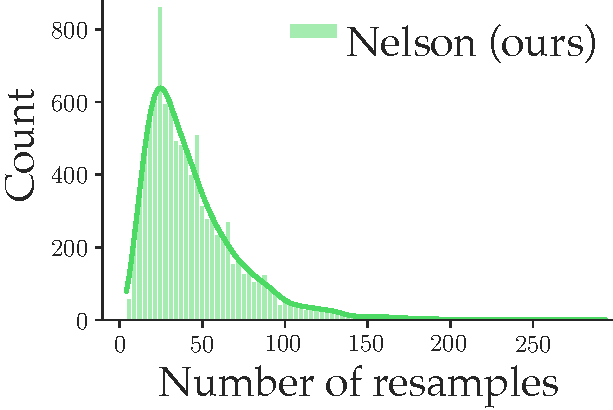
\includegraphics[width=0.495\linewidth]{exp/vehicle.resamples.pdf}
    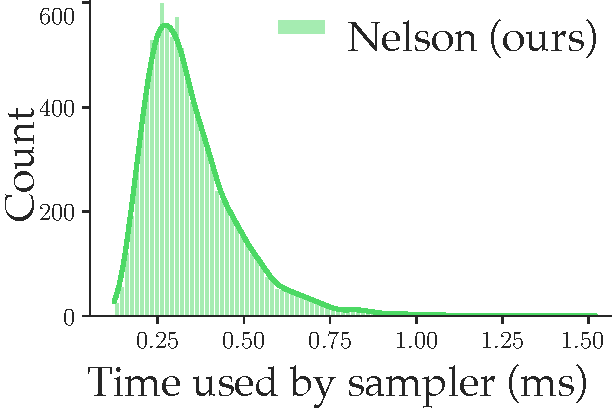
\includegraphics[width=0.495\linewidth]{exp/vehicle.time.pdf}
    \caption{Frequency histograms for the number of resamples and the total time of the \nls method for uniformly sampling visiting paths for the vehicle routing problem.}
    \label{fig:route}
\end{figure}
\section{Chapter Recap}
Before we move on to the more technical part, let us recap the research problems
this chapter wants to address. In this chapter, we present \nls, which embeds a
sampler based on \lovasz Local Lemma into the contrastive divergence learning
of Markov random fields. The embedding is fully differentiable. This approach
allows us to learn generative models over constrained domains, which presents
significant challenges to other state-of-the-art models. We also give sound
proofs of the performance of the LLL-based sampler.
%
Experimental results on several real-world domains reveal that \nls learns to
generate 100\% valid structures, while baselines either time out or cannot
generate valid structures.
%
\nls also outperforms other approaches in the running times and in various learning metrics. %

\section{Probability Distribution  of Algorithm~\ref{alg:lll-sampler}}\label{appendix:prob-dist}
%

\subsection{Definitions and Notations}
This section is for the proofs related to the probability distribution in the
proposed Algorithm~\ref{alg:lll-sampler}. For convenience, commonly used
notations are listed in Table~\ref{tab:quantifier}. We make some slight changes
to some notations that appear in this chapter to make sure they are consistent
and well-defined in this proof.

Similar to the previous
analysis~\citep{DBLP:journals/jacm/GuoJL19,DBLP:journals/arxiv/jerrum2021}, we
begin by introducing the concept ``dependency graph'' (in
Definition~\ref{def:dep-graph}) for the constraints $\mathcal{C}$.

\begin{definition}[Dependency Graph] \label{def:dep-graph}
    The dependency graph is $G=(\mathcal{C},E)$, where the vertex set is the set of constraints $\mathcal{C}$.  Two vertices $c_i$ and $c_j$ are connected with an edge $(c_i,c_j)\in E$ if and only if they are defined on at least one common random variable, i.e., $\var(c_i)\cap\var(c_j) \neq \emptyset$.
\end{definition}

For keeping track of the whole sampling procedure, we need the concept
``sampling record'' (in
Definition~\ref{def:record})~\citep{DBLP:journals/jacm/GuoJL19}, which lists the
broken constraints at every round in Algorithm~\ref{alg:lll-sampler}. It is
also known as the witness tree in~\citep{DBLP:journals/jacm/MoserT10}. This
allows us to check the constraint satisfaction of the assignment at every
round.

Under Condition~\ref{cond:extreme}, for any edge in the dependency graph
$(c_i,c_j) \in E$, either $\mathbf{1}(x,c_i)=1$ or $\mathbf{1}(x,c_j)=1$ for
all $x\in \mathcal{X}$. In other words, two constraints with shared related
variables, representing two \textit{adjacent vertices} in the dependency graph
$G$, are not broken simultaneously. Thus, the constraints in record $S_t$ form
an \textit{independent set}\footnote{A set of vertices with no two adjacent
    vertices in the graph.} over the dependency graph under
Condition~\ref{cond:extreme}.

\begin{definition}[Sampling Record] \label{def:record}
    Given dependency graph $G(\mathcal{C},E)$, let $X_t=x$ be  one possible assignment obtained at round $t$ of Algorithm~\ref{alg:lll-sampler}. Let $S_t\subseteq \mathcal{C}$ be the set of vertices in graph $G$ (subset of constraints) that $x$ violates
    \begin{align}
        S_t = \{c_i|c_i\in \mathcal{C}\text{ and } \mathbf{1}(x,c_i)=0\},
    \end{align}
    where indicator function $\mathbf{1}(x,c_i)=0$ implies  $x$ violates constraint $c_i$  at round $t$.
    Define the sampling record as the sequence of violated constraints  $S_1,\ldots,S_t$ throughout the execution.
\end{definition}

At round $t$ ($t \geq 1$) of Algorithm~\ref{alg:lll-sampler}, suppose the
set of violated constraints is $S_t\subseteq \mathcal{C}$. The constraints that are
not adjacent to $S_t$ in the dependency graph are still satisfied after
re-sampling. The only possible constraints that might be broken after the
re-sample operation are among $S_t$ itself, or those constraints directly
connected to $S_t$ in the dependency graph. Therefore,
\begin{equation*}
    S_{t+1} \subset \Gamma(S_t),    \qquad \text{ for all } t\ge 1.
\end{equation*}
where $\Gamma(S_t)$ is the set of vertices of $S_t$ and its adjacent neighbors
in the dependency graph $G$ (see Table~\ref{tab:quantifier}).  When Algorithm~\ref{alg:lll-sampler} terminates at round $T+1$, no  constraints are violated anymore, i.e., $S_{T+1}=\emptyset$.  To summarize the above discussion on a sampling record by Algorithm~\ref{alg:lll-sampler}, we have the following Claim~\ref{claim:record}.
\begin{claim}~\label{claim:record}
    Under Condition~\ref{cond:extreme}, a potential sampling record of length $T+1$ by the Algorithm~\ref{alg:lll-sampler} is a sequence of independent sets: $S_1, S_2, \ldots,S_T,\emptyset$ with
    \begin{enumerate}
        \item $S_{t+1} \subseteq \Gamma(S_{t})$ and $S_t\neq\emptyset$, for $1 \leq t\leq T$;
        \item $S_{T+1}=\emptyset$.
    \end{enumerate}
\end{claim}

\begin{table}[!t]
    \tiny
    \centering
    \caption{Summary of all the notations used in the theoretical analysis of Algorithm~\ref{alg:lll-sampler}.}\label{tab:quantifier}
    \begin{tabular}{ll}
        \hline
        Notation                                         & Definition                                                                                   \\
        \hline
        $X=\{X_i\}_{i=1}^n$                              & set of discrete random variables                                                             \\
        \hline
        $x\in\mathcal{X}$                                & possible assignments for variables $X$                                                       \\
        \hline
        $x_i\in\mathcal{X}_i$                            & variable $X_i$ can take all values in $\mathcal{X}_i$                                        \\
        \hline
        $\mathcal{C}=\{c_j\}_{j=1}^{m}$                  & given constraints                                                                            \\
        \hline
        $S_t\subseteq\mathcal{C}$                        & subset of constraints violated at round  $t$ of Algorithm~\ref{alg:lll-sampler}              \\
        \hline
        $G(\mathcal{C},E)$                               & the dependency graph (in Definition~\ref{def:dep-graph})                                     \\
        \hline
        $\var(c_j)$                                      & the indices of domain variables that are related to constraint $c_j$                         \\
        \hline
        $\var(S_t)$                                      & the indices for domain variables that are related to constraints $S_t$                       \\
        \hline
        $\Gamma(c_j)$                                    & $c_j$ and its direct neighbors in the dependency graph                                       \\
        \hline
        $\Gamma(S_t)$                                    & $S_t$ and direct neighbors of $S_t$ in the      dependency graph                             \\
        \hline
        $\mathcal{C}\backslash \Gamma(S_t)$              & all constraints in $\mathcal{C}$ but not in $\Gamma(S_t)$                                    \\
        \hline
        $S_1,\ldots,S_{T},\emptyset$                     & a sampling record of Algorithm~\ref{alg:lll-sampler}  (in Definition~\ref{def:record})       \\
        \hline
        $\mathbf{1}(x,c_i)$                              & indicator function that evaluates if    assignment $x$ satisfies constraint $c_i$            \\
        \hline
        $\mathbf{1}(x,S_t)$                              & indicator function that evaluates if assignment $x$ satisfies constraints in $S_t$           \\
        \hline
        $\mathbf{1}(x,\mathcal{C})$                      & indicator function that evaluates if  assignment $x$ satisfies all constraints $\mathcal{C}$ \\
        \hline
        $P_{\theta}(X|\mathcal{C}\backslash\Gamma(S_t))$ & see Definition~\ref{def:general-cmrf}                                                        \\
        \hline
        $\p(X|S_t)$                                      & see Definition~\ref{def:prs-prob}                                                            \\
        \hline
    \end{tabular}
\end{table}

\subsubsection*{Extra Notations related to Constrained MRF}
The constrained MRF model over constraint set $\mathcal{C}$ is defined as:
\begin{align*}
    P_{\theta}(X=x|\mathcal{C}) & =\frac{\exp(\sum_{i=1}^n\theta_i x_i)\mathbf{1}(x,\mathcal{C})}{\sum_{x'\in\mathcal{X}}\exp(\sum_{i=1}^n\theta_i x'_i)\mathbf{1}(x',\mathcal{C})}
\end{align*}
where the partition function only sums over valid assignments in $\mathcal{X}$. Note that $C(x)$ in Equation~\eqref{eq:constr_mrf_single} is the same as $\mathbf{1}(x,\mathcal{C})$ in the above equation. We slightly change the notations for consistency in this proof. Also notice that the output distribution can no longer be factorized after constraints are enforced, since the partition function cannot be factorized. Our task is to draw samples from this distribution.

To analyze the intermediate steps in Algorithm~\ref{alg:lll-sampler}, we
further need to define the following notations.
\begin{definition}  \label{def:general-cmrf}
    The constrained MRF distribution for constraints $\mathcal{C}\backslash \Gamma(S_t)$ is
    \begin{equation*}
        \begin{aligned}
            P_{\theta}(X=x|\mathcal{C}\backslash \Gamma(S_t)) & =\frac{\exp(\sum_{i=1}^n\theta_i x_i)\mathbf{1}(x,\mathcal{C}\backslash \Gamma(S_t))}{\sum_{x'\in\mathcal{X}}\exp(\sum_{i=1}^n\theta_i x'_i)\mathbf{1}(x',\mathcal{C}\backslash \Gamma(S_t))}
        \end{aligned}
    \end{equation*}
\end{definition}

\begin{definition}  \label{def:prs-prob}
    At round $t$ of Algorithm~\ref{alg:lll-sampler}, assume $S_t\subseteq\mathcal{C}$ is the set of broken constraints. Define $\p(X_{t+1}=x|S_1,\ldots, S_t)$ to be the probability of obtaining a new assignment $x$ after we re-sample random variables indexed by $\var(S_t)$.
\end{definition}
\subsection{Ratio Property Lemma}

\begin{lemma}[Ratio Property] \label{lem:ratio-prob}
    Under Condition~\ref{cond:extreme}, assume Algorithm~\ref{alg:lll-sampler} is at round $t$. Conditioning on observing one possible sampling record $S_1,\ldots,S_t$, Algorithm~\ref{alg:lll-sampler} step 4 will re-sample variables in $\var(S_t)$ at round $t+1$. Let $x,x'\in\mathcal{X}$ be two possible assignments after this re-sample.  The probability ratio  of obtaining these two results equals that under constrained MRF
    $P_{\theta}(x|\mathcal{C}\backslash \Gamma(S_t))$:
    \begin{equation} \label{eq:ratio}
        \frac{\p(X_{t+1}= x |S_1,\ldots, S_t)}{\p(X_{t+1}= x'|S_1,\ldots, S_t)} = \frac{P_{\theta}(X = x |\mathcal{C}\backslash \Gamma(S_t))}{P_{\theta}(X = x'|\mathcal{C}\backslash \Gamma(S_t))},
    \end{equation}
    where $\p(X_{t+1}= x |S_1,\ldots, S_t)$ is the probability that Algorithm~\ref{alg:lll-sampler} step 4 produces assignment $x$ at round $t+1$, conditioning on the observed record $S_1,\ldots, S_t$ and re-sampling $\var(S_t)$. $P_{\theta}(X = x |\mathcal{C}\backslash \Gamma(S_t))$ is the constrained MRF (for the constraints  $\mathcal{C}\backslash \Gamma(S_t)$) probability on assignment $x$.
    \begin{proof}
        During the intermediate step of the algorithm, assume the set of constraints $S_t$ is violated. We want to re-sample variables indexed by $\var(S_t)$, so  variables indexed by $\var(\mathcal{C}\backslash\Gamma(S_t))$ won't change assignments. Also, because $\Gamma(S_t)$ is the largest possible set of constraints that can be infected by the re-sample, constraints $\mathcal{C}\backslash \Gamma(S_t)$ are still satisfied after the re-sample.

        At round $t$, we re-sample variables in $\var(S_t)$ according to step 4 in
        Algorithm~\ref{alg:lll-sampler}, we thus have:
        \begin{equation*}
            \p(X^{t+1}_{\var(S_t)}=x_{\var(S_t)}|S_1 \ldots S_t)=\underset{{i\in\var(S_t)}}{\prod}\frac{\exp(\theta_i x_i)}{\underset{x'_i\in \mathcal{X}_i}{\sum}\exp(\theta_ix'_i)}.
        \end{equation*}
        Here the notation $X^{t+1}_{\var(S_t)}=x_{\var(S_t)}$ means $X_i=x_i$ for $i\in\var(S_t)$ at round $t$. For any two possible assignments $x,x'$ after the re-sample,
        \begin{equation*}
            x_i=x'_i,\quad \text{ for }i\in \{1,\ldots,n\}\backslash \var(S_t)
        \end{equation*}
        since the remaining variables' assignments are kept the same after re-sampling. Thus, we can have the ratio:
        \begin{equation}\label{eq:ratio-nelson}
            \frac{\p(X_{t+1}=x|S_1,\ldots,S_t)}{\p(X_{t+1}=x'|S_1,\ldots, S_t)}=\frac{\exp(\sum_{i\in\var(S_t)}\theta_ix_i)}{\exp(\sum_{i\in\var(S_t)}\theta_ix'_i)} =\frac{\exp(\sum_{i\in\var(\Gamma(S_t))}\theta_ix_i)}{\exp(\sum_{i\in\var(\Gamma(S_t))}\theta_ix'_i)}.
        \end{equation}
        For the last step, since every assignment outside $\var(S_t)$ is not changed, we can enlarge the index set of summation to $\Gamma(S_t)$ by multiplying
        \begin{align*}
            1 = \frac{\exp(\sum_{i\in\var(\Gamma(S_t)) \backslash \var(S_t)}\theta_ix_i)}{\exp(\sum_{i\in\var(\Gamma(S_t))\backslash \var(S_t)}\theta_ix'_i)}.
        \end{align*}
        After re-sampling, we know $x$ must satisfy the constraints $\mathcal{C}\backslash\Gamma(S_t)$. Thus, the probability of this $x$ conditioned on constraints $\mathcal{C}\backslash\Gamma(S_t)$ holding in the constrained MRF model is:
        \begin{align*}
              & P_{\theta}(X=x|\mathcal{C} \backslash \Gamma(S_t))
            =\frac{\exp(\sum_{i=1}^n\theta_i x_i)\mathbf{1}(x,\mathcal{C}\backslash \Gamma(S_t))}{\sum_{x'\in\mathcal{X}} \exp(\sum_{i=1}^n\theta_i x'_i)\mathbf{1}\left(x',\mathcal{C}\backslash \Gamma(S_t)\right)} \nonumber \\
            = & \frac{\exp(\sum_{i=1}^n\theta_i x_i)}{\sum_{x'\in\mathcal{X}} \exp(\sum_{i=1}^n\theta_i x'_i)\mathbf{1}\left(x',\mathcal{C}\backslash \Gamma(S_t)\right)}.
        \end{align*}
        In the constrained MRF model (for constraints  $\mathcal{C}\backslash\Gamma(S_t)$), the ratio of these two probabilistic assignments $x,x'$ is:
        \begin{equation}\label{eq:ratio-cmrf}
            \begin{aligned}
                \frac{P_{\theta}(X=x|\mathcal{C}\backslash \Gamma(S_t))}{P_{\theta}(X=x'|\mathcal{C}\backslash\Gamma(S_t))}=\frac{\exp(\sum_{i\in \var(\Gamma(S_t))}\theta_ix_i)}{\exp(\sum_{i\in \var(\Gamma(S_t))}\theta_ix'_i)},
            \end{aligned}
        \end{equation}
        because the $x_i$ outside $\var(\Gamma(S_t))$ remain the same. Note that $x,x'$ are two possible assignments produced according to step 4 in Algorithm~\ref{alg:lll-sampler} at round $t$.
        Combining Equation~\eqref{eq:ratio-nelson} and Equation~\eqref{eq:ratio-cmrf}, we conclude that:
        \begin{equation*}
            \begin{aligned}
                \frac{\p(X_{t+1}=x|S_1,\ldots,S_t)}{\p(X_{t+1}=x'|S_1,\ldots,S_t)}=\frac{P_{\theta}(X=x|\mathcal{C}\backslash \Gamma(S_t))}{P_{\theta}(X=x'|\mathcal{C}\backslash\Gamma(S_t))}.
            \end{aligned}
        \end{equation*}
        The proof is finished.
    \end{proof}
\end{lemma}
\subsection{Proof of Theorem~\ref{th:product-dist}}
Suppose the re-sampling process terminates at round $T+1$ and we obtain a valid sample $x$. Upon the termination of Algorithm~\ref{alg:lll-sampler}, all the constraints are satisfied. So we have: $S_{T+1}=\emptyset$. In other words, $\mathbf{1}(x,\mathcal{C})=1$.

Let $x,x'$ be two possible valid assignments produced at round $T+1$ by the
Algorithm~\ref{alg:lll-sampler}. Using the analysis in
Lemma~\ref{lem:ratio-prob}, we can still have:
\begin{equation*}
    \frac{\p(X_{T+1}=x|S_1,\ldots, S_T)}{\p(X_{T+1}=x'|S_1,\ldots, S_T)}=\frac{\exp(\sum_{i\in\var(S_T)}\theta_ix_i)}{\exp(\sum_{i\in\var(S_T)}\theta_ix'_i)}.
\end{equation*}
The probability of this $x$ in the constrained MRF model  (for constraints  $\mathcal{C}$) is:
\begin{equation*}
    P_{\theta}(X=x|\mathcal{C})=\frac{\exp(\sum_{i=1}^n\theta_i x_i)\mathbf{1}(x,\mathcal{C})}{\sum_{x'\in\mathcal{X}}  \exp(\sum_{i=1}^n\theta_i x'_i)\mathbf{1}\left(x',\mathcal{C}\right)}
    =\frac{\exp(\sum_{i=1}^n\theta_i x_i)}{\sum_{x'\in\mathcal{X}}  \exp(\sum_{i=1}^n\theta_i x'_i)\mathbf{1}\left(x',\mathcal{C}\right)}.
\end{equation*}
Then we conclude that:
\begin{equation*}
    \frac{\p(X_{T+1}=x|S_1,\ldots, S_T)}{\p(X_{T+1}=x'|S_1,\ldots, S_T)}=\frac{P_{\theta}(X=x|\mathcal{C})}{P_{\theta}(X=x'|\mathcal{C})}.
\end{equation*}
Note that this ratio property holds for all the possible sampling records $S_1,\ldots, S_T,\emptyset$.

\subsubsection*{Summation of All Possible Sampling Records} Define $\p(S_1,\ldots,S_T)$ to be the probability of observing record
$S_1,\ldots,S_T$ by Algorithm~\ref{alg:lll-sampler}. For any possible sampling
record $S_1,\ldots,S_{T}, \emptyset$, the ratio property still holds:
\begin{equation*}
    \frac{\p(X_{T+1}=x|S_1,\ldots S_T)\p(S_1,\ldots,S_T)}{\p(X_{T+1}=x'|S_1,\ldots,S_T)\p(S_1,\ldots,S_T)}=\frac{P_{\theta}(X=x|\mathcal{C})}{P_{\theta}(X=x'|\mathcal{C})}
\end{equation*}
where the term $\p(S_1,\ldots,S_T)$ on the left-hand side (LHS) is actually the same.
After we sum over all possible sampling records $S_1,\ldots,S_{T},\emptyset$, the ratio property still holds. Let $\p(X_{T+1}=x)$ be the probability of obtaining one valid assignment $x$ by the execution of Algorithm~\ref{alg:lll-sampler}.
\begin{equation} \label{eq:ratio-final}
    \frac{\p(X_{T+1}=x)}{\p(X_{T+1}=x')}=\frac{\sum_{S_1,\ldots,S_T}\p(X_{T+1}=x|S_1,\ldots,S_T)\p(S_1,\ldots,S_T)}{\sum_{S_1,\ldots,S_T}\p(X_{T+1}=x'|S_1,\ldots,S_T)\p(S_1,\ldots,S_T)}=\frac{P_{\theta}(X=x|\mathcal{C})}{P_{\theta}(X=x'|\mathcal{C})}
\end{equation}

\subsubsection*{Sample Space Analysis At Termination}
We need one more statement to show Theorem~\ref{th:product-dist} holds. Let
$\mathcal{X}_{\text{LLL}}$ be the set of all possible assignments $x$ that can
be generated by Algorithm~\ref{alg:lll-sampler}:
\begin{equation*}
    \mathcal{X}_{\text{LLL}}=\bigcup_{S_1\ldots S_T}\{x|\p(X_{T+1}=x|S_1\ldots S_T) \neq 0 \text{ and } \p(S_1\ldots S_T)\neq 0\}.
\end{equation*}
{where $ \p(S_1\ldots S_T)\neq 0$ means $S_1,\ldots,S_T$ is a possible record. $\p(X_{T+1}=x|S_1\ldots S_T) \neq 0$ means it is possible to obtain $x$ given the record $S_1,\ldots,S_T$.}

Let $\mathcal{X}_{\mathcal{C}}$ be the set of assignments $x$ that satisfy all
the constraints in the constrained MRF (for constraints $\mathcal{C}$):
\begin{equation*}
    \mathcal{X}_{\mathcal{C}}=\{x|P_{\theta}(X=x|\mathcal{C}) \neq 0, \text{ for all }x\in\mathcal{X}\}.
\end{equation*}

\begin{lemma}\label{lem:space}
    $\mathcal{X}_{\text{LLL}}\subseteq\mathcal{X}_{\mathcal{C}}$ and $\mathcal{X}_{\mathcal{C}}\subseteq\mathcal{X}_{\text{LLL}}$, thus $\mathcal{X}_{\text{LLL}}=\mathcal{X}_{\mathcal{C}}$.
    \begin{proof}
        When Algorithm~\ref{alg:lll-sampler} terminates, it only produces valid assignments; thus, we must have: $\mathcal{X}_{\text{LLL}}\subseteq\mathcal{X}_{\mathcal{C}}$. On the other hand,   there is always a non-zero probability that Algorithm~\ref{alg:lll-sampler} will generate every valid assignment $x\in\mathcal{X}_\mathcal{C}$, which implies that $\mathcal{X}_{\mathcal{C}}\subseteq\mathcal{X}_{\text{LLL}}$. Therefore we can conclude that $\mathcal{X}_{\text{LLL}}=\mathcal{X}_{\mathcal{C}}$.
    \end{proof}
\end{lemma}
Lemma~\ref{lem:space} shows that the two distributions have the same sample space when Algorithm~\ref{alg:lll-sampler} terminates. What's more, Equation~\eqref{eq:ratio-final} shows they have the same probability ratio for any possible valid assignments $x,x'$. This shows that the execution of the Algorithm~\ref{alg:lll-sampler} is a random draw from the constrained MRF distribution $P_{\theta}(X=x|\mathcal{C})$. The proof of Theorem~\ref{th:product-dist} is finished.
\subsection{Difference to the Original Proof}
The main difference in the above proof to the existing proof in~\citep[Lemma
    7]{DBLP:journals/jacm/GuoJL19} is that: We show Lemma~\ref{lem:ratio-prob} that
characterizes the proportional ratio of getting different assignments of
variables, which is more general than the descriptive proof for \citep[Lemma
    7]{DBLP:journals/jacm/GuoJL19}.
\subsection{A Running Example in View of a Markov Chain} \label{appendix:running-example}
{We dedicate this section to demonstrating the execution of Algorithm~\ref{alg:lll-sampler} with Example~\ref{example:matrix}. Algorithm~\ref{alg:lll-sampler} can be viewed as a Markov chain, so  we will show the probability of obtaining valid samples is unbiased by running thousands of steps of the Markov chain. }
The constraints are $\mathcal{C}=\{c_1=(X_1\vee X_2), c_2=(\neg X_1 \vee X_3)\}$. We use the assignment of all the variables as the states $s_1,\ldots, s_8$ in the rounds of Algorithm~\ref{alg:lll-sampler}.
\begin{equation}
    \begin{aligned}
        s_1 & =(X_0=0,X_1=0,X_2=0) \\
        s_2 & =(X_0=0,X_1=0,X_2=1) \\
        s_3 & =(X_0=0,X_1=1,X_2=0) \\
        s_4 & =(X_0=0,X_1=1,X_2=1) \\
        s_5 & =(X_0=1,X_1=0,X_2=0) \\
        s_6 & =(X_0=1,X_1=0,X_2=1) \\
        s_7 & =(X_0=1,X_1=1,X_2=0) \\
        s_8 & =(X_0=1,X_1=1,X_2=1) \\
    \end{aligned}
\end{equation}
Here $s_1,s_2,s_3,s_4$ correspond to \textit{valid} assignments of variables with respect to the constraints $\mathcal{C}$ and $s_5,s_6,s_7,s_8$ correspond to \textit{invalid} assignments of variables, that require resampling.

For simplicity, we consider the uniform setting where
$\theta_1=\theta_2=\theta_3=0$. The goal is to sample every valid assignment with
equal probability. Therefore, the probability for every variable is:
\begin{equation*}
    P(X_i)=\begin{cases}
        \frac{1}{2} & \text{ for variable } X_i\text{ taking value }1 \\
        \frac{1}{2} & \text{ for variable } X_i\text{ taking value }0 \\
    \end{cases}
\end{equation*}
for $i=1,2, 3$. Based on Algorithm~\ref{alg:lll-sampler}, we know the probability of transferring from $s_i$ to $s_j$ ($1\le i,j\le 8$). Thus we can construct the transition matrix between every state:
\begin{equation}
    T=\begin{bNiceMatrix}[
            %   first-row,code-for-first-row=\normalsize,
            %   first-col,code-for-first-col=\normalsize,
        ]
            & s_1         & s_2         & s_3         & s_4         & s_5         & s_6         & s_7         & s_8         \\
        s_1 & \mathbf{1}  & 0           & 0           & 0           & 0           & 0           & 0           & 0           \\
        s_2 & 0           & \mathbf{1}  & 0           & 0           & 0           & 0           & 0           & 0           \\
        s_3 & 0           & 0           & \mathbf{1}  & 0           & 0           & 0           & 0           & 0           \\
        s_4 & 0           & 0           & 0           & \mathbf{1}  & 0           & 0           & 0           & 0           \\
        s_5 & \frac{1}{4} & \frac{1}{4} & \frac{1}{4} & 0           & \frac{1}{4} & 0           & 0           & 0           \\
        s_6 & 0           & \frac{1}{4} & 0           & 0           & \frac{1}{4} & \frac{1}{4} & 0           & \frac{1}{4} \\
        s_7 & \frac{1}{4} & 0           & \frac{1}{4} & \frac{1}{4} & 0           & 0           & \frac{1}{4} & 0           \\
        s_8 & 0           & 0           & \frac{1}{4} & 0           & 0           & \frac{1}{4} & \frac{1}{4} & \frac{1}{4} \\
    \end{bNiceMatrix}
\end{equation}
where $T_{ij}=T(s_i,s_j)$ denotes the transition probability from state $s_i$ to state $s_j$.

    {Taking state $s_5$ as an example, it violates constraint $C_2$ thus $X_2,X_3$ will be resampled. There are 4 possible assignments of  $X_2,X_3$, which correspond to states $\{s_1,s_2,s_3,s_5\}$. Since each variable is resampled uniformly at random, the probability of transition from state $s_5$ to the states $\{s_1,s_2,s_3,s_5\}$ is $1/4$. The Algorithm~\ref{alg:lll-sampler} will terminate once it reaches states $\{s_1,s_2,s_3,s_4\}$, which corresponds to the (valid) state only transitioning to itself with probability 1. Thus we find $T(s_i,s_i)=1$ for $i=1,2,3,4$.}

For a randomly initialized assignment:
\begin{equation}
    x=\begin{bNiceMatrix}[
            %   first-row,code-for-first-row=\normalsize,
            %   first-col,code-for-first-col=\normalsize,
        ]
         & s_1         & s_2         & s_3         & s_4         & s_5         & s_6         & s_7         & s_8         \\
         & \frac{1}{8} & \frac{1}{8} & \frac{1}{8} & \frac{1}{8} & \frac{1}{8} & \frac{1}{8} & \frac{1}{8} & \frac{1}{8} \\
    \end{bNiceMatrix}
\end{equation}
that has an equal probability of being any state.
After executing Algorithm~\ref{alg:lll-sampler} for 2000 steps, we have:
\begin{equation}
    T^{2000}=\begin{bNiceMatrix}[
            %   first-row,code-for-first-row=\normalsize,
            %   first-col,code-for-first-col=\normalsize,
        ]
            & s_1         & s_2         & s_3         & s_4         & s_5 & s_6 & s_7 & s_8         \\
        s_1 & \mathbf{1}  & 0           & 0           & 0           & 0   & 0   & 0   & 0           \\
        s_2 & 0           & \mathbf{1}  & 0           & 0           & 0   & 0   & 0   & 0           \\
        s_3 & 0           & 0           & \mathbf{1}  & 0           & 0   & 0   & 0   & 0           \\
        s_4 & 0           & 0           & 0           & \mathbf{1}  & 0   & 0   & 0   & 0           \\
        s_5 & \frac{1}{3} & \frac{1}{3} & \frac{1}{3} & 0           & 0   & 0   & 0   & 0           \\
        s_6 & \frac{1}{6} & \frac{1}{2} & \frac{1}{6} & \frac{1}{6} & 0   & 0   & 0   & \frac{1}{4} \\
        s_7 & \frac{1}{3} & 0           & \frac{1}{3} & \frac{1}{3} & 0   & 0   & 0   & 0           \\
        s_8 & \frac{1}{6} & \frac{1}{6} & \frac{1}{6} & \frac{1}{2} & 0   & 0   & 0   & 0           \\
    \end{bNiceMatrix},
\end{equation}
\begin{equation}
    xT^{2000}=\begin{bNiceMatrix}[
            %   first-row,code-for-first-row=\normalsize,
            %   first-col,code-for-first-col=\normalsize,
        ]
         & s_1         & s_2         & s_3         & s_4         & s_5 & s_6 & s_7 & s_8 \\
         & \frac{1}{4} & \frac{1}{4} & \frac{1}{4} & \frac{1}{4} & 0   & 0   & 0   & 0   \\
    \end{bNiceMatrix}.
\end{equation}
This implies Algorithm~\ref{alg:lll-sampler} outputs every valid assignment with the same probability in the uniform setting, which follows the result in Theorem~\ref{th:product-dist}.
\section{Running Time Analysis of Algorithm~\ref{alg:lll-sampler}} \label{appendix:time-analysis}
We dedicate this section to showing the running time of Algorithm~\ref{alg:lll-sampler} on a general weighted case.
%
The expected running time of Algorithm~\ref{alg:lll-sampler} is determined by
the number of rounds of re-sampling.
%
Algorithm~\ref{alg:lll-sampler} re-samples all the related random variables
simultaneously in every single round.
%
However, it is hard to get an estimation of the exact total running time over
the \textit{random variables}. Instead, we can only have a loose upper bound of
the expected running time over the \textit{sequence of sampling records} (the
sequence of violated constraints).

The overall structure of the proof is similar to the proof in~\citep[Theorem
    13]{DBLP:journals/jacm/GuoJL19}. We show the difference in our proof at the end
of this section.

\subsection{Definitions and Notations}
We define the following terms to simplify our notations.
\begin{definition}  \label{def:p_q_st}
    Let $S_t$ be a subset of vertices in a dependency graph.
    1) Define $p_{S_t}$ as the probability of  constraints in $S_t$ being violated:
    \begin{equation} \label{eq:def-pst}
        p_{S_t}=\p\left(\bigwedge_{c_i \in S_t}\neg{c}_i \right)
    \end{equation}
    {where we use $\neg{c}_i $ to indicate the constraint $c_i$ is violated.}
    2) Define $q_{S_t}$ as the probability that only the constraints in $S_t$ are violated and nothing else.
    \begin{equation} \label{eq:definition-qst}
        q_{S_t}=\p\left(\bigwedge_{c_i \in S_t}\neg{c}_i \wedge \bigwedge_{c_j \in \mathcal{C}\backslash S_t}c_j\right)
    \end{equation}
    {where $\bigwedge_{c_i \in S_t}\neg{c}_i $ corresponds to only the constraints in $S_t$ being violated and $\bigwedge_{c_j \in \mathcal{C}\backslash S_t}c_j$ corresponds to all the rest of the constraints being satisfied.}
    So $q_{\{c_i\}}$ is the probability that only constraint $c_i$ is broken and all the rest still  hold. Similarly, $q_{\emptyset}$ denotes the probability that all the constraints are satisfied.
\end{definition}

\begin{lemma} \label{lem:recursion_start}
    Given Definition~\ref{def:p_q_st}, we can further expand $q_{S_t}$ under Condition~\ref{cond:extreme}:
    \begin{equation*}
        q_{S_t}= p_{S_t}\p \left( \wedge_{c_j \in \mathcal{C}\backslash \Gamma(S_t)}c_j\right)
    \end{equation*}
    \begin{proof}
        We can split $q_{S_t}$ into the probability of two independent events:
        \begin{align*}
            q_{S_t} & =\p\left(\bigwedge_{c_i \in S_t}\neg{c}_i \wedge \bigwedge_{c_j \in \mathcal{C}\backslash S_t}c_j\right)                   & \text{ By definition of $q_{S_t}$ in Equation~\eqref{eq:definition-qst}} \\
                    & =\p\left(\bigwedge_{c_i \in S_t}\neg{c}_i \wedge \bigwedge_{c_j \in \mathcal{C}\backslash \Gamma(S_t)}c_j\right)                                                                                      \\
                    & =\p\left(\bigwedge_{c_i \in S_t}\neg{c}_i\right) \p \left( \bigwedge_{c_j \in \mathcal{C}\backslash \Gamma(S_t)}c_j\right)                                                                            \\
                    & = p_{S_t}\p \left( \wedge_{c_j \in \mathcal{C}\backslash \Gamma(S_t)}c_j\right).                                           & \text{ By definition of $p_{S_t}$ in Equation~\eqref{eq:def-pst}}
        \end{align*}
        The second equality holds because under  Condition~\ref{cond:extreme}, adjacent vertices have zero probability. In other words, when we observe that constraints in $S_t$ are violated, constraints in $\Gamma(S_t)\backslash S_t$ cannot be violated. The third equality holds because the random variables in $\var(S_t)$ are \textit{independent of}
        those variables in $\var(\mathcal{C}\backslash\Gamma(S_t))$. {So we can apply $P(AB)=P(A)P(B)$ when the events $A,B$  are independent of each other.}
    \end{proof}
\end{lemma}

\begin{remark}[Equivalence of Record] \label{rem:equal}
    At round $t$ of Algorithm~\ref{alg:lll-sampler},  it finds all the constraints $S_t$ that are broken ($\bigwedge_{c_i \in S_t}\neg{c}_i $), which implies the rest of the constraints $\mathcal{C}\backslash \Gamma(S_t)$ are satisfied ($\bigwedge_{c_j \in \mathcal{C}\backslash S_t}c_j$). Thus the probability of observing $S_t$ in the record is equivalent to the following:
    \begin{align} \label{eq:st-expand}
        \p(S_t)=\p\left(\bigwedge_{c_i \in S_t}\neg{c}_i \wedge \bigwedge_{c_j \in \mathcal{C}\backslash S_t}c_j\right)
    \end{align}
\end{remark}

\begin{lemma} \label{eq:pair-prob}
    Given a possible sampling record $S_1$ $\ldots$ $S_{t-1}$,$S_t$ by Algorithm~\ref{alg:lll-sampler}, the following equality holds for the pair $(S_{t-1},S_t)$:
    \begin{equation*}
        \sum_{S_t}q_{S_t}=\p(\wedge_{c_i \in \mathcal{C}\backslash \Gamma(S_{t-1})}c_i)
    \end{equation*}
    \begin{proof}
        By Definition~\ref{def:record} of the sampling record, we have $S_t \subset \Gamma(S_{t-1})$. The  relationship of its complement would be:
        \begin{equation*}
            \mathcal{C}\backslash\Gamma(S_{t-1})\subset \mathcal{C}\backslash S_t.
        \end{equation*}
        Using the above result, we have:
        \begin{equation}\label{eq:subset}
            \p\left(\bigwedge_{c_j \in \mathcal{C}\backslash S_t}c_j \wedge \bigwedge_{c_k \in \mathcal{C}\backslash \Gamma(S_{t-1})}c_k \right)=
            \p\left(\bigwedge_{c_j \in \mathcal{C}\backslash S_t}c_j \right)
        \end{equation}

        Based on Remark~\ref{rem:equal} and Bayes's theorem, we have:
        \begin{equation} \label{eq:bayes}
            \begin{aligned}
                  & \p(S_t |\wedge_{c_i \in \mathcal{C}\backslash \Gamma(S_{t-1})}c_i) \nonumber                                                                                                                                                                                                                                                               \\
                = & \p\left(\bigwedge_{c_i \in S_t}\neg{c}_i \wedge \bigwedge_{c_j \in \mathcal{C}\backslash S_t}c_j \Big| \wedge_{c_k \in \mathcal{C}\backslash \Gamma(S_{t-1})}c_k \right)                                                                                        & \text{ By Equation~\eqref{eq:st-expand}}                                 \\
                = & \frac{\p\left(\bigwedge_{c_i \in S_t}\neg{c}_i \wedge \bigwedge_{c_j \in \mathcal{C}\backslash S_t}c_j \wedge \bigwedge_{c_k \in \mathcal{C}\backslash \Gamma(S_{t-1})}c_k \right)}{\p \left(\wedge_{c_i \in \mathcal{C}\backslash \Gamma(S_{t-1})}c_i\right) } & \text{By Bayes's formula}                                                \\
                = & \frac{\p\left(\bigwedge_{c_i \in S_t}\neg{c}_i \wedge \bigwedge_{c_k \in \mathcal{C}\backslash S_{t}}c_k \right)}{\p \left(\wedge_{c_i \in \mathcal{C}\backslash \Gamma(S_{t-1})}c_i\right) }                                                                   & \text{ By Equation~\eqref{eq:subset}}                                    \\
                = & \frac{q_{S_t} }{\p \left(\wedge_{c_i \in \mathcal{C}\backslash \Gamma(S_{t-1})}c_i\right) }.                                                                                                                                                                    & \text{ By definition of $q_{S_t}$ in Equation~\eqref{eq:definition-qst}}
            \end{aligned}
        \end{equation}

        The LHS of Equation~\eqref{eq:bayes} sums to one over $S_t$:
        $\sum_{S_t}\p(S_t |\wedge_{c_i \in \mathcal{C}\backslash
                \Gamma(S_{t-1})}c_i)=1$. Thus, summing over $S_t$ for the RHS of
        Equation~\eqref{eq:bayes}, we have:
        \begin{equation} \label{eq:summation-st}
            \begin{aligned}
                1=\sum_{S_t}\frac{q_{S_t} }{\p \left(\wedge_{c_i \in \mathcal{C}\backslash \Gamma(S_{t-1})}c_i\right) }=\frac{\sum_{S_t}q_{S_t} }{\p \left(\wedge_{c_i \in \mathcal{C}\backslash \Gamma(S_{t-1})}c_i\right) }
            \end{aligned}
        \end{equation}
        In the second equality, the reason that we can move the summation operator to  the numerator is that the denominator is a constant \textit{w.r.t.} all possible $S_t$. To be specific, given $S_t\subseteq\Gamma(S_{t-1})$, we have  $S_t$ is independent of $\mathcal{C}\backslash \Gamma(S_{t-1})$.
        Based on Equation~\eqref{eq:summation-st}, we finally obtain:
        \begin{equation*}
            \sum_{S_t}q_{S_t}=\p(\wedge_{c_i \in \mathcal{C}\backslash \Gamma(S_{t-1})}c_i).
        \end{equation*}
        The proof  is finished.
    \end{proof}
\end{lemma}

\begin{lemma} \label{lem:sample-record}
    The probability of observing the sampling record  $S_1,\ldots,S_T$ by Algorithm~\ref{alg:lll-sampler} under Condition~\ref{cond:extreme} is:
    \begin{equation}\label{pS_final}
        \p(S_1,\ldots ,S_T)=q_{S_T} \prod_{t=1}^{T-1} p_{S_t}
    \end{equation}
    \begin{proof}
        Given sampling record  $S_1,\ldots,S_{t-1}$, the conditional probability of observing the next record {$S_t,S'_t$} can be expanded  based on Lemma~\ref{lem:ratio-prob},
        \begin{equation*}
            \frac{\p(S_t | S_1, \ldots, S_{t-1})}{\p(S'_t | S_1, \ldots, S_{t-1})}=\frac{\p(S_t |\wedge_{c_i \in \mathcal{C}\backslash \Gamma(S_{t-1})}c_i)}{\p(S'_t |\wedge_{c_i \in \mathcal{C}\backslash \Gamma(S_{t-1})}c_i)}
        \end{equation*}
        Based on Equation~\eqref{eq:bayes}, we {can simplify the RHS of the above ratio equality and} obtain:
        \begin{equation*}
            \frac{\p(S_t | S_1, \ldots, S_{t-1})}{\p(S'_t | S_1, \ldots, S_{t-1})}=\frac{q_{S_t}}{q_{S'_t}}
        \end{equation*}
        Because of $\sum_{S_t}\p(S_t | S_1, \ldots, S_{t-1})=1$ and Equation~\eqref{eq:summation-st}, we can get:
        \begin{equation}\label{recursion_base}
            \p(S_t | S_1, \ldots, S_{t-1})=  \frac{q_{S_t}}{\p(\wedge_{c_i \in \mathcal{C}\backslash \Gamma(S_{t-1})}c_i)}
        \end{equation}
        We finally compute the probability of observing the sampling record $S_1\,\ldots, S_T$ by:
        \begin{equation*}
            \begin{aligned}
                \p(S_1\,\ldots ,S_T)= & \p(S_1)\prod_{t=2}^T\p(S_t | S_1,\ldots,S_{t-1})                                                        & \text{ By Chain rule}                                    \\
                =                     & q_{S_1}\prod_{t=2}^T \frac{q_{S_t}}{\p(\wedge_{c_i \in \mathcal{C}\backslash \Gamma(S_{t-1})}c_i)}      & \text{ By Equation~\eqref{recursion_base}}               \\
                =                     & q_{S_T} \prod_{t=2}^T \frac{q_{S_{t-1}}}{\p(\wedge_{c_i \in \mathcal{C}\backslash \Gamma(S_{t-1})}c_i)} & \text{ Left shift the numerator from $S_t$ to $S_{t-1}$} \\
                =                     & q_{S_T} \prod_{t=1}^{T-1} p_{S_t}                                                                       & \text{Plug in  Lemma~\ref{lem:recursion_start}}
            \end{aligned}
        \end{equation*}
        The proof is finished.
    \end{proof}
\end{lemma}

\subsection{An Upper Bound on Expected Running Time}
Suppose the expected number of samplings of constraint $c_i$ is $\e(T_i)$,
then the total running time will be:
\begin{equation*}
    \e(T) \le \sum_{i=1}^n \e (T_i)
\end{equation*}

Since each random variable has equal status, then the question comes down to
the computation of individual $T_i$'s expectation. Let $S_1,\ldots,S_T$ be any
record of the algorithm that successfully terminates, and $T_i(S_1,\ldots,S_T)$
be the total number of samplings related to constraint $c_i$ throughout this
record. Based on Lemma~\ref{lem:sample-record}, we have:
\begin{align*} \label{ti_formula}
    \e(T_i) & = \sum_{S_1,\ldots,S_T} \p(S_1,\ldots,S_T)T_i(S_1,\ldots,S_T)
\end{align*}
{So far, we have shown the original proof of our work. We leave the difference between our proof and the existing one in section \ref{apx:difference}.}

The rest of the computation can be done in the same way as the proof in
\citep{DBLP:journals/jacm/GuoJL19}. Thus we cite the necessary intermediate
steps in the existing work and finish the proof logic for the coherence of the
whole running time analysis.
\begin{lemma*}[\citep{DBLP:journals/jacm/GuoJL19} Lemma 12] \label{thm:runtime} Let $q_{\emptyset}$ be a non-zero probability that all the constraints are satisfied. Let $q_{\{c_j\}}$ denote the probability that only constraint $c_j$ is broken and the rest all hold. If $q_\emptyset>0$, then
    $\e(T_j) ={q_{\{c_j\}}}/{q_\emptyset}$.
\end{lemma*}

After incorporating our fix, we can conclude the upper bound on the expected
running time in Theorem~\ref{thm:time}.
\begin{theorem}[\citep{DBLP:journals/jacm/GuoJL19} Theorem 13] \label{thm:time} Under Condition~\ref{cond:extreme},
    the expected total number of re-samplings throughout the algorithm is then $\frac{1}{q_{\emptyset}}\sum_{j=1}^L q_{\{c_j\}}$.
\end{theorem}

\subsection{Difference to the Existing Proof}  \label{apx:difference}
The main difference in the above proof to the existing proof in~\citep[Theorem
    13]{DBLP:journals/jacm/GuoJL19} is that: based on
Equation~\eqref{recursion_base} and~\eqref{eq:bayes}, we show
\begin{equation*}
    \p(S_t | S_1, \ldots, S_{t-1})=\p(S_t |\wedge_{c_i \in \mathcal{C}\backslash \Gamma(S_{t-1})}c_i)
\end{equation*}
In \citep{DBLP:journals/jacm/GuoJL19}'s Equation~(9), the first step cannot hold without the above equality. The original paper uses this result directly without providing enough justification.
\section{Constrained MRF Model}\label{appendix:constrain-mrf}

\subsection{Single Variable Form of Constrained MRF}  \label{appendix:svf}
Here we provide an example of transforming MRF with pairwise and single
potential functions into a single potential form by introducing extra
variables. Given random variables $X_1,X_2,X_3$, we have the following example
MRF model:
\begin{align*}
    \phi_{\theta}(x_1,x_2,x_3) & =\theta_1 x_1+\theta_2 x_2+\theta_3 x_1 x_2           \\
    P_{\theta}(x)              & =\frac{\exp(\phi_{\theta}(x_1,x_2,x_3))}{Z({\theta})}
\end{align*}

In the above formula, we have a cross term $x_1 x_2$. Two Boolean variables can
have 4 different assignments in total. Therefore we can construct 4 extra
Boolean variables to encode all these assignments. To illustrate, we introduce
extra random variables $\hat{X}_{00}$, $\hat{X}_{01}$, $\hat{X}_{10}$,
$\hat{X}_{11}$. We further introduce extra constraints: When $X_1=0,X_2=0$, the
extra variables must take values: $\hat{X}_{00}=1$, $\hat{X}_{01}=0$,
$\hat{X}_{10}=0$, $\hat{X}_{11}=0$. See the rest of the constraints in
Table~\ref{tab:pairwise-to-single}.

\begin{table}
    \centering
    \begin{tabular}{cc|cccc}
        \hline
        $X_1$ & $X_2$ & $\hat{X}_{00}$, $\hat{X}_{01}$, $\hat{X}_{10}$, $\hat{X}_{11}$ \\ \hline
        $0$   & $0$   & $1, 0, 0, 0$                                                   \\
        $0$   & $1$   & $0, 1, 0, 0$                                                   \\
        $1$   & $0$   & $0, 0, 1, 0$                                                   \\
        $1$   & $1$   & $0, 0, 0, 1$                                                   \\
        \hline
    \end{tabular}
    \caption{4 constraints for converting pairwise terms in the potential function into single variable form.}
    \label{tab:pairwise-to-single}
\end{table}
Then the new potential function, including extended variables and pairwise to single variable constraints $\mathcal{C}$, is reformulated as:
\begin{align*}
    \hat{\phi}_{\theta}(x_1,x_2,x_3,\hat{x}_{00},\hat{x}_{01},\hat{x}_{10},\hat{x}_{11}) & =\theta_1 x_1+\theta_2 x_2+\theta_3 \hat{x}_{00}+ \theta_3 \hat{x}_{01}+\theta_3 \hat{x}_{10}+\theta_3 \hat{x}_{11}         \\
    P_{\theta}(x|\mathcal{C})                                                            & =\frac{\exp(\hat{\phi}_{\theta}(x_1,x_2,x_3,\hat{x}_{00},\hat{x}_{01},\hat{x}_{10},\hat{x}_{11}))}{Z_{\mathcal{C}}(\theta)}
\end{align*}
For clarity, the newly added constraints do not impact Condition~\ref{cond:extreme}. Since the single variable transformation in the MRFs model originates from~\citep{Sang2005}, it is not considered as our contribution.

\subsection{Gradient of $\log$-Partition Function $\nabla\log Z_\mathcal{C}(\theta)$}\label{appendix:partition}
We use the Chain rule of the gradient to give a detailed deduction of Equation~\eqref{eq:gradient}.
\begin{equation}\label{eq:full-gradient}
    \begin{aligned}
          & \nabla\log Z_\mathcal{C}(\theta)=\frac{\nabla Z_\mathcal{C}(\theta)}{Z_\mathcal{C}(\theta)}=\frac{1}{Z_\mathcal{C}(\theta)}\nabla\sum_{x\in \mathcal{X}}\exp\left( \phi_{\theta}(x)\right)C(x) \nonumber                                                                     \\
        = & \sum_{x\in\mathcal{X}} \frac{\exp(\phi_{\theta}(x))C(x) }{Z_\mathcal{C}(\theta)}{\nabla\phi_\theta(x)} =\sum_{x\in \mathcal{X}} P_\theta(x|\mathcal{C}) \nabla\phi_{\theta}(x) = \mathbb{E}_{x\sim P_{\theta}(\cdot|\mathcal{C})} \left({\nabla\phi_{\theta}(x)}\right).
    \end{aligned}
\end{equation}
{The above result shows the gradient of the constrained log-partition function is equivalent to the expectation of the gradient of the potential function $\nabla\phi_{\theta}$ over the model's distribution (\textit{i.e.}, $P_{\theta}(\tilde{x}|\mathcal{C})$). Therefore, we transform the gradient estimation problem into the problem of sampling from the current MRF model.}

\section{Experiment Settings and Configurations}
\label{appendix:exp-set}
\subsection{Implementation Details} \label{appendix:implementation}

\subsubsection*{Implementation of \nls} The proposed sampler can be implemented with NumPy, PyTorch, or JAX. We further
offer a ``batch version'' implementation, that draws a batch of samples in
parallel on GPU. The batched sampler is useful for those tasks that require a
huge number of samples to estimate the gradient with a small approximation
error.

    {In Section~\ref{sec:nls}, we define  vector of assignment  $x^t=(x^t_1, \dots, x^t_n)$,
        where $x_i^t$ is the assignment of variable $X_i$ in the $t$-th round of Algorithm~\ref{alg:lll-sampler}. $x^t_i=1$ denotes  variable $X_i$ takes value $1$ (or true). In the batch version, we define the matrix for a batch  of assignments. Let $b$ be the batch size. We have}
\begin{equation*}
    x^{t}=\begin{bmatrix}
        x^t_{11} & \dots  & x^t_{1n} \\
        \vdots   & \ddots & \vdots   \\
        x^t_{b1} & \dots  & x^t_{bn} \\
    \end{bmatrix}
\end{equation*}
{In the following part, we provide the detailed computation pipeline for the batch version of the proposed algorithm.}

\subsubsection*{Initialization} {The first step is to sample an initial assignment of $X$ from the given marginal probability vector $P$:}
\begin{equation}
    x^1_{li} = \begin{cases}
        1 & \text{if } u_{li}> P_i, \\
        0 & \text{otherwise}.       \\
    \end{cases},\quad \text{ if} 1\le i\le n, 1\le l\le b
\end{equation}
{Here $u_{li}$ is sampled from the uniform distribution over $[0,1]$.}

\subsubsection*{Check Constraint Satisfaction} { The second step extracts which constraint is violated. Given an assignment $x^t$ at round $t\ge 1$, tensor $W$ and matrix $b$, the computation of tensor $Z^t$ is:}
\begin{equation*}
    Z^t_{ljk} =\sum_{i=1}^n W_{jki} x_{li}^t+b_{jk},
\end{equation*}
{The special  multiplication between tensor and matrix can be efficiently implemented with the  Einstein summation\footnote{\url{https://github.com/dgasmith/opt_einsum}}.
%
Note that $Z^t_{ljk}=1$ indicates for $l$-th batched assignment $x_l$, the
$k$-th literal of $j$-th clause is true (takes value $1$). Next, we compute
$S^t_{lj}$ as:}
\begin{align*}
    S^t_{lj} & =1-\max_{1\le k\le K} Z^t_{ljk}, \quad \text{ for } 1\le j\le L, 1\le l\le b
\end{align*}
{Here $S^t_{lj}=1$ indicates $x_l^t$ violates $j$-th clause.
%
We can check $\sum_{l=1}^b\sum_{j=1}^LS^t_{lj}\neq 0$ to see if any clause is
violated for the current batch of assignments, which corresponds to
$\sum_{l=1}^b C(x_l^t)<b$. }

\subsubsection*{Extract Variables in Violated Clauses} { We extract all the  variables that require resampling based on vector $S^t$ computed from the last step.
    The vector of the resampling indicator matrix $A^t$ can be computed as:}
\begin{equation*}
    A^t_{li}=\mathbf{1}\left(\sum_{j=1}^L{S_{lj}^t} V_{ji}\ge 1\right),\quad \text{ for } 1\le i\le n, 1\le l\le b
\end{equation*}
where $\sum_{j=1}^L{S_{lj}^t} V_{ji}\ge 1$ implies $X_{li}$ requires resampling.

\subsubsection*{Resample} {Given the marginal probability vector $P$, resample indicator matrix $A^t$ and assignment matrix $x^t$, we draw a new random sample $x^{t+1}$. }
\begin{equation*}
    x_{li}^{t+1}=\begin{cases}
        (1-A^t_{li}) x_{li}^t+A^t_{li} & \text{if } u_{{li}}>P_i, \\
        (1-A^t_{li}) x_{li}^t          & \text{otherwise}.
    \end{cases}\quad \text{ for } 1\le i\le n, 1\le l\le b
\end{equation*}
{where $u_{li}$ is drawn from the uniform distribution in $[0, 1]$. }

{Since GPUs are more efficient at computing tensor, matrix, and vector operations but are slow at processing for loops, drawing a batch of samples using the above extended computational pipeline is much faster than using a for loop over the computational pipeline in Section~\ref{sec:nls}.}

The sampler is involved with one hyper-parameter $T_{\textit{tryout}}$. \nls
would terminate when it reaches $T_{\textit{tryout}}$ number of re-samples.
This practice is commonly used to handle randomized programs that might run
forever in rare cases.

\begin{figure*}[!t]
    \centering
    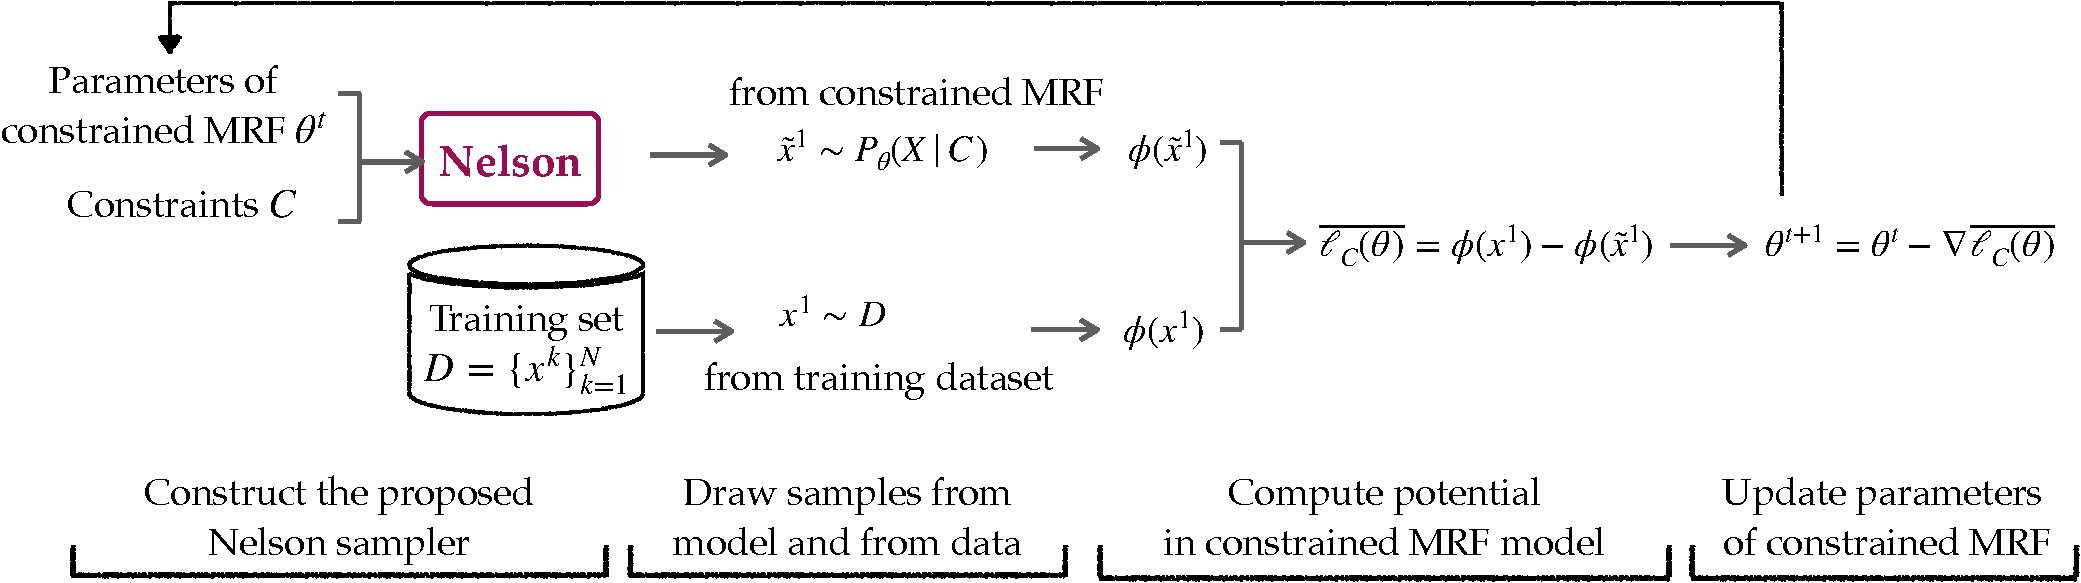
\includegraphics[width=0.99\linewidth]{figs/learn-pipeline-crop.pdf}
    \captionof{figure}{Implementation pipeline of the \nls-CD algorithm with $m=1$. The proposed \nls can be efficiently adapted to a PyTorch-based machine learning library and enforces constraint satisfaction during learning.}\label{fig:pipeline}
\end{figure*}

\subsubsection*{Implementation of  Algorithm~\ref{alg:main}}  We first use the Constraints $\mathcal{C}$ and parameters $\theta^t$ to build the current \nls module.  Then we draw $m$ samples from \nls module $\{\tilde{x}^j\}_{j=1}^m$ and draw from dataset randomly $m$ samples $\{x^j\}_{j=1}^m$. Continuing from that point, we compute the potential value from the two sets of inputs, i.e., $\{ \phi_{\theta}(\tilde{x}^j)\}_{j=1}^m$ and $\{ \phi_{\theta}(x^j)\}_{j=1}^m$. PyTorch would be slow if we compute each potential's gradient using a for-loop. To bypass this problem, we instead compute the following:
\begin{equation} \label{eq:emp-gradient}
    \overline{\ell_{\mathcal{C}}(\theta)}= \frac{1}{m}\sum_{j=1}^m \phi_{\theta}(x^j)-\frac{1}{m}\sum_{j=1}^m \phi_{\theta}(\tilde{x}^j).
\end{equation}
Following that, we call the PyTorch library's gradient function, which computes exactly
\begin{equation*}
    \begin{aligned}
        \nabla\overline{\ell_{\mathcal{C}}(\theta)} & =\nabla\left(\frac{1}{m}\sum_{j=1}^m \phi_{\theta}(x^j)-\frac{1}{m}\sum_{j=1}^m \phi_{\theta}(\tilde{x}^j)\right)=\frac{1}{m}\sum_{j=1}^m \nabla\phi_{\theta}(x^j)-\frac{1}{m}\sum_{j=1}^m \nabla\phi_{\theta}(\tilde{x}^j)
    \end{aligned}
\end{equation*}
Note that $\nabla\overline{\ell_{\mathcal{C}}(\theta)}$ recovers the result in Equation~\eqref{eq:gradient}. Finally, we update the parameters $\theta$. The proposed \nls module and the neural network are computed on the same GPU device. This allows us to exploit the parallel computing power of modern GPUs and remove time for the data transfer from CPU to GPU or vice versa.   See Figure~\ref{fig:pipeline} for a visualized overview of the implementation with PyTorch.

\subsection{Learn Random K-SAT Solutions with Preference}
\subsubsection*{Task Definition}  We are given a training set $\mathcal{D}$ containing some preferred assignments
$\mathcal{D}=\{x^j\}_{j=1}^N$ for the corresponding CNF formula
$c_1\wedge\ldots\wedge c_L$. We require the CNF formula to be true. This means,
by the definition of CNF formulas, that every clause has to be satisfied. These
clauses become our set of constraints. Under the constrained MRF model, the
learning task is to maximize the log-likelihood of the assignments seen in the
training set $\mathcal{D}$. The inference task is to generate valid solutions
from the learned model's
distribution~\citep{DBLP:conf/aiia/DodaroP19,DBLP:conf/sac/RosaGO11}.

%

\subsubsection*{Dataset} We denote the Boolean variables' size in $K$-SAT as the ``problem size''. We
consider several datasets of different problem sizes generated from
CNFGen\footnote{\url{https://github.com/MassimoLauria/cnfgen}}~\citep{DBLP:conf/sat/LauriaENV17}
random $K$-SAT functions. $K$ is fixed as $5$; the numbers of variables and
clauses are kept the same, ranging from $10$ to $1500$. We generate $100$
different CNF formulas for every problem size. To generate the training set
$\mathcal{D}$, we use the Glucose4 solver from
PySAT\footnote{\url{https://pysathq.github.io/}}
library~\citep{DBLP:conf/sat/IgnatievMM18} to generate $200$ assignments
randomly as the preferred assignments for every formula.

It should be pointed out that we don't consider datasets like SATLIB and SAT
competitions. It is mainly because these datasets are hard instances with a
much larger input space but a limited number of solutions. \nls would generally
take exponential time to find these solutions, just like finding needles in a
haystack. Another reason is that using neural networks to learn these
limited assignments is straightforward since we can simply hard-wire the
network to memorize all the valid assignments. The main purpose of this work is
to let a constrained MRF learn a representation for the underlying preference
pattern, not create a neural solver that can generate valid assignments for any
CNF formula. Thus, we conform to the settings of the easy formula where
obtaining valid solutions is easy.

\subsection{Learn Sink-Free Orientation in Undirected Graphs}
\textbf{Task Definition} In graph theory, a \textit{sink-free} orientation of an undirected graph is a choice of orientation for each edge such that every vertex has at least one outgoing edge~\citep{DBLP:journals/combinatorics/CohnPP02}. It has wide applications in robotics routing and IoT network configuration~\citep{takahashi2009communication}.  The Constraints for this problem are that every vertex has at least one outgoing edge after orientation. As stated in~\citep{DBLP:journals/jacm/GuoJL19}, these constraints satisfy Condition~\ref{cond:extreme}.

{See Figure~\ref{fig:sinkfreeex} for an example graph and one possible sink-free edge orientation. We define binary variables $X_1,\ldots, X_m$, and associate variable $X_i$ to edge $e_i$ for $1\le i\le m$. Variable $X_i$ takes value $1$ if the edge orientation is $v_i\to v_j$ where $i<j$. Otherwise, $X_i$ takes value $0$. The constraints are:}
\begin{equation*}
    \mathcal{C}=(X_1\vee X_2)\wedge(\neg X_1\vee X_3\vee\neg X_4)\wedge(\neg X_2\vee\neg X_3\vee X_5)\wedge(X_4\vee \neg X_5)
\end{equation*}
{where the single constraint  $c_1=(X_1\vee X_2)$ corresponds to vertex $v_1$, constraint $c_2=(\neg X_1\vee X_3\vee\neg X_4)$ corresponds to vertex  $v_2$, constraint $c_3=(\neg X_2\vee\neg X_3\vee X_5)$  corresponds to vertex  $v_3$, and constraint $c_4=(X_4\vee \neg X_5)$ corresponds to vertex  $v_4$. The orientation assignment matrix $x$ shown in Figure~\ref{fig:sinkfreeex}(b) implies: $X_1=1,X_2=1,X_3=1,X_4=0,X_5=1$.}

\begin{figure}[t]
    \centering
    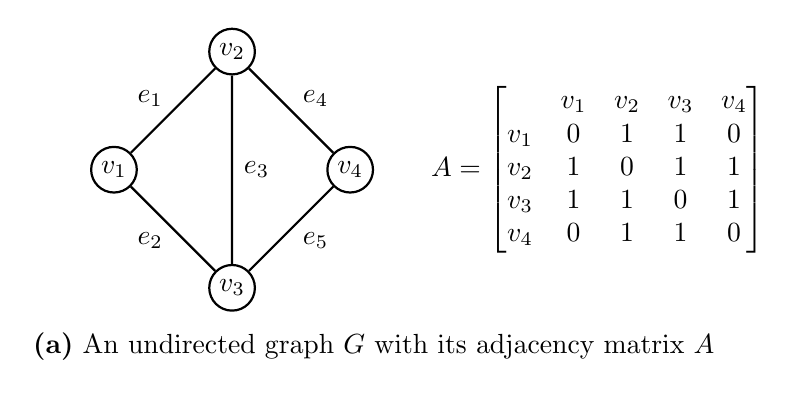
\begin{tikzpicture}[xscale=0.15, yscale=0.15, inner sep=2pt, >=stealth]
        \draw (-5,10)  node[circle,thick,draw] (v1) {$v_1$};
        \draw (5,20) node[circle,thick,draw] (v2) {$v_2$};
        \draw (5,0)  node[circle,thick,draw] (v3) {$v_3$};
        \draw (17,-5) node[thick] (v4) {\textbf{(a)} An undirected graph $G$ with its adjacency matrix $A$};
        \draw (15,10) node[circle,thick,draw] (v4) {$v_4$};
        \draw (36,10)  node (v5) {$A=\begin{bNiceMatrix}[
                        %   first-row,code-for-first-row=\normalsize,
                        %   first-col,code-for-first-col=\normalsize,
                    ]
                        & v_1 & v_2 & v_3 & v_4 \\
                    v_1 & 0   & 1   & 1   & 0   \\
                    v_2 & 1   & 0   & 1   & 1   \\
                    v_3 & 1   & 1   & 0   & 1   \\
                    v_4 & 0   & 1   & 1   & 0   \\
                \end{bNiceMatrix}$};
        \draw[-,thick] (v1) -- (v2);
        \draw[-,thick] (v1) -- (v3);
        \draw[-,thick] (v2) -- (v3);
        \draw[-,thick] (v4) -- (v2);
        \draw[-,thick] (v3) -- (v4);
        \draw (-1,16)  node[text width = 6mm] () {$e_1$};
        \draw (-1,4)   node[text width = 6mm] () {$e_2$};
        \draw (8,10) node[text width = 6mm] () {$e_3$};
        \draw (13,16) node[text width = 6mm] () {$e_4$};
        \draw (13,4)  node[text width = 6mm] () {$e_5$};
    \end{tikzpicture}
    \hfill
    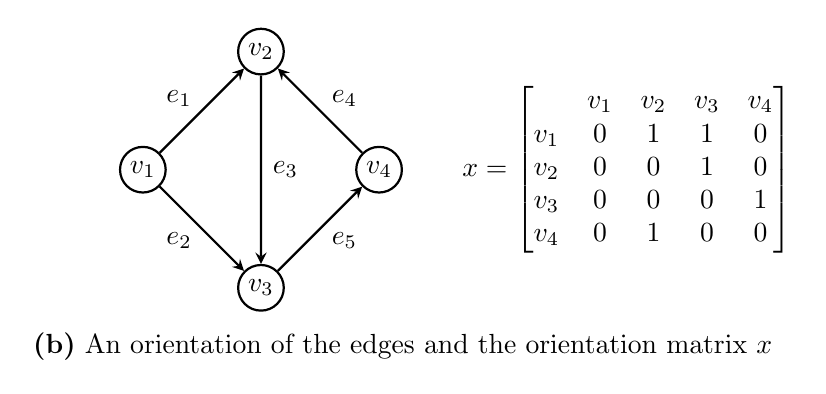
\begin{tikzpicture}[xscale=0.15, yscale=0.15, inner sep=2pt, >=stealth]
        \draw (-5,10)  node[circle,thick,draw] (v1) {$v_1$};
        \draw (5,20) node[circle,thick,draw] (v2) {$v_2$};
        \draw (5,0)  node[circle,thick,draw] (v3) {$v_3$};
        \draw (17,-5) node[thick] (v4) {\textbf{(b)} An orientation of the edges and the orientation matrix $x$};
        \draw (15,10) node[circle,thick,draw] (v4) {$v_4$};
        \draw (36,10)  node (v5) {$x=\begin{bNiceMatrix}[
                        %   first-row,code-for-first-row=\normalsize,
                        %   first-col,code-for-first-col=\normalsize,
                    ]
                        & v_1 & v_2 & v_3 & v_4 \\
                    v_1 & 0   & 1   & 1   & 0   \\
                    v_2 & 0   & 0   & 1   & 0   \\
                    v_3 & 0   & 0   & 0   & 1   \\
                    v_4 & 0   & 1   & 0   & 0   \\
                \end{bNiceMatrix}$};
        \draw[->,thick] (v1) -- (v2);
        \draw[->,thick] (v1) -- (v3);
        \draw[->,thick] (v2) -- (v3);
        \draw[->,thick] (v4) -- (v2);
        \draw[->,thick] (v3) -- (v4);
        \draw (-1,16)  node[text width = 6mm] () {$e_1$};
        \draw (-1,4)   node[text width = 6mm] () {$e_2$};
        \draw (8,10) node[text width = 6mm] () {$e_3$};
        \draw (13,16) node[text width = 6mm] () {$e_4$};
        \draw (13,4)  node[text width = 6mm] () {$e_5$};
    \end{tikzpicture}
    \caption{{\textbf{(a)} An un-directed graph $G(V,E)$ where the vertices are $V=\{v_1,v_2,v_3,v_4\}$ and the un-directed edges are $E=\{e_1=(v_1,v_2),e_2=(v_1,v_3),e_3=(v_2,v_3),e_4=(v_2,v_4),e_5=(v_3,v_4)\}$. \textbf{(b)} A possible sink-free orientation of the edges in the graph and its matrix representation $x$, where every vertex has at least one outgoing edge. }}
    \label{fig:sinkfreeex}
\end{figure}

\subsubsection*{Notations} Let graph $G(V,E)$ be an un-directed graph; its adjacency matrix $A$ that
represents graph connectivity is:
\begin{equation}\label{eq:adjacency}
    A_{ij}=\begin{cases}
        {1} & \text{If } (v_i,v_j)\in E \\
        0   & \text{otherwise}
    \end{cases}
\end{equation}
A possible assignment for the orientation of every edge can be represented as a matrix $x\in\{0,1\}^{|V|\times |V|}$:
\begin{equation}\label{eq:orientation-assign}
    x_{ij}=\begin{cases}
        1 & \text{if the edge orientation is } v_i\to v_j \\
        0 & \text{otherwise}
    \end{cases}
\end{equation}
In the constrained MRF model defined in Eq.~\eqref{eq:constr_mrf_single}, the potential function of one orientation of all edges is
\begin{equation*}
    \phi_{\theta}(x)=\sum_{i=1}^{|V|}\sum_{j=1}^{|V|}\theta_{ij}A_{ij}x_{ij}
\end{equation*}
A single constraint for vertex $v_k$ is $c_k(x)=\mathbf{1}\left(\sum_{j=1}^{|V|}A_{k,j}x_{k,j}\ge1\right)$. It equals zero if there is no outgoing edge from vertex $v_k$. The constraint function is $C(x)=\prod_{k=1}^{|V|}c_k(x)$. In Algorithm~\ref{alg:lll-sampler} step 1, edge $(v_i,v_j)$ will pick the orientation $v_i\to v_j$  with probability:
\begin{equation*}
    \frac{\exp(\theta_{ij}A_{ij}x_{ij})}{\exp(\theta_{ji}A_{ji}x_{ji})+\exp(\theta_{ij}A_{ij}x_{ij})}
\end{equation*}

\subsubsection*{Dataset} {We use the NetworkX\footnote{https://networkx.org/} package to generate random Erd\H{o}s-R\'enyi graphs with edge probability $0.55$. The problem size refers to the number of vertices in the graph, we range the problem size from 10 to 100. For each problem size, we generate 100 different random undirected graphs. We then convert the graph into CNF form using the above edge-variable conversion rule. Afterward, we follow the same processing steps as the previous problem that learns preferential solution distribution for random K-SAT. }

%

\subsection{Learn Vehicle Delivery Routes}
Given a set of locations to visit, the task is to generate a sequence to visit
these locations in which each location is visited once and only once and the
sequence closely resembles the trend presented in the training data. The
training data are such routes collected in the past. The dataset is constructed
from TSPLIB, which consists of $29$ cities in Bavaria, Germany.
%
In Figure~\ref{fig:route}, we see \nls can obtain samples of this delivery
problem highly efficiently. %

A possible travel plan can be represented as a matrix $x\in\{0,1\}^{|V|\times
    |V|}$:
\begin{equation}\label{eq:route}
    x_{ij}=\begin{cases}
        1 & \text{if edge } v_i\to v_j \text{ is selected} \\
        0 & \text{otherwise}
    \end{cases}
\end{equation}
The constraints are that every  routing plan should visit every location once and only once.

Similarly, in the constrained MRF model defined in
Eq.~\eqref{eq:constr_mrf_single}, the potential function of the vehicle routing
plan is
\begin{equation*}
    \phi_{\theta}(x)=\sum_{i=1}^{|V|}\sum_{j=1}^{|V|}\theta_{ij}A_{ij}x_{ij}
\end{equation*}

%

\subsection{Detailed Baselines Configuration}
In terms of sampling-based methods, we consider:
\begin{itemize}
    \item Gibbs sampler~\citep{carter1994gibbs}, a special case of MCMC that is widely
          used in training MRF models. In each step, the Gibbs algorithm samples one
          dimension based on a conditional marginal distribution. We follow this
          implementation\footnote{\url{https://github.com/Fading0924/BPChain-CD/blob/master/mrf.py}}.
    \item Weighted SAT samplers, including
          WAPS\footnote{\url{https://github.com/meelgroup/waps}}~\citep{DBLP:conf/tacas/GuptaSRM19},
          WeightGen\footnote{\url{https://bitbucket.org/kuldeepmeel/weightgen/src/master/}},
          ~\citep{DBLP:conf/aaai/ChakrabortyFMSV14} and XOR
          sampler\footnote{\url{https://cs.stanford.edu/~ermon/code/srcPAWS.zip}}~\citep{DBLP:conf/nips/ErmonGSS13,DBLP:conf/uai/DingX21}.
    \item Uniform SAT samplers, including
          UniGen\footnote{\url{https://github.com/meelgroup/unigen}},~\citep{DBLP:conf/cav/SoosGM20},
          QuickSampler\footnote{\url{https://github.com/RafaelTupynamba/quicksampler}},
          ~\citep{DBLP:conf/icse/DutraLBS18},
          CMSGen\footnote{\url{https://github.com/meelgroup/cmsgen}}~\citep{DBLP:conf/fmcad/GoliaSCM21}
          and
          KUS\footnote{\url{https://github.com/meelgroup/KUS}}~\citep{DBLP:conf/lpar/SharmaGRM18}.
\end{itemize}
Currently, there are only GPU-based SAT solvers~\citep{DBLP:conf/sat/PrevotSM21,mahmoud2022gpu} and model counters~\citep{DBLP:conf/cp/FichteHZ19}; GPU-based SAT samplers are not available so far.

\subsection{Detailed Definition of Evaluation Metrics}
In terms of evaluation metrics, we consider
\begin{itemize}
    \item Training time per epoch. The average time for the whole learning method to
          finish one epoch with each sampler.
    \item Validness. The learned model is adopted to generate assignments and we evaluate
          the percentage of generated assignments that satisfy the constraints.
    \item  Mean Averaged Precision (MAP$@10$). This is a ranking-oriented metric that can
          evaluate the closeness of the learned MRF distribution to the goal
          distribution. If the model learns the goal distribution in the training set,
          then it would assign a higher potential value to those assignments in the
          training set than all the rest of the unseen assignments. Based on this principle, we
          randomly pick two sets of inputs in those valid assignments: seen assignments
          from the training set and unseen assignments that are randomly generated. We
          use the value of factor potential $\phi(x)$ to rank those assignments in
          ascending order. Next, we check how many preferred solutions can fall into the
          Top-$10$ by computing the following
          \begin{equation*}
              \text{MAP}@10=\sum_{k=1}^{10}\frac{\#\text{preferred assignments among top-} k}{k}
          \end{equation*}

    \item $\log$-likelihood of assignments in the training set $\mathcal{D}$. The model that attains the highest $\log$-likelihood learns the closest  distribution to the training set.  Specifically, given a training set $\mathcal{D}=\{x^k\}_{k=1}^N$ and parameters $\theta$, the log-likelihood value is:
          \begin{equation}
              \begin{aligned}
                  {\frac{1}{N}\sum_{k=1}^N\log P_{\theta}(X=x^k|\mathcal{C})} & =\frac{1}{N}\sum_{k=1}^N\phi_\theta(x^k)- \log Z_\mathcal{C}(\theta)
              \end{aligned}
          \end{equation}
          We use the ACE algorithm to compute the approximated value of $\log Z_\mathcal{C}(\theta) $\footnote{\url{http://reasoning.cs.ucla.edu/ace/moreInformation.html}}.

    \item Approximation Error of $\nabla \log Z_{\mathcal{C}}(\theta)$, that is the $L_1$
          distance between the exact gradient of $ \log Z_{\mathcal{C}}(\theta)$ in
          Eq.~\eqref{eq:gradient} and the empirical gradient from the sampler. For small
          problem sizes, we enumerate all $x\in \mathcal{X}$ to get the exact gradient
          and draw samples $\{\tilde{x}^j\}_{j=1}^m$ with $m=2000$ from every sampler for
          approximation.
          \begin{equation*}
              \left|\, \, \underbrace{\sum_{x\in\mathcal{X}} \frac{\exp\left( \sum_{j=1}^n\theta_jx_j\right)C(x) }{Z_\mathcal{C}(\theta)}{x_i}}_{\text{{Exact gradient term}}} \ - \ \underbrace{\sum_{j=1}^m \tilde{x}^j_i}_{\text{{Estimated gradient with sampler}}} \, \,\right|
          \end{equation*}
          For fixed parameter $\theta$, the best sampler would attain the smallest approximation error.
\end{itemize}

\subsection{Hyper-parameter Settings}
In the implementation of \nls, we set the maximum tryout of resampling as
$T_{tryout}=1000$ for all the experiments and all the datasets.

For the hyper-parameters used in learning the constrained MRF, we set the
number of samples from the model to be $m=200$, the learning rate $\eta$ is
configured as $0.1$ and the total learning iterations are $T_{\max}=1000$.

\begin{figure*}[!ht]
    \centering
    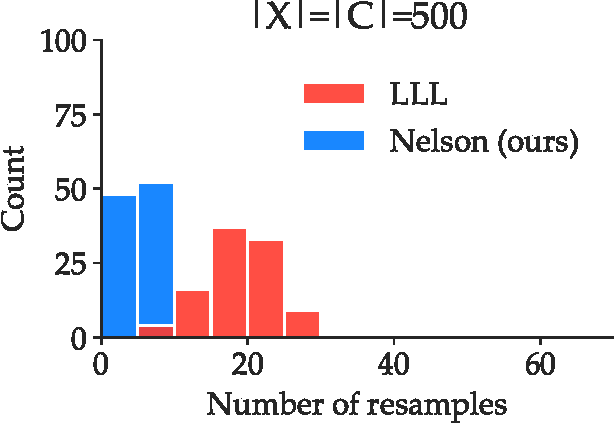
\includegraphics[width=0.245\linewidth]{exp/randkcnf_5_500_500_0001.uniform.pdf}
    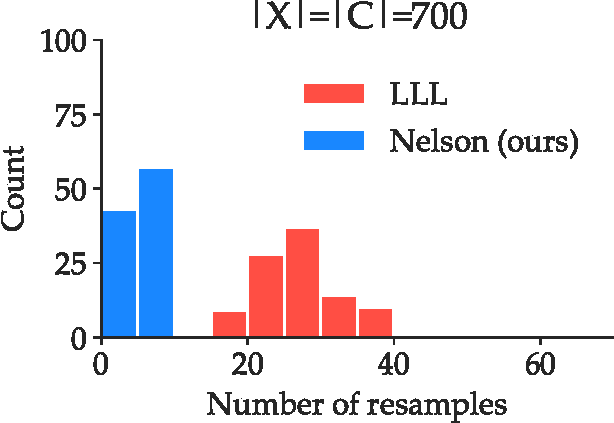
\includegraphics[width=0.245\linewidth]{exp/randkcnf_5_700_700_0001.uniform.pdf}
    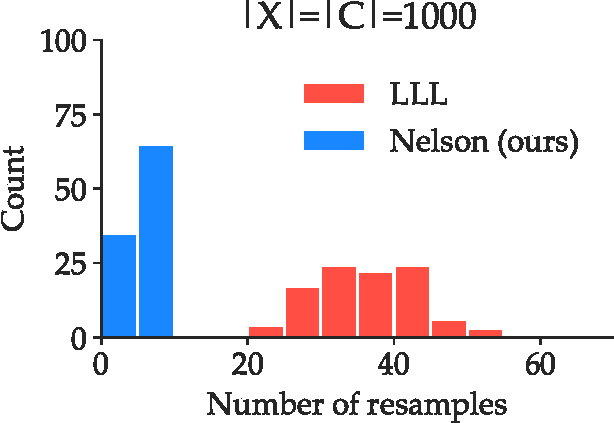
\includegraphics[width=0.245\linewidth]{exp/randkcnf_5_1000_1000_0001.uniform.pdf}
    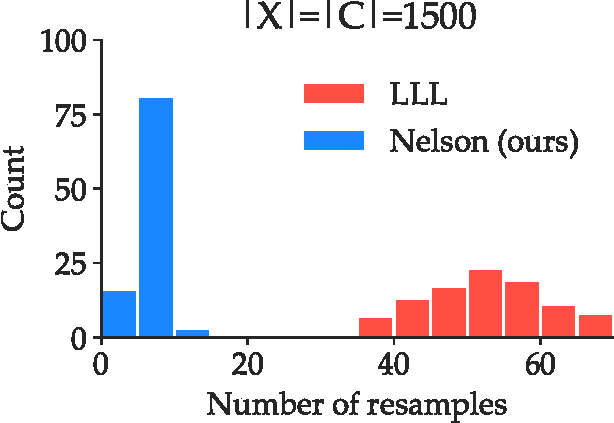
\includegraphics[width=0.245\linewidth]{exp/randkcnf_5_1500_1500_0001.uniform.pdf}
    \begin{center}
        (a) Uniform Case.
    \end{center}
    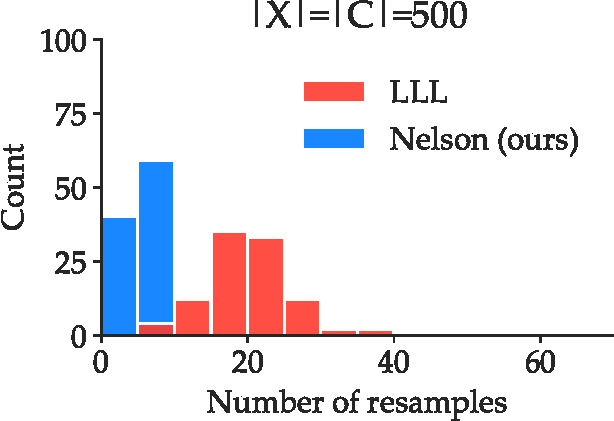
\includegraphics[width=0.245\linewidth]{exp/randkcnf_5_500_500_0001.weighted.pdf}
    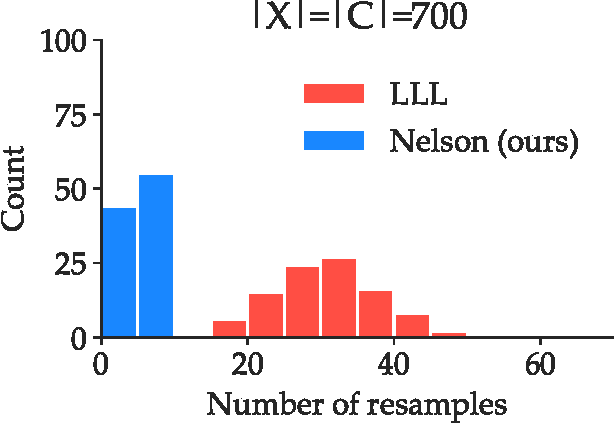
\includegraphics[width=0.245\linewidth]{exp/randkcnf_5_700_700_0001.weighted.pdf}
    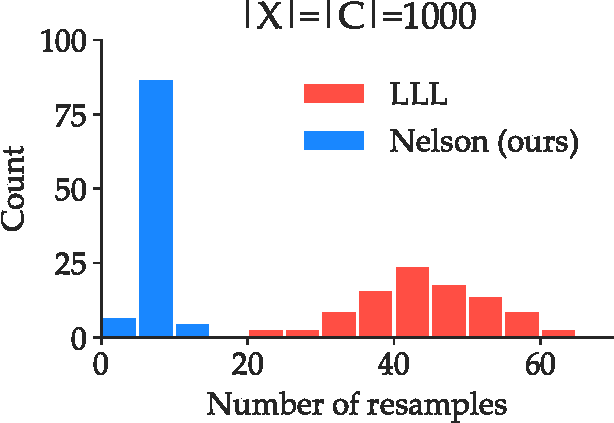
\includegraphics[width=0.245\linewidth]{exp/randkcnf_5_1000_1000_0001.weighted.pdf}
    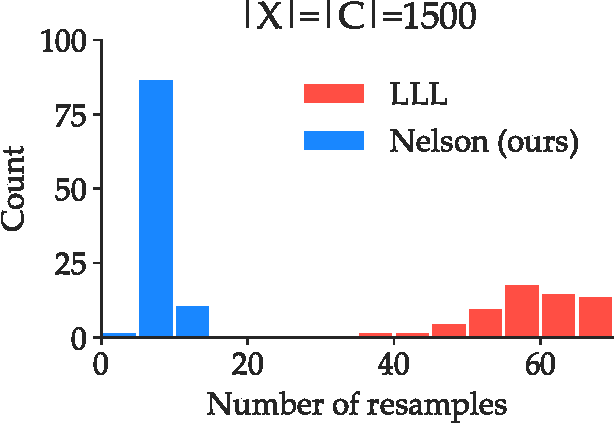
\includegraphics[width=0.245\linewidth]{exp/randkcnf_5_1500_1500_0001.weighted.pdf}
    \begin{center}
        (b) Weighted Case.
    \end{center}
    \caption{The distribution of resampling steps in the \nls and Algorithmic-LLL~\citep{DBLP:journals/jacm/MoserT10}. Both of them get a valid sample within $T_{\mathit{tryouts}}$. \nls takes far fewer resamples than Algorithmic-LLL because it resamples all the violated clauses at every iteration while Algorithmic-LLL only resamples one of them.}\label{fig:ap:resamples}
\end{figure*}


\chapter{VarFA: A Variational Factor Analysis Framework For Efficient Bayesian Learning Analytics}
\nnfootnote{Published in EDM 2020.}
\section*{Overview}
In the last chapter of this thesis, we propose VarFA, a variational inference factor analysis framework that extends existing factor analysis models for educational data mining to efficiently output uncertainty estimation in the model's estimated factors. Such uncertainty information is useful, for example, for an adaptive testing scenario, where additional tests can be administered if the model is not quite certain about a students' skill level estimation. Traditional Bayesian inference methods that produce such uncertainty information are computationally expensive and do not scale to large data sets. VarFA utilizes variational inference which makes it possible to efficiently perform Bayesian inference even on very large data sets. We use the sparse factor analysis model as a case study and demonstrate the efficacy of VarFA on both synthetic and real data sets. VarFA is also very general and can be applied to a wide array of factor analysis models. Code and instructions to reproduce results in this chapter are available from~{\color{blue}{\url{https://tinyurl.com/tvm4332}}}.
\section{Introduction}
\label{sec:intro}
%
A core task for many practical educational systems is \textit{student
    modeling}, i.e., estimating students' mastery level on a set of skills or
knowledge components (KC)~\cite{vanlehn1988student, chrysafiadi2013student}.
Such estimates allow in-depth understanding of students' learning status and
form the foundation for automatic, intelligent learning interventions. For
example, intelligent tutoring systems (ITSs)~\cite{shute1994intelligent,
    pls1,anderson1995cognitive,nye2014autotutor,heffernan2014assistments,rafferty2015inferring}
rely on knowing the students' skill levels in order to effectively recommend
individualized learning curriculum and improve students' learning outcomes. In
the big data era, student modeling is usually formulated as an educational data
mining (EDM)
problem~\cite{romero2010educational,baker2009state,merceron2005educational}
where an underlying machine learning (ML) model estimates students' skill
mastery levels from students' learning records, i.e., their answers to
assessment questions.

\sloppy
Many student modeling methods have been proposed in prior literature. A fruitful line of research for student modeling follows the \textit{factor analysis (FA)} approach.
FA models usually assume that an unknown, potentially multi-dimensional student parameter, in which each dimension is associated with a certain skill, explains how a student answers questions and is to be estimated. Popular and successful FA models include item response theory (IRT)~\cite{irt}, multi-dimensional IRT~\cite{mirt}, learning factor analysis (LFA)~\cite{LFA}, performance factor analysis (PFA)~\cite{PFA}, DASH (short for {d}ifficulty, {a}bility, and {s}tudent {h}istory)~\cite{lindsey2014improving,mozer2016predicting}, DAS3H (short for {d}ifficulty, {a}bility, {s}kill and {s}tudent {s}kill {h}istory)~\cite{das3h}, knowledge tracing machines (KTM)~\cite{vie2019knowledge}, and so on.
% 
Recently, more complex student models based on deep neural networks (DNN) have
also been proposed~\cite{DKT,zhang2017dynamic,minn2018deep}. Nevertheless,
thanks to their simplicity, effectiveness and robustness, FA models remain
widely adopted and investigated for practical EDM tasks. Moreover, there is
evidence that simple FA models could even outperform DNN models for student
modeling in terms of predicting students' answers~\cite{irt-best}. Because of
FA models' competitive performance and its elegant mathematical form, we focus
on FA-based student models in this chapter.

Most of the aforementioned FA models compute a single point estimate of skill
levels for each student. Often, however, it is not enough to obtain mere point
estimates of students' skill levels; knowing the model's uncertainty in its
estimation is crucial because it potentially helps improve the model's
performance and improve both students' and instructors' experience with
educational systems.
% 
For example, in ITS, an underlying model can use the uncertainty information in
its estimation of students' skill level to automatically decide that its
recommendations based on highly uncertain estimations are unreliable and
instead notify a human instructor to evaluate the students' performance. This
enables collaboration between ITS and instructors to create a more effective
learning environment.
%
In adaptive testing systems~\cite{chang2009nonlinear,yan2016computerized},
knowing the uncertainty in model's estimation could help the model
intelligently pick the next test items to most effectively reduce its
uncertainty about estimated students' skill levels. This will help to
potentially reduce the number of items needed to have a confident, accurate
estimation of the students' skill mastery level, saving time for both students
to take the test and instructors to have a good assessment of the student's
skills.

All the above applications require the model to ``know what it does not know,''
i.e., to quantify the uncertainty of its estimation. Achieving this does not
necessary changes the model. rather, we need a different inference algorithm
for inferring not only a point estimate of student's skill level from observed
data (i.e., students' answer records to questions) but also uncertainty in the
estimations.

Fortunately, there exist methods that both compute point estimates of students'
skill levels and quantifies the uncertainty of those estimates. These methods
usually follow the Bayesian inference paradigm, where each student's unknown
skill levels are treated as random variables drawn from a \textit{posterior
    distribution}. Thus, one can use the \textit{credible interval} to quantify the
model's uncertainty on the student's estimated skill level. A classical method
for Bayesian inference is Monte Carlo Markov Chain (MCMC)
sampling~\cite{gelman2013bayesian} which has been widely used in many other
disciplines~\cite{gilks1995markov} other than EDM. In the context of student
modeling with FA models, existing works such as
~\cite{lan14a,fox2010bayesian,pardos2010using,merkle2011comparison} have
applied MCMC methods to obtain credible intervals.

Unfortunately, classic Bayesian inference methods suffer from extensive
computational complexity. For example, each computation step in MCMC involves a
time-consuming evaluation of the posterior distribution. Making matters worse,
MCMC typically takes many more steps to converge than non-Bayesian inference
methods. As a concrete illustration, in~\cite{lan14a}, the Bayesian inference
method (10 minutes) is about 100 times slower than the other non-Bayesian
inference method based on stochastic gradient descent (6 seconds). The high
computational cost prevents Bayesian inference methods from mass-deployment in
large-scale, real-time educational systems where timely feedback is critical
for learning~\cite{driscoll1994psychology} and tens of thousands of data points
need to be processed in seconds or less instead of minutes or hours. It is thus
highly desirable to accelerate Bayesian inference so that one can quantify
model's uncertainty in its estimation as efficiently as non-Bayesian inference
methods.
%

\subsubsection*{Contributions}
In this work, we propose VarFA, a novel framework based on \textit{variational
    inference} (VI) to perform efficient, scalable Bayesian inference for FA
models. The key idea is to approximate the true posterior distribution, whose
costly computation slows down Bayesian inference, with a \textit{variational
    distribution}. We will see in Section~\ref{sec:method} that, with this
approximation, we turn Bayesian inference into an optimization problem where we
can use the same efficient inference algorithms as in non-Bayesian inference
methods. Moreover, the variational distribution is very flexible and we have
full control specifying it, allowing us to freely use the latest development in
machine learning, e.g., deep neural networks (DNNs), to design the variational
distribution that closely approximates the true posterior. Thus, we also regard
our work as a first step in applying DNNs to FA models for student modeling,
achieving efficient Bayesian inference (enabled by DNNs) without losing
interpretability (brough by FA models).
%
We demonstrate the efficacy of our framework on both synthetic and real data
sets, showcasing that VarFA substantially accelerates classic Bayesian
inference for FA models with no compromise on performance.
%

The remainder of this chapter is organized as follows.
Section~\ref{sec:related-work} introduces the problem setup in FA and reviews
the important FA models and their inference methods, in particular Bayesian
inference. Section~\ref{sec:method} explains our VarFA framework in detail.
Section~\ref{sec:experiments} presents extensive experimental results that
substantiate the claimed advantages of our framework.
Section~\ref{sec:conclusion} concludes this chapter and discusses possible
extensions to VarFA.

\section{Background and Related Work}
\label{sec:related-work}
We first set up the problem and review related work. Assume we have a data set $\mY\in\mathbb{R}^{N\times Q}$ organized in matrix format where $N$ is the total number of students and $Q$ is the number of questions. This is a binary students' answer record matrix where each entry $y_{ij}$ represents whether student $i$ correctly answered question $j$. Usually, not all students answer all questions. Thus, $\mY$ contains missing values. We use $\{i,j\}\in\Omega_{\rm obs}$ to denote entries in $\mY$, i.e., the $i$-th student's answer record to the $j$-th question, that are observed.

We are interested in models capable of inferring each $i$-th student's skill
mastery level that can accurately predict the student's answers given the above
data. These models are often evaluated on the prediction accuracy and whether
the inferred student skill mastery levels are easily interpretable and
educationally meaningful. We now review factor analysis models (FA), one of the
most widely adopted and successful methodologies for the student modeling task.

\subsection{Factor Analysis For Student Modeling}
\label{sec:fa}
% 
One of the earliest FA model for student modeling is based on the item response
theory (IRT)~\cite{irt}. It usually has the following form
\begin{align}
    \begin{split}
        \mathbb{P}(y_{ij}=1) = \sigmoid(c_i + \mu_j)\,,\label{eq:irt}
    \end{split}
\end{align}
which assumes that each student's answer $y_{ij}$ is independently Bernoulli distributed. The above formula says that the students' answers can be explained by an unknown scalar student skill level factor $c_i$ for each student $i$ and an unknown scalar question difficulty level factor $\mu_j$ for each question $j$. $\sigmoid(\cdot)$ is a Sigmoid activation function, i.e., $\sigmoid(x) = 1 / (1 + {\rm exp}(-x))$. The multi-dimensional IRT model (MIRT)~\cite{mirt} extends IRT by using a multi-dimensional vector to represent the student skill levels. More recently,~\cite{lan14a} proposed sparse factor analysis model (SPARFA) which extends MIRT by imposing additional assumptions, resulting in improved interpretations of the inferred factors.

Other FA models seek to improve student modeling performance by cleverly
incorporate additional auxiliary information.
% One form of such auxiliary information is the skill tags associated with each question (recall this is assumed to be unknown in, e.g., SPARFA). This question-skill association information is commonly known as the $Q$ matrix in literature [CITE]. Another form of auxiliary information is the accumulative history answer records of students, i.e., the total count of correct or incorrect answers for a question. 
For example, the additive factor model (AFM)~\cite{LFA} incorporates students'
accumulative correct answers for a question and the skill tags associated with
each question:
\begin{align}
    \begin{split}
        \mathbb{P}(y_{ij}=1) = \sigmoid\left(c_i + \sum_{k=1}^\kappa\big( q_{kj}\beta_k + q_{kj}\rho_k b_{ik} \big)\right)\,,\label{eq:laf}
    \end{split}
\end{align}
where $\kappa$ is the total number of skills in the data, $b_{ik}$ is the $i$-th student's total number of correct answers for skill $k$ and $q_{kj}\in\{0,1\}$ indicates whether the skill $k$ is associated with question $j$. In particular, $q_{kj}$'s form matrix $\mQ\in\mathbb{R}^{K\times Q}$ which is commonly known as the Q-matrix in literature~\cite{qmatrix}. The unknown, to-be-inferred factors are $\beta_k$, a scalar difficulty factor for each skill $k$, and $\rho_k$, a scalar learning rate of skill $k$.
%
The performance factor model (PFM)~\cite{PFA} builds upon AFM that additionally
incorporate the total number of a student's incorrect answers to questions
associated with a skill. The instructor factor model
(IFM)~\cite{chi2011instructional} further builds on PFM to incorporate the
prior knowledge of whether a student has already mastered a skill. More
recently, ~\cite{vie2019knowledge} introduces knowledge tracing machines (KTM)
that could flexibly incorporate a number of auxiliary information mentioned
above, thus generalizing AFM, PFM and IFM.

Another way to improve student modeling performance is to utilize the so-called
\textit{memory}, i.e., using students' historic action data over time. For
example, ~\cite{lindsey2014improving,mozer2016predicting} proposed DASH (short
for \underline{d}ifficulty, \underline{a}bility, and \underline{s}tudent
\underline{h}istory) that incorporates a student's total number of correct
answers and total number of attempts for a question in a given time window
\begin{align} \label{eq:dash}
    \mathbb{P}(y_{ij}=1)  = \sigmoid\Bigg( c_i - \mu_j + \sum_{w=0}^{W-1} \Big(\theta_{2w+1}{\rm log}(1+\rho_{ijw}) - \theta_{2w+2}{\rm log}(1+\gamma_{ijw})\Big) \Bigg)
\end{align}
where $W$ is the length of the time windows (e.g., number of days), $\rho_{ijw}$ and $\gamma_{ijw}$ are the $i$-th student's total number of correct answers and total number of attempts for question $j$ at time $w$, respectively. $\theta$'s are parameters that captures the effect of correct answers and total attempts. More recently, DAS3H~\cite{das3h} extends DASH to further include skill tags associated with each question which essentially amounts to adding, within the last summation term in Eq.~\ref{eq:dash}, another summation over the number of skills.

\subsubsection{A general formulation for FA models}
Although the above FA models differ in their formulae, modeling assumptions and
the available auxiliary data used, we argue that the aforementioned FA models
can be unified into a canonical formulation below
\begin{align}
    \begin{split}
        \mathbb{P}(y_{ij}=1) = \sigmoid(\rvc_i^\top \rvm_j + \mu_j)\,, \label{eq:sparfa}
    \end{split}
\end{align}
where $\rvc_i\in\mathbb{R}^K$, $\rvm_j\in\mathbb{R}^K$ and $\mu_j\in\mathbb{R}$ are factors whose dimension, interpretations and subscript indices depend on the specific instantiations of the FA model. To illustrate that Eq.~\ref{eq:sparfa} subsumes the FA models mentioned above, we demonstrate, as examples, how to turn SPARFA and AFM into the form in Eq.~\ref{eq:sparfa} and how to reinterpret the parameters in the reformulation. The equivalence between Eq.~\ref{eq:sparfa} and the original SPARFA formula is immediate and we can interpret the parameters in Eq.~\ref{eq:sparfa} as follows to recover SPARFA: $K$ is the number of \textit{latent skills} that group the actual skill tags in the data set into meaningful coarse clusters; $\rvc_i$ represents the $i$-th student's skill level on the latent skills; $\rvm_j$ represents the strength of association of the $j$-th question with the latent skills which is assumed to be nonnegative and sparse for improved interpretation; and $\mu_j$ represents the difficulty of question $j$. All three factors in SPARFA are assumed to be unknown.

Similarly, for AFM, we can perform the following change of variables and
indices to obtain Eq.~\ref{eq:sparfa}. We first change the indices $\rvm_j$ to
$\rvm_{ij}$ and $\mu_j$ to $\mu_i$, and remove the index in $\rvc_i$ to $\rvc$.
Then, we simply set $\rvc = [\beta_1, ..., \beta_\kappa, \rho_1, ...,
    \rho_\kappa]^\top$, $\rvm_{ij} = [q_{1j},...,q_{\kappa j},
    q_{1j}b_{ik},...,q_{\kappa j}b_{i\kappa}]^\top$ and $\mu_{i} = \alpha_i$ to
obtain Eq.~\ref{eq:sparfa}. We can interpret the parameters in the
reformulation as follows to recover AFM: $\kappa=K/2$ is the total number of
skill tags in the data; $\rvc$ represents the unknown skill information
including skill difficulty and learning rate; $\rvm_{ij}$ summarizes known
auxiliary information for the $i$-th student and $j$-th question; $\mu_i$
represents the unknown $i$-th student's skill mastery level. Tthe other FA
models can be cast into Eq.~\ref{eq:sparfa} in a similar fashion. Note that, if
the observed data $\mY$ is not binary but rather continuous or categorical, we
can simply use a Gaussian or categorical distribution for the observed data and
change the Sigmoid activation $\sigmoid(\cdot)$ to some other activation
functions accordingly. In this way, we still retain the general FA model in
Eq.~\ref{eq:sparfa}. We will use this canonical form to facilitate discussions
in the rest of this chapter.
\subsection{Inference Methods for FA Models} \label{sec:FA-inference}
We first introduce the inference objective and briefly review maximum log likelihood estimation method. Then, we review existing works that uses Bayesian inference for FA and highlight their high computational complexity, paving the way to VarFA, our proposed efficient Bayesian inference framework based on variational inference.

The factors in Eq.~\ref{eq:sparfa} may contain known factors that need no
inference. Therefore, for convenience of notation, let $[\nu, \theta, \psi]$ be
a partition of the factors $\rvc_i$, $\rvm_j$ and $\mu_j$ where $\nu$ contains
the unknown students' skill level factors to be estimated, $\theta$ contains
the remaining unknown factors and $\psi$ contains the known factors. For
example, for AFM, $\nu = \{\mu_1,...,\mu_N \}$, $\theta=\rvc$ and $\psi =
    \{\rvm_{11}, ..., \rvm_{NQ}\}$. For SPARFA, $\nu = \{\rvc_1,...,\rvc_N\}$,
$\theta = \{\rvm_1, ...,\rvm_Q, \mu_1,...,\mu_Q\}$ and $\psi = \emptyset$.
Further, let the subscripts for these partitions indicate the corresponding
latent factors in FA; i.e., for SPARFA, $\theta_i = [\rvm_i, \mu_i]$ and $\nu_i
    = \rvc_i$. Since $\psi$ summarizes known factors, we will omit it from the
mathematical expositions in the remainder of the chapter.

The inference objective in FA is then to obtain a good estimate of the unknown
factors, represented by $\theta$ and $\nu$, with respect to some loss function
$\mathcal{L}$, usually the marginal data log likelihood. There are two ways to
infer the unknown factors.

\subsubsection{Maximum Likelihood Estimation}
The first way is through the maximum likelihood estimate (MLE) which obtains a
point estimate of the unknown factors
\begin{align}
    \widehat{\theta},\widehat{\nu}
    % &= \underset{\theta,\nu}{\rm argmin}\, \mathcal{L}(\theta,\nu) \nonumber\\
    % &=\underset{\theta,\nu}{\rm argmin}\,\,-{\rm log}\,p_\psi(\mY ; \theta,\nu) + \lambda \mathcal{R}(\theta, \nu) \nonumber\\
     & = \underset{\theta,\nu}{\rm argmin}\,\,\bigg(-\hspace{-5pt}\sum_{i,j\in\Omega_{\rm obs}}\hspace{-5pt} {\rm log}\,p(y_{ij} ; \theta,\nu)\bigg) +  \lambda \mathcal{R}(\theta,\nu) \,.\label{eq:mle}
\end{align}
Recall that $\Omega_{\rm obs}$ indicates which student $i$ has provided an answer to question $j$. $\mathcal{R}(\theta,\nu)$ is a regularization term, e.g., $\ell2$ regularization on the factors and $\lambda$ is a hyper-parameter that controls the strength of the regularization. Most of the works in FA use this method of inference~\cite{LFA,PFA,chi2011instructional,vie2019knowledge,das3h,lindsey2014improving,mozer2016predicting}. The advantage of MLE is that the above optimization objective allows the use of fast inference algorithms, in particular stochastic gradient descent (SGD) and its many variants, making the inference highly efficient.

\subsubsection{Maximum A Posteriori Estimation}
\label{sec:bayes}
The second way is through maximum a posteriori (MAP) estimation through Bayesian inference. This is the focus of this chapter. Recall that we wish to obtain not only a point estimate but also credible interval, which MAP allows while MLE does not.

Bayesian inference methods treat the unknown parameters $\nu$ and $\theta$ as
random variables drawn from some distribution. We are thus interested in
inferring the \textit{posterior} distribution of $\nu$ and $\theta$. Using the
Bayes rule, we have that
%
\begin{align}
    p(\nu | \mY, \theta) & = \frac{p(\mY, \nu, \theta)}{p(\mY)} \label{eq: bayes-rule-1}                                                                         \\
                         & = \frac{p(\mY | \nu, \theta)\,p(\nu)\,p(\theta)}{\iint p(\mY | \nu, \theta)\,p(\nu)\,p(\theta) d\nu d\theta}. \label{eq:bayes-rule-2}
\end{align}
We can similarly derive the posterior for the other unknown factor $\theta$, although in this chapter we focus on Bayesian inference for the unknown student skill level parameter $\nu$.
In Eq.~\ref{eq: bayes-rule-1} to Eq.~\ref{eq:bayes-rule-2} we have applied standard Bayes rule. Note that, because $\psi$ contains known factors and thus does not enter the Bayes rule equation, we have omitted it from the above equations. Once we estimate the posterior distribution for $\nu$ from data, we can obtain both point estimates and credible intervals by respectively taking the mean and the standard deviation of the posterior distributions. A number of prior works have proposed to use Bayesian inference for factor analysis, mostly developed for the IRT model~\cite{fox2001bayesian,mislevy1986bayes}. More recently, Bayesian methods are developed for more complex models. For example,~\cite{lan14a} proposed SPARFA-B, a specialized MCMC algorithm that accounts for SPARFA's sparsity and nonnegativity assumptions.

However, Bayesian inference suffers from high computational cost despite its
desired capability to quantify uncertainty. The challenge stems from the
difficulty to evaluate the denominator in the posterior distribution in
Eq.~\ref{eq: bayes-rule-1} and~\ref{eq:bayes-rule-2} which involves an
integration over a potentially multi-dimensional variable. This term usually
cannot be computed in close form, thus we usually cannot get an analytical
formula for the posterior distribution. Monte Carlo Markov Chain (MCMC) method
gets around this difficulty by using analytically tractable proposal
distributions to approximate the true posterior and sequentially updating the
proposal distribution in a manner reminiscent of gradient descent. MCMC methods
also enjoy the theoretical advantage that, when left running for long enough,
the proposal distribution is guaranteed to converge to the true posterior
distribution~\cite{gelman2013bayesian}. However, in practice, it might take
very long time for MCMC to converge to the point that running MCMC is no longer
practical when data set is very large. The high computational complexity of
MCMC is apparently impractical for educational applications where timely
feedback is of critical importance~\cite{driscoll1994psychology}.
% 
\section{V{\normalfont\textbf{ar}}FA: A Variational Inference Factor Analysis Framework}
\label{sec:method}
%
We are ready to introduce VarFA, our variational inference (VI) factor analysis
framework for efficient Bayesian learning analytics. The core idea follows the
variational principle, i.e., we use a parametric variational distribution to
approximate the true posterior distribution. VarFA is highly flexible and
efficient, making it suitable for large scale Bayesian inference for FA models
in the context of educational data mining.

In this current work, we focus on obtaining credible interval for the student
skill mastery factor $\nu$ as a first step of VarFA because, recall from
Section~\ref{sec:intro}, this factor is often of more practical interest than
the other unknown factors. Therefore, currently VarFA is a hybrid MAP and MLE
inference method: we perform VI on the unknown student factor $\nu$ and MLE on
all other unknown factors $\theta$. We consider this hybrid nature of VarFA in
its current formulation as a novel feature because classic MLE or MAP
estimation are not capable of performing Bayesian inference on a subset of the
unknown factors.
%
Extension to VarFA to full Bayesian inference for all unknown factors is part
of an ongoing research; see~\ref{sec:conclusion} for more discussions.
%
\subsection{VarFA Details}
\label{sec:method-details}
Now, we explain in detail how to apply variational inference for FA models for efficient Bayesian inference.
Because the posterior distribution is intractable to compute (recall Eq.~\ref{eq: bayes-rule-1} and~\ref{eq:bayes-rule-2} and the related discussion), we approximate the true posterior distribution for $\nu$ with a parametric variational distribution
\begin{align}
    p(\nu | \mY, \theta) \approx q_{\phi}(\nu | \mY) = \prod_{i=1}^N q_{\phi}(\nu_i | \vy_i)  \,,
\end{align}
where $\phi$ is a collection of learnable parameters that parametrize the variational distribution and $\vy_i$ is all the answer records by student $i$. Notably, we have removed the dependency of the variational distribution on $\psi$ and $\theta$ so that the variational distribution is solely controlled by the variational parameter $\phi$. Thus, the design of the variational distribution is highly flexible. All we need to do is to specify a class of distributions and design a function parametrized by $\phi$ to output the parameters of $q_\phi$.
Common in prior literature is to use a Gaussian with diagonal covariance for $q_\phi$:
\begin{align}
    q_\phi(\nu | \vy_i) = \mathcal{N}(\vu_j, {\rm diag}(\vv_j))\,,\label{eq:variational-distribution}
\end{align}
%
where its mean and variance $[\vu_j^\top, \vv_j^\top]^\top = f_\phi(\vy_i)$. We
can use arbitrarily complex functions such as a deep neural network for
$f_\phi$ as long as they are differentiable; more details in
Section~\ref{sec:implementation-detail}. With the above approximation, Bayesian
inference turns into an optimization problem under the variational principle,
where we now optimize a lower bound, known as the evidence lower bound
(ELBO)~\cite{bishop2006pattern}, of the marginal data log likelihood. We derive
a novel ELBO objective for variational inference applied to FA models in the
EDM setting, summarized in the proposition below.
\begin{prop} In VarFA, the ELBO objective for an FA model in the form of Eq.~\ref{eq:sparfa} is
    \begin{align} \label{eq:elbo}
        \mathcal{L}_{\rm ELBO}(\phi, \theta) = \sum_{i,j\in\Omega_{\rm obs}} \bigg(-D_{\rm KL}[q_\phi(\nu_i|\vy_i)\|p(\nu_i)] + \mathbb{E}_{\nu_i\sim q_\phi(\nu_i|\vy_i)}[{\rm log}\,p_{\theta_j}(y_{ij}|\nu_i)]\bigg)
    \end{align}
    where $D_{\rm KL}$ is the Kullback–Leibler (KL) divergence~\cite{mackay2003information} between two distributions.
\end{prop}
\begin{proof}
    We start with the marginal data log likelihood which is the objective we want to maximize and introduce the random variables $\nu_i$'s:
    \begin{align}
        {\rm log}\,p(\mY) & = \sum_{i,j\in\Omega_{\rm obs}} {\rm log}\, p_{\theta_j}(y_{ij}) \nonumber                                                                                                                                        \\
                          & = \sum_{i,j\in\Omega_{\rm obs}} {\rm log}\int p_{\theta_j}(y_{ij}, \nu_j) \,d\nu_i \nonumber                                                                                                                      \\
                          & = \sum_{i,j\in\Omega_{\rm obs}} {\rm log}\int q_\phi(\nu_i|\vy_i) \frac{p_{\theta_j}(y_{ij}, \nu_j)}{q_\phi(\nu_i|\vy_i)}\,d\nu_i \nonumber                                                                       \\
                          & \overset{(i)}{\geq} \sum_{i,j\in\Omega_{\rm obs}}\mathbb{E}_{\nu_i\sim q_\phi(\nu_i|\vy_i)}\left[ {\rm log}\frac{p_{\theta_j}(y_{ij}, \nu_j)}{q_\phi(\nu_i|\vy_i)}\right] \nonumber                               \\
                          & \geq \sum_{i,j\in\Omega_{\rm obs}} \hspace{-5pt}- \mathbb{E}_{\nu_i}\left[{\rm log} \frac{q_\phi(\nu_i|\vy_i)}{p(\nu_j)}\right] + \mathbb{E}_{\nu_i}\left[ {\rm log}\,p_{\theta_j}(y_{ij}|\nu_j)\right] \nonumber \\
                          & = \mathcal{L}_{\rm ELBO}(\phi,\theta)  \nonumber
        % \label{eq:elbo2}
    \end{align}
    where step (i) follows from Jensen's inequality~\cite{jensen1906fonctions}.
\end{proof}

The ELBO objective differs from those used in existing literature in that, in
our case, because the data matrix is only partially observed, the summation is
only over $\{i,j\}\in\Omega_{\rm obs}$, i.e., the observed entries in the data
matrix. In contrast, in prior literature, the summation in the ELBO objective
is over all all entries in the data matrix.

We form the following optimization objective to estimate $\phi$ and $\theta$:
\begin{align}
    \widehat{\theta}, \widehat{\phi} = \underset{\theta, \phi}{\rm argmin}\, -\mathcal{L}_{\rm ELBO}(\phi, \theta) + \lambda \mathcal{R}(\theta)\,,\label{eq:objective}
\end{align}
where $\mathcal{R}(\theta)$ is a regularization term.
That is, we perform VI on the student factor $\nu$ and MLE inference on the remaining factors $\theta$. More explicitly, to perform VI on $\nu$, we simply compute the mean and standard deviation of $q_\phi$ using $f_\phi$ with the learnt variational parameters $\phi$.
%
\subsection{Why is VarFA efficient?}
\label{sec:implementation-detail}
\subsubsection*{VarFA supports efficient stochastic optimization}
By formulating Bayesian inference as an optimization problem via the ELBO
objective, VarFA allows efficient optimization algorithms such as SGD, with a
few additional tricks. In particular, we require all terms in
$\mathcal{L}(\theta,\phi)$ to be differentiable with respect to $\theta$ and
$\phi$ which enable gradient computation necessary for SGD. This requirement is
easily satisfied with a few moderate assumptions. Specifically, we let the
variational distribution $q_\phi$ and the prior distribution $p(\nu_i)$ for
each $i$ to be Gaussian (See Eq.~\ref{eq:variational-distribution}; we use a
standard Gaussian for the prior distribution $p(\nu_i)$, i.e., $p(\nu_i) =
    \mathcal{N}(0, \mI)$) following existing
literature~\cite{kingma2013auto,rezende2014stochastic}. These two assumptions
are not particularly limiting especially given the vast number of successful
applications of VI that rely on the same
assumptions~\cite{infovae,dd,siddharth2017learning,fairvae,betatcvae,betavae,factorvae}.
%
Thanks to the Gaussian assumption, for the first term in
$\mathcal{L}(\theta,\phi)$, we can easily compute the KL divergence term
analytically in closed form. For the second term in $\mathcal{L}(\theta,\phi)$,
we can use the so-called reparametrization trick, i.e., $\nu_i = \vu_i + \vv_i
    \odot \bm{\epsilon}$, where $\bm{\epsilon}\sim\mathcal{N}(\bm{0}, \mI)$, which
allows a low variance estimation of the gradient of the second term in
$\mathcal{L}(\theta,\phi)$ with respect to $\phi$. See Section 2.3
in~\cite{kingma2013auto}, Section 2.3 in~\cite{kingma2019introduction} and
Section 3 in~\cite{rezende2014stochastic} for more details on stochastic
gradient computation in VI. As a result, our framework can be efficiently
implemented using a number of open source, automatic differentiation packages
such as Tensorflow~\cite{tensorflow2015-whitepaper} and
PyTorch~\cite{NEURIPS2019_9015}.
%\vspace{-10pt}
\subsubsection*{VarFA supports amortized inference} Classic Bayesian inference methods such as MCMC infer each parameter $\nu_i$
for each student. As the number of students increases, the number of parameters
that MCMC needs to infer also increases, which may not be scalable in
large-scale data settings. In contrast, unlike classic Bayesian inference
methods, VI is \textit{amortized}. It does \textit{not} infer each parameter
$\nu_i$. Rather, it estimates a \textit{single} set of variational parameter
$\phi$ responsible for inferring \textit{all} $\nu_i$'s. In this way, once we
have trained FA models using VarFA and obtain the variational parameter $\phi$,
we can easily infer $\nu_i$ by simply computing $q_\phi$, even for new
students, without invoking any additional optimization or inference procedures.
%
\subsection{Dealing with missing entries} Note from Eq.~\ref{eq:elbo} that the variational distribution $q_\phi$ for each
$\nu_i$ is conditioned on $\vy_i\in\mathbb{R}^Q$, i.e., an entire row in $\mY$.
However, in practice, the data matrix $\mY$ is often only partially observed,
i.e., some students only answer a subset of questions. Then, $\vy_i$'s will
likely contain missing values which computation cannot be performed on. To work
around this issue, we use ``zero imputation'', a simple strategy that
transforms the missing values to 0, following prior work on applying VI in the
context of recommender
systems~\cite{liang2018variational,salakhutdinov2007restricted,sedhain2015autorec,nazabal2018handling}
that demonstrated the effectiveness of this strategy despite its simplicity. We
note that there exist more elaborate ways to deal with missing entries, such as
designing specialized function $f_\phi$ for the variational
distribution~\cite{ma2018eddi,gong2019icebreaker,ma2018partial}. We leave the
investigation of more effectively dealing with missing entries to future work.

%
\begin{figure*}[htp!]
    \centering
    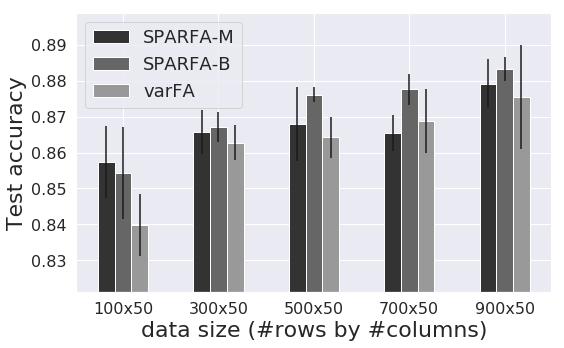
\includegraphics[width=0.4\linewidth]{sim_acc.png}
    \hspace{3pt}
    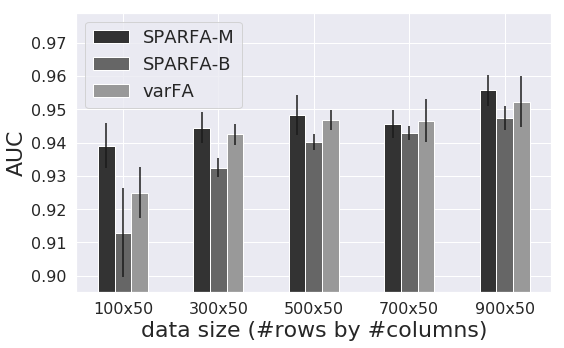
\includegraphics[width=0.4\linewidth]{sim_auc.png}
    \hspace{3pt}
    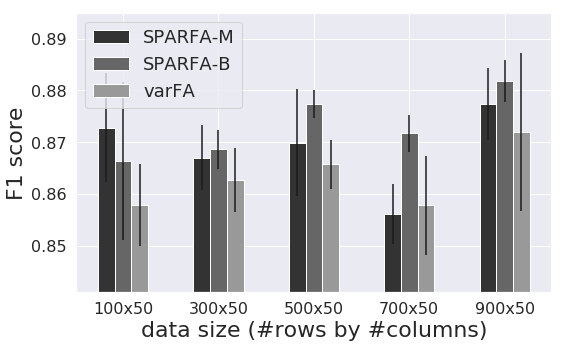
\includegraphics[width=0.4\linewidth]{sim_f1.png}
    \caption{Performance of the  SPARFA-M, SPARFA-B, and VarFA algorithms on the synthetic data set with different data sizes. Plots from left to right show comparison on accuracy (ACC), area under curve (AUC) and F1 metrics, respectively. Higher is better for all metrics. VarFA  performs
        similarly to SPARFA-M and SPARFA-B.}
    \label{fig:synthetic}
\end{figure*}

\subsection{Remarks}
%
\subsubsection*{Applicability of VarFA} The VarFA framework is general and flexible and can be applied to a wide array
of FA models. The recipe for applying VarFA to an FA model of choice is as
follows: 1) formulate the FA model into the canonical formulation as in
Eq.~\ref{eq:sparfa}; 2) partition the factors into student factor $\nu$, the
remaining unknown factors $\theta$ and known factors $\psi$; 3) perform VI on
$\nu$ and MLE estimation on $\theta$, following
Section.~\ref{sec:method-details}.

\subsubsection*{Relation to variational auto-encoders}Our proposed framework can be regarded as a standard variational auto-encoder
(VAE) but with the decoder implemented not as a neural network but by the FA
model. Because the decoder is constraint to a FA model, it is more
interpretable than a neural network.

\subsubsection*{Relation to other efficient Bayesian factor analysis methods}
We acknowledge that VI applied to general FA models have been proposed in
existing literature~\cite{ghahramani2000variational,zhao2009note}. However, to
our knowledge, little prior work have applied VI to educational FA models nor
investigated its effectiveness. One concurrent work applied VI to
IRT~\cite{wu2020variational}. Our VarFA framework applies generally to a number
of other FA models by following the recipe in the preceding paragraph,
including IRT. Thus, our work complements existing literature in providing
promising results in applying VI for FA models in the context of educational
data mining.
%
\section{Experiments}
\label{sec:experiments}
%
We demonstrate the efficacy of VarFA variational inference framework using the
sparse factor analysis model (SPARFA) as the underlying FA model.
%
This choice of SPARFA as the FA model to investigate is motivated by its
mathematical generality: it assumes no auxiliary information is available and
all three factors $\rvc_i$'s, $\rvm_j$'s and $\mu_j$'s need to be estimated,
which makes the inference problem more challenging.~\cite{lan14a} provides two
inference algorithms including SPARFA-M (based on MLE) and SPARFA-B (based on
MAP).
%
We conduct experiments on both synthetic and real data sets. Using synthetic
data sets, we compare VarFA to both SPARFA-M and SPARFA-B. We demonstrate that
1) VarFA predicts students' answers as accurately as SPARFA-M and SPARFA-B; 2)
VarFA is almost 100$\times$ faster than SPARFA-B. Using real data sets, we
compare VarFA to SPARFA-M. We demonstrate that 1) VarFA predicts students'
answers more accurately than SPARFA-M; 2) VarFA can output the same insights as
SPARFA-M, including point estimate of students' skill levels and questions'
associations with skill tags;
% \ml{you can be more specific here about what type of insights do we obtain} 
3) VarFA can additionally output meaningful uncertainty quantification for student skill levels, which SPARFA-M is incapable of, without sacrifice to computational efficiency. Note that SPARFA-B can also compute uncertainty for small data sets but fails for large data sets due to scalability issues and thus we do not compare to SPARFA-B for real data sets.
%
Specifically for SPARFA, using the notation convention in
Section~\ref{sec:FA-inference}, the question-skill association factors
$\rvm_j$'s and the question difficulty factors $\mu_j$ are collected in $\theta
    = \{\rvm_1,...,\rvm_Q,\mu_1,...,\mu_Q\}$. The student skill level factors
$\rvc_j$'s are collected in $\nu = \{\rvc_1,...,\rvc_N\}$. Because the factors
$\rvm_j$'s are unknown, the ``skills'' in SPARFA are \textit{latent} (referred
to as ``latent skills'' in subsequent discussions) and are not attached to any
specific interpretation. However, as we will see in
Section~\ref{sec:experiment-post-processing}, assuming the skill tags are
available as auxiliary information, we can associate the estimated latent
skills with the provided skills tags using the same approach proposed
in~\cite{lan14a}. For the regularization term in Eq.~\ref{eq:objective},
because the factors $\rvm_j$'s are assumed to be sparse and nonnegative, we use
$\ell1$ regularization for $\rvm_j$'s. When performing MLE for $\rvm_j$'s, we
use the proximal gradient algorithm for optimization problem with nonnegative
and sparsity requirements; see Section 3.2 in~\cite{lan14a} for more details.
For the other unknown factor $\mu_j$'s in $\theta$, we apply standard $\ell2$
regularization. The code along with instructions to reproduce our experiments
can be downloaded from~{\color{blue}{\url{https://tinyurl.com/tvm4332}}}.
%
\begin{figure}
    \tiny
    \centering
    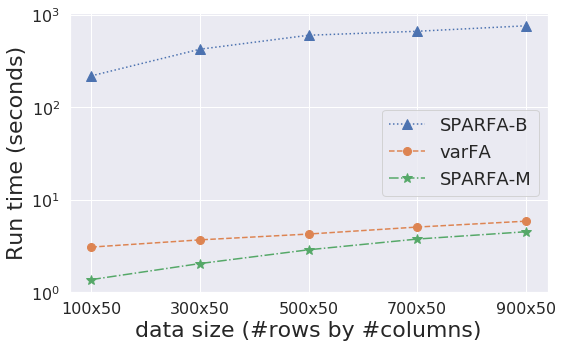
\includegraphics[width=0.4\linewidth]{sim_time.png}
    \caption{Training run time comparing VarFA, SPARFA-M, and SPARFA-B on synthetic data sets of varying sizes. VarFA performs approximate Bayesian inference almost 100x faster than SPARFA-B and is close to the run time of SPARFA-M. Thus, VarFA enables practical and scalable Bayesian inference for very large data sets.}
    \label{fig:run-time}
\end{figure}
\subsection{Synthetic Data Experiments}
\subsubsection{Setup}
%
\subsubsection*{Data set generation} We generate data set according to the canonical FA model specified in
Eq.~\ref{eq:sparfa}, taking into consideration the additional sparsity and
nonnegativity assumptions in SPARFA. Specifically, We sample the factors
$\mu_j$'s and $\rvc_i$'s from i.i.d. standard isotropic Gaussian distributions
with variance $1$ (or identity matrix for $\rvc_i$'s) and mean sampled from a
uniform distribution in range $[-1, 1]$. To simulate sparse and nonnegative
factors $\rvm_j$'s, we first sample an auxiliary variable $s_{kj}\stackrel{\rm
        i.i.d.}{\sim}{\rm Bernoulli}(\pi)$, where $\pi$ controls the sparsity, and then
sample $m_{kj}\stackrel{\rm i.i.d.}{\sim}{\rm Exponential}(1)$ when $s_{kj}=1$
or setting $m_{kj}=0$ when $s_{kj}=0$ for each $j$ and $k$. In all synthetic
data experiments, we use $\pi=0.3$ and set the true number of latent skills to
$K=5$.

%\vspace{-10pt}
\subsubsection*{Experimental settings}
We vary the size of the data set and use 5 different data matrix sizes:
100$\times$50, 300$\times$50, 500$\times$50, 700$\times$50 and 900$\times$50.
We select a data missing rate of 50\%, i.e., we randomly choose 50\% of all
entries in the data matrix as training set and the rest as test set.
Experimental results for each of the above data sizes are averaged over 5 runs
where we randomize over the train/test data split. We train SPARFA with both
SPARFA-M and VarFA using the Adam optimizer~\cite{kingma2014adam} with learning
rate $=0.05$ for 100 epochs. Regularization hyper-parameters are chosen by grid
search for each experiment. For VarFA, we use a simple 3-layer neural network
for the function $f_\phi$ in the variational distribution. We use the
hyper-parameter settings for SPARFA-B following Section 4.2 in~\cite{lan14a}.
%
\begin{table}
    \caption{Summary statistics of pre-processed real data sets.}
    %\vspace{-5pt}
    \begin{tabular}{lccc}
        \toprule
        \textbf{data set}          & \textbf{\#students} & \textbf{\#questions} & \textbf{\%observed} \\ \hline
        assistment \Tstrut \Bstrut & 392                 & 747                  & 12.93\%             \\
        algebra                    & 697                 & 782                  & 13.02\%             \\
        bridge                     & 913                 & 1242                 & 11.42\%             \\ \bottomrule
    \end{tabular}
    \label{tab:data-stat}
\end{table}

%\vspace{-10pt}
\subsubsection*{Evaluation metrics} We evaluate the inference algorithms on their ability to recover (predict) the
missing entries in the data matrix given the observed entries. We term this
criterion ``student answer prediction''. Since our data matrix is binary, using
prediction accuracy (ACC) alone does not accurately reflect the performance of
the inference algorithms under comparison. Thus, we use area under the receiver
operating characteristic curve (AUC) and F1 score in addition to ACC, as
standard in evaluating binary predictions~\cite{hastie2009elements}.
%
\subsubsection{Results}
Fig.~\ref{fig:synthetic} shows bar plots that compare the
%
student answer prediction performance of VarFA with SPARFA-M and SPARFA-B on
all three evaluation metrics. We can observe that all three methods perform
similarly and that SPARFA-M and SPARFA-B show no statistically significant
advantage over VarFA.
\sloppy
We further showcase VarFA's scalability by comparing its training run-time with SPARFA-M and SPARFA-B. The results are shown in Fig.~\ref{fig:run-time}. VarFA is significantly faster than SPARFA-B and is almost as fast as SPARFA-M.

In summary, with VarFA, we obtain posteriors that allow uncertainty
quantification with roughly the \textit{same} computation complexity of
computing point estimates and \textit{without} compromising prediction
performance.
\begin{table}[t!]
    \caption{Student answer prediction erformance comapring VarFA to SPARFA-M on Assistment, Algebra and Bridge data sets. $\uparrow$ and $\downarrow$ denote higher and lower is better, respectively. VarFA performs better than SPARFA-M on all three data sets and evaluation metrics most of the time. Additionally, VarFA's run time is very close to SPARFA-M.}
    % %\vspace{5pt}
    \centering
    \begin{subtable}{\linewidth}\centering
        \caption{Assistment}
        %\vspace{-5pt}
        \begin{tabular}{lcc}
            \toprule
            \textbf{Metric}                            & \multicolumn{2}{c}{\textbf{Algorithm}}                              \\  \hline \\[-8pt]
            % \cmidrule(l){2-2} \cmidrule(l){3-3}
                                                       & SPARFA-M                               & VarFA                      \\
            \cmidrule(l){2-2} \cmidrule(l){3-3}
            ACC $\uparrow$                             & 0.7074$\pm$0.0044                      & \textbf{0.7101}$\pm$0.0048 \\
            AUC $\uparrow$                             & 0.756$\pm$0.048                        & \textbf{0.7635}$\pm$0.0036 \\
            F1 $\uparrow$                              & 0.7746$\pm$0.0029                      & \textbf{0.7765}$\pm$0.0014 \\ \hline
            Run time (s) $\downarrow$  \Tstrut \Bstrut & \textbf{5.3319}$\pm0.2774$             & 6.9167$\pm$0.1074          \\
            \bottomrule
            %\vspace{1pt}
        \end{tabular}
        \label{tab:assistiemnt}
    \end{subtable}
    \begin{subtable}{\linewidth}\centering
        \caption{Algebra}
        %\vspace{-5pt}
        \begin{tabular}{lcc}
            \toprule
            \textbf{Metric}                           & \multicolumn{2}{c}{\textbf{Algorithm}}                              \\  \hline \\[-8pt]
            % \cmidrule(l){2-2} \cmidrule(l){3-3}
                                                      & SPARFA-M                               & VarFA                      \\
            \cmidrule(l){2-2} \cmidrule(l){3-3}
            ACC $\uparrow$                            & 0.7735$\pm$0.0037                      & \textbf{0.7774}$\pm$0.0031 \\
            AUC $\uparrow$                            & 0.8137$\pm$0.003                       & \textbf{0.8245}$\pm$0.002  \\
            F1 $\uparrow$                             & 0.8465$\pm$0.0021                      & \textbf{0.8486}$\pm$0.001  \\\hline
            Run time (s) $\downarrow$ \Tstrut \Bstrut & \textbf{8.464}$\pm$0.4568              & 10.3335$\pm$0.4435         \\
            \bottomrule
            %\vspace{1pt}
        \end{tabular}
        \label{tab:algebra}
    \end{subtable}
    \begin{subtable}{\linewidth}\centering
        \caption{Bridge}
        %\vspace{-5pt}
        \begin{tabular}{lcc}
            \toprule
            \textbf{Metric}                            & \multicolumn{2}{c}{\textbf{Algorithm}}                              \\  \hline \\[-8pt]
            % \cmidrule(l){2-2} \cmidrule(l){3-3}
                                                       & SPARFA-M                               & VarFA                      \\
            \cmidrule(l){2-2} \cmidrule(l){3-3}
            ACC $\uparrow$                             & \textbf{0.8492}$\pm$0.0016             & 0.8468$\pm$0.0016          \\
            AUC $\uparrow$                             & 0.837$\pm$0.0024                       & \textbf{0.8419}$\pm$0.0028 \\
            F1 $\uparrow$                              & \textbf{0.9121}$\pm$0.0005             & 0.912$\pm$0.0009           \\\hline
            Run time (s) $\downarrow$  \Tstrut \Bstrut & \textbf{15.6048}$\pm$0.7314            & 15.8558$\pm$1.046          \\
            \bottomrule
        \end{tabular}
        \label{tab:bridge}
    \end{subtable}
    \label{tab:real-data}
\end{table}

\begin{figure*}[t!]
    \centering
    \begin{subfigure}[b]{0.31\textwidth}
        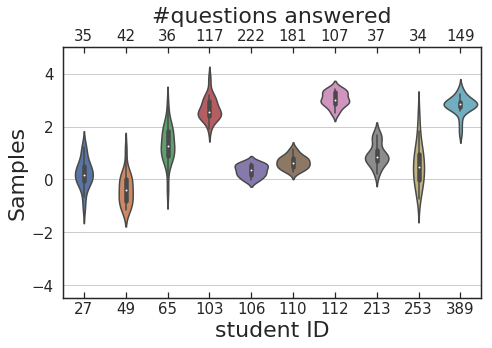
\includegraphics[width=\linewidth]{violin3.png}
        \caption{3rd latent concept}
        \label{fig:violin1}
    \end{subfigure}
    \hspace{5pt}
    \begin{subfigure}[b]{0.31\textwidth}
        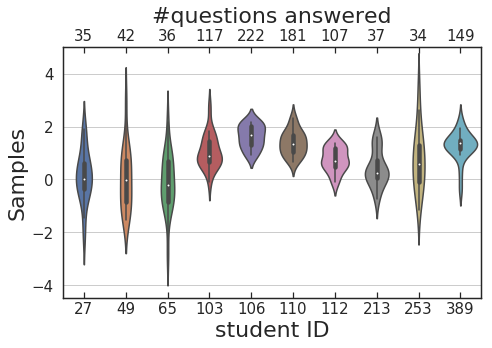
\includegraphics[width=\linewidth]{violin4.png}
        \caption{4th latent concept}
        \label{fig:violin2}
    \end{subfigure}
    \hspace{5pt}
    \begin{subfigure}[b]{0.31\textwidth}
        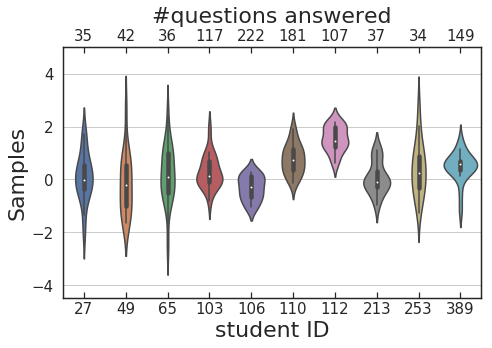
\includegraphics[width=\linewidth]{violin7.png}
        \caption{7th latent concept}
        \label{fig:violin3}
    \end{subfigure}
    \caption{Violin plot showing the mean and standard deviation of the estimated skill mastery levels on 10 selected students on the 3rd, 4th and 7th latent skills that VarFA computes. In each sub-figure, bottom and top axises respectively shows student IDs and top axis shows the number of questions each student answered. The more questions a student answers, the tighter the credible interval. (Best viewed in color.)}
    % \end{subfigure}
    \label{fig:violin}
\end{figure*}

\subsection{Real Data Experiments}
\subsubsection{Setup}
%\vspace{-10pt}
\subsubsection*{Data sets and pre-processing steps} We perform experiments on three large-scale, publicly available, real
educational data sets including ASSISTments 2009-2010 (Assistment)~\cite{assistment}, Algebra I 2006-2007 (algebra)~\cite{Algebra} and Bridge to Algebra 2006-2007 (bridge)~\cite{bridge,Stamper2016The2K}. The details of the data sets, including data format and data collection procedure can be found in the preceding references. We remove students and questions that have too few answer records from the data sets to reduce the sparsity of the data sets. Specifically, we keep students and questions that have no less than 30, 35 and 40 answer records for Assistment, Algebra and Bridge data sets, respectively.
In each data set, each student may provide more than one answer record for each question. Therefore, we also remove student-question answer records except for the first one.
Table~\ref{tab:data-stat} presents the summary statistics of the resulting pre-processed data matrix for each data set.

\subsubsection*{Experimental settings and evaluation metrics} Optimizer, learning rate, number of epochs, neural network architecture and
evaluation metrics are the same as in synthetic data experiments. For real data
sets, we use 8 latent skills instead of 5. Other choices of the number of
latent skills might result in better performance. However, since we are
comparing different inference algorithms for the \textit{same} model, it is a
fair to compare the inference algorithms on the same model with the same number
of latent dimensions.
% \ml{it's better to add an argument here justifying this choice}\jack{attempted a fix}. 
We use a 80:20 data split, i.e., we randomly sample 80\% and 20\% of the
observed entries in each data set, without replacement, as training and test
sets, respectively. Regularization hyper-parameters are selected by grid search
and are different for each data set. We only compare VarFA with SPARFA-M
because SPARFA-B does not scale to such large data sets.
%
\subsubsection{Results: Performance Comparison}
Table~\ref{tab:real-data} shows the average performance on the test set of each
data set comparing VarFA and SPARFA-M for all three data sets and additionally
run time. We can see that VarFA achieves slightly better student answer
prediction on most data sets and on most metrics.
%
Interestingly, recall that, in the preceding synthetic data set experiment,
SPARFA-M performed better than VarFA most of the time. A possible explanation
is that, for synthetic data sets, the underlying data generation process
matches the SPARFA model, whereas for real data sets, the underlying data
generation process is unknown. VarFA's better performance than SPARFA-M for
real data sets implies that VarFA is more robust to the unknown underlying data
generation process. As a result, VarFA may be more applicable than SPARFA-M in
real-world situations.

Table~\ref{tab:real-data} also shows the run time comparison between VarFA and
SPARFA-M; see the last row in each sub-table. We see that both inference
algorithms have very similar run time, showing that VarFA is applicable for
very large data sets. Notably, VarFA achieves this efficiency while also
performing Bayesian inference on the student knowledge level factor.
% 
\subsubsection{Results: Bayesian Inference With VarFA}
We now illustrate VarFA's capability of outputting credible intervals using the
Assistment data set.
%
Fig.~\ref{fig:violin} presents violin plots that show the sampled student
latent skill levels for a random subset of 10 students.
Plots~\ref{fig:violin1},~\ref{fig:violin2} and~\ref{fig:violin3} shows the
inferred students ability for the 3rd, 4th and 7th latent skill dimension. In
each plot, the bottom axis shows the student ID and the top axis shows the
total number of questions answered by the corresponding student. For each
student, the horizontal width of the violin represents the density of the
samples; the skinnier the violin, the more widespread the samples are, implying
the model's less certainty on its estimations.

\begin{table*}[t!]
    \fontsize{8pt}{8pt}\selectfont
    \caption{Illustration of the estimated latent skills with the their top 3 most strongly associated skill tags in the Assistment data set. The percentage in the parenthesis shows the association probability (summed to 1 for each latent skill). We see that the tagged skills associated with each estimated latent skill form intuitive and interpretable groups.
        % \ml{either here in the caption or in the text body, explain what these percentages mean. anything here sums to 1?}\jack{f}
    }
    \centering
    \setlength\heavyrulewidth{0.25ex}
    \begin{tabular}{p{0.45\textwidth}p{0.45\textwidth}}
        \toprule
        \textbf{Latent Skill 1}                                                                                                                                  & \textbf{Latent Skill 3}                                                                                                                                                                             \\ \hline \\[-5pt]
        \begin{tabular}[c]{@{}l@{}}Division Fractions (29.1\%)\\ Least Common Multiple (18.1\%)\\ Write Linear Equation from Ordered Pairs (17.8\%)\end{tabular} & \begin{tabular}[c]{@{}l@{}}Conversion of Fraction Decimals Percents (7.3\%)\\ Addition and Subtraction Positive Decimals (6.8\%)\\ Probability of a Single Event (5.7\%)\end{tabular} \vspace{10pt} \\ \toprule \\[-10pt]
        \textbf{Latent Skill 4}                                                                                                                                  & \textbf{Latent Skill 7}
        % \ml{- measuring CJ's ribs}}                                                                                                  
        \\ \hline \\[-5pt]
        \begin{tabular}[c]{@{}l@{}}Pattern Finding (17.4\%)\\ Histogram as Table or Graph (11.3\%)\\ Percent Of (10.5\%)\end{tabular}                            & \begin{tabular}[c]{@{}l@{}}Volume Sphere (13.4\%)\\ Volume Cylinder (10.4\%)\\  Surface Area Rectangular Prism (10.2\%)\end{tabular}                                                                \\ \bottomrule
    \end{tabular}
\end{table*}

Results in Fig.~\ref{fig:violin} confirms our intuition that the more questions
a student answers, the more certain the model is about its estimation. For
example, students with ID 106, 110 and 389 answered 222, 181 and 149 questions,
respectively, and the credible intervals of their ability estimation is quite
small. In contrast, students with ID 27, 49 and 65 answered far less questions
and the credible intervals of their ability estimation is quite large. This
result implies that VarFA outputs sensible and interpretable credible
intervals. As mentioned in Section~\ref{sec:intro}, such uncertainty
quantification may benefit a number of educational applications such as
improving adaptive testing algorithms.
%
Note that VarFA is able to compute such credible interval as fast as SPARFA-M,
making VarFA potentially useful for even real-time educational systems. In
contrast, SPARFA-M is not capable of computing credible intervals. Although we
may still obtain confidence interval as uncertainty quantification with
SPARFA-M via bootstrapping, i.e., train with SPARFA-M multiple times with
random subsets of the data set and then use the point estimates from different
random runs to compute confidence intervals. However, this method suffers from
two immediate drawbacks: 1) it is slow because we need to run the model
multiple times and 2) different runs result in permutation in the estimated
factors and thus the averaged estimations loss meaning. Given that VarFA is as
efficient as SPARFA-M and the previous drawbacks of SPARFA-M, we recommend
VarFA over bootstrapping with SPARFA-M for quantifying model's uncertainty in
practice.

\subsubsection{Results: Post-Processing for Improved Interpretability}
\label{sec:experiment-post-processing}
SPARFA assumes that each student factor $\nu_i$ identifies a multi-dimensional skill level on a number of ``latent'' skills (recall that we use 8 latent skills in our experiments). As mentioned earlier, these latent skills are not interpretable without the aid of additional information. To improve interpretability,~\cite{lan14a} proposed that, when the skill tags for each question is available in the data set, we can associate each latent skill with skill tags via a simple matrix factorization. Then, we can compute each students' mastery levels on the actual skill tags. We refer readers to Sections 5.1 and 5.2 in~\cite{lan14a} for more technical details.

Although the above method to improve interpretability has already been
proposed,~\cite{lan14a} only presented results on private data sets, whereas
here we presents results on publicly available data set with code, making our
results more transparent and reproducible.

We again use the Assistment data set for illustration. We compute the
association of skill tags in the data set with each of the latent skills and
show 4 of the latent skills with their top 3 most strongly associated skill
tags. We can see that each latent skill roughly identify the same group of
skill tags. For example, latent skill 4 clusters skill tags on statistics and
probability while latent skill 7 clusters skill tags on
geometry. Thus, by simple post-processing, we obtain an interpretation of the
latent skills by associating them with known skill tags in the data.

We can similarly obtain VarFA's estimations of the students' mastery levels on
each skill tags through the above process. In Fig.~\ref{fig:skill}, we compare
the predicted mastery level for each skill tag (only for the questions this
student answered) with the percent of correct answers for that skill tag.
Blue curve shows the empirical student's mastery level on a skill tag by
computing the percentage of correctly answered questions belonging to a
particular skill tag. Orange curve shows VarFA's estimated student mastery
level on a skill tag, normalized to range $[0,1]$.
%
We can see that, when the student gave more correct answers to questions of a
particular skill tag, such as skill tag ID 2, 10, 14 and 30, VarFA also
predicts a higher ability score for these skill tags. When the student gave
more incorrect answers to questions of a particular skill tag, such as skill
tag ID 0, 4 and 27, VarFA also predicts a lower ability score for those skill
tags. Although the correspondence is not perfect, VarFA's predicted student's
mastery levels match our intuition about student's abilities (using the
observed correct answer ratio as an empirical estimate) reasonably well. Thus,
by post-processing, we can interpret VarFA's estimated students' latent skill
mastery levels using the easily understandable skill tags.
\section{Conclusions and Future Work}
\label{sec:conclusion}
We have presented VarFA, a variational inference factor analysis framework to perform efficient Bayesian inference for learning analytics. VarFA is general and can be applied to a wide array of FA models. We have demonstrated the effectiveness of our VarFA using the sparse factor analysis (SPARFA) model as a case study. We have shown that VarFA can very efficiently output interpretable, educationally meaningful information, in particular credible intervals, much faster than classic Bayesian inference methods. Thus, VarFA has potential application in many educational data mining scenarios where efficient credible interval computation is desired, i.e., in adaptive testing and adaptive learning systems. We have also provided open-source code to reproduce our results and facilitate further research efforts.

We outline three possible future research directions and extensions. First,
VarFA currently performs Bayesian inference on the student skill mastery level
factor. We are working on extending the framework to perform full Bayesian
inference for all unknown factors. Extensions to some models such as IRT is
straightforward, as studied in~\cite{wu2020variational}, because all factors
can be reasonably assumed to be Gaussian.

However, some other models involve additional modeling assumptions, making it
challenging to design distributions that satisfy these assumptions. For
example, in SPARFA, one of the factors is assumed to be nonnegative and
sparse~\cite{lan14a}. No standard distribution fulfill these requirements. We
are exploring \textit{mixture} distributions, in particular spike and slab
models~\cite{ishwaran2005spike} for Bayesian variable selection, and methods to
combine them with variational inference,
following~\cite{titsias2011spike,enlighten191553}.

Second, other methods exist that accelerate classic Bayesian inference. Recent
works in large-scale Bayesian inference proposed \textit{approximate} MCMC
methods that scale to large data
sets~\cite{zhang2020csgmcmc,ma2015complete,song2017nice}. Some of these methods
apply variational inference to perform the
approximation~\cite{de2001variational,habib2018auxiliary}. We are investigating
extending VarFA to support approximate MCMC methods.

\begin{figure}
    \centering
    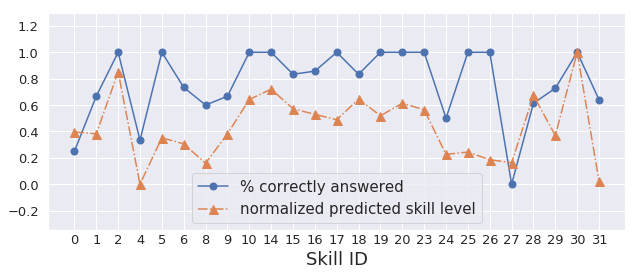
\includegraphics[width=0.8\linewidth]{student_skill.png}
    %\vspace{-15pt}
    \caption{Comparison between the estimated skill mastery levels using VarFA's predictions and using empirical observations for student with ID 110. Even though the two curves show different numeric values, they nevertheless demonstrate similar trends, showing that the predictions reasonably match our intuition about student's skill mastery levels.
        % \ml{caption too long, ugly. move some of this into the text body}
    }
    \label{fig:skill}
    %\vspace{-5pt}
\end{figure}

Finally, the goal of VarFA is to improve real-world educational systems and
ultimately improve learning. Therefore, it is necessary to evaluate VarFA
beyond synthetic and benchmark data sets. We plan to integrate VarFA into an
existing educational system and conduct a case study where students interact
with the system in real-time to understand the VarFA's educational implications
in the wild.



% The command \includeonly above allows to include a selected 
% set of chapters only.

% Uncomment the 'singlespace' environment and '\bibsep' command
% if needed - some bibliographic styles overide the definition
% of 'thebibliography' in nuthesis.cls
%
\begin{singlespace}
	%\bibsep 12pt
	\clearpage\phantomsection % needed for hyperlinks to work correctly
	\setcitestyle{numbers}
	\bibliographystyle{hunsrtnat} \nocite{*} \bibliography{citation}

\end{singlespace}

% (The following suggested by Francisco Iacobelli - 5/11/2010)
% In case, you want to use BibTeX, you should replace (or comment)
% the bibliography environment.
% Instead uncomment the following lines and replace <bib file>
% with your .bib file:
% \begin{singlespace}
% \bibsep 12pt
% \bibliographystyle{acm} %or another suitable style.
% \bibliography{<bib file>}
% \end{singlespace}

% \appendix		% Appendix begins here (optional).

% \chapter{Title of First Appendix} 	% First appendix chapter, i.e., Appendix A.

% Here goes the first appendix.

% \section{First section of Appendix}	% This is appendix section 1.

% This is the Appendix.

% \subsection{First subsection of Appendix}  % This is appendix subsection 1.

% More text ...

% \subsubsection{First subsubsection of Appendix}  % This is subsubsection 1.

% Yet more text ...

% \chapter{Title of Second Appendix}

% In case there is more than one appendix.

% \begin{vita}                    % Vita (optional).

% 	This is the Vita. This is the Vita. This is the Vita. This is the Vita. This is
% 	the Vita. This is the Vita. This is the Vita. This is the Vita. This is the
% 	Vita. This is the Vita. This is the Vita. This is the Vita. This is the Vita.
% 	This is the Vita. This is the Vita. This is the Vita.

% 	This is the Vita. This is the Vita. This is the Vita. This is the Vita. This is
% 	the Vita. This is the Vita. This is the Vita. This is the Vita. This is the
% 	Vita. This is the Vita. This is the Vita. This is the Vita. This is the Vita.
% 	This is the Vita. This is the Vita. This is the Vita.

% 	This is the Vita. This is the Vita. This is the Vita. This is the Vita. This is
% 	the Vita. This is the Vita. This is the Vita. This is the Vita. This is the
% 	Vita. This is the Vita. This is the Vita. This is the Vita. This is the Vita.
% 	This is the Vita. This is the Vita. This is the Vita.

% \end{vita}

\end{document}

